% Ce fichier main.tex est le fichier principal \`{a} partir duquel tout est g\'{e}n\'{e}r\'{e}
% This file is the main file where the final document is generated
\documentclass{these-dbl}

% Remplir les metadonnees du pdf
% Fill the pdf metadata
\hypersetup{
%    pdfauthor   = {XYZ},
%    pdftitle    = {Th\`{e}se de doctorat de XYZ},
%    pdfsubject  = {Th\`{e}se de doctorat de XYZ},
%    pdfkeywords = {mots-cl\'{e}s},
}

\geometry{vmargin=4.0cm}
\usepackage{caption}
\usepackage{subcaption}

% Spécifier vos fichiers de bibliographie
% Specify you bibliography files here
\usepackage[backend=biber, style=numeric]{biblatex}
\addbibresource{./biblio/bib.bib}

\begin{document}

% Page de garde avec commande \maketitle
% Front cover calling \maketitle
% La page de garde est en français
% The front cover is in French
\selectlanguage{french}

% Inclure les infos de chaque établissement
% Include each institution data

%%% Switch case in latex
%%% https://tex.stackexchange.com/a/343306
\makeatletter
\newcommand\addcase[3]{\expandafter\def\csname\string#1@case@#2\endcsname{#3}}
\newcommand\makeswitch[2][]{%
  \newcommand#2[1]{%
    \ifcsname\string#2@case@##1\endcsname\csname\string#2@case@##1\endcsname\else#1\fi%
  }%
}
\makeatother

%%%% Il faut adapter la taille des logos dans certains cas (e.g., EGAAL, 2 etablissements)
\newcommand\hauteurlogos[3]{
    \hauteurlogoecole{#1}
    \hauteurlogoetablissementA{#2}
    \hauteurlogoetablissementB{#3}
}

%%%%%%%%%%%%%%%%%%%%%%%%%%%%%%%%%%%%%%%%%%%%%%%%%%%
%%%%%%%%%%%%%%%% ECOLES DOCTORALES %%%%%%%%%%%%%%%%

%%%% #1: dossier des images, #2: numero ED, #3: couleur ED, #4-#5: nom complet sur plusieurs lignes
\newcommand\addecoledoctorale[5]{\direcole{#1}\numeroecole{#2}\definecolor{color-ecole}{RGB}{#3}\nomecoleA{#4}\nomecoleB{#5}}

\makeswitch[default]\ecoledoctorale{}

\addcase\ecoledoctorale{3M}{\addecoledoctorale
    {3M}
    {596}
    {193,192,183}
    {Mati\`{e}re, Mol\'{e}cules, Mat\'{e}riaux}
    {}
}
\addcase\ecoledoctorale{ALL}{\addecoledoctorale
    {ALL}
    {595}
    {240,209,134}
    {Arts, Lettres, Langues}
    {}
}
\addcase\ecoledoctorale{BS}{\addecoledoctorale
    {BS}
    {605}
    {163,219,208}
    {Biologie, Sant\'{e}}
    {}
}
\addcase\ecoledoctorale{DSP}{\addecoledoctorale
    {DSP}
    {599}
    {188,208,220}
    {Droit et Science politique}
    {}
}
\addcase\ecoledoctorale{EDGE}{\addecoledoctorale
    {EDGE}
    {597}
    {216,178,210}
    {Sciences \'{E}conomiques et sciences De Gestion}
    {}
}
\addcase\ecoledoctorale{EGAAL}{\addecoledoctorale
    {EGAAL}
    {600}
    {146,213,182}
    {\'{E}cologie, G\'{e}osciences, Agronomie et Alimentation}
    {}
    \hauteurlogos{2cm}{2cm}{2cm}
}
\addcase\ecoledoctorale{ELICC}{\addecoledoctorale
    {ELICC}
    {603}
    {249,201,188}
    {\'{E}ducation, Langages, Interactions, Cognition, Clinique}
    {}
    \hauteurlogos{2cm}{2cm}{2cm}
}
\addcase\ecoledoctorale{MathSTIC}{\addecoledoctorale
    {MathSTIC}
    {601}
    {236,115,127}
    {Math\'{e}matiques et Sciences et Technologies}
    {de l'Information et de la Communication}
}
\addcase\ecoledoctorale{SML}{\addecoledoctorale
    {SML}
    {598}
    {162,225,230}
    {Sciences de la Mer et du Littoral}
    {}
}
\addcase\ecoledoctorale{SPI}{\addecoledoctorale
    {SPI}
    {602}
    {159,182,217}
    {Sciences pour l'Ing\'{e}nieur}
    {}
}
\addcase\ecoledoctorale{STT}{\addecoledoctorale
    {STT}
    {604}
    {172,184,192}
    {Soci\'{e}t\'{e}s, temps, territoires}
    {}
}



%%%%%%%%%%%%%%%%%%%%%%%%%%%%%%%%%%%%%%%%%%%%%%%%
%%%%%%%%%%%%%%%% ETABLISSEMENTS %%%%%%%%%%%%%%%%

%%%% #1 nom du logo, #2-#4: nom complet sur plusieurs lignes
\newcommand\addetablissement[4]{\logoetablissementB{#1}\nometablissementC{#2}\nometablissementD{#3}\nometablissementE{#4}}

\makeswitch[default]\etablissement{}

\addcase\etablissement{CS}{\addetablissement
    {CS}
    {}
    {}
    {CENTRALESUP\'{E}LEC}
}
\addcase\etablissement{ECN}{\addetablissement
    {ECN}
    {}
    {}
    {L'\'{E}COLE CENTRALE DE NANTES}
}
\addcase\etablissement{EHESP}{\addetablissement
    {EHESP}
    {}
    {L'\'{E}COLE DES HAUTES \'{E}TUDES}
    {EN SANT\'{E} PUBLIQUE DE RENNES}
}
\addcase\etablissement{ENIB}{\addetablissement
    {ENIB}
    {}
    {L'\'{E}COLE NATIONALE}
    {D'ING\'{E}NIEURS DE BREST}
}
\addcase\etablissement{ENS}{\addetablissement
    {ENS}
    {}
    {L'\'{E}COLE NORMALE}
    {SUP\'{E}RIEURE RENNES}
}
\addcase\etablissement{ENSA}{\addetablissement
    {ENSA}
    {}
    {L'\'{E}COLE NORMALE SUP\'{E}RIEURE}
    {D'ARCHITECTURE DE NANTES}
}
\addcase\etablissement{ENSAB}{\addetablissement
    {ENSAB}
    {}
    {L'\'{E}COLE NORMALE SUP\'{E}RIEURE}
    {D'ARCHITECTURE DE BRETAGNE}
}
\addcase\etablissement{ENSAI}{\addetablissement
    {ENSAI}
    {}
    {L'\'{E}COLE NATIONALE DE LA STATISTIQUE}
    {ET DE L'ANALYSE DE L'INFORMATION}
}
\addcase\etablissement{ENSCR}{\addetablissement
    {ENSCR}
    {}
    {L'\'{E}COLE NATIONALE SUP\'{E}RIEURE}
    {DE CHIMIE RENNES}
}
\addcase\etablissement{ENSTA}{\addetablissement
    {ENSTA}
    {}
    {L'\'{E}COLE NATIONALE SUP\'{E}RIEURE}
    {DE TECHNIQUES AVANC\'{E}ES BRETAGNE}
}
\addcase\etablissement{IMTA}{\addetablissement
    {IMTA}
    {L'\'{E}COLE NATIONALE SUP\'{E}RIEURE}
    {MINES-T\'{E}L\'{E}COM ATLANTIQUE BRETAGNE}
    {PAYS-DE-LA-LOIRE - IMT ATLANTIQUE}
}
\addcase\etablissement{INSA}{\addetablissement
    {INSA}
    {}
    {L'INSTITUT NATIONAL DES}
    {SCIENCES APPLIQU\'{E}ES RENNES}
}
\addcase\etablissement{InstitutAgro}{\addetablissement
    {InstitutAgro}
    {L'INSTITUT NATIONAL D'ENSEIGNEMENT SUP\'{E}RIEUR}
    {POUR L'AGRICULTURE, L'ALIMENTATION ET}
    {L'ENVIRONNEMENT - ECOLE INTERNE AGROCAMPUS OUEST}
}
\addcase\etablissement{LMU}{\addetablissement
    {LMU}
    {}
    {}
    {LE MANS UNIVERSIT\'{E}}
}
\addcase\etablissement{Oniris}{\addetablissement
    {Oniris}
    {}
    {}
    {ONIRIS}
}
\addcase\etablissement{UA}{\addetablissement
    {UA-couleur}
    {}
    {}
    {L'UNIVERSIT\'{E} D'ANGERS}
}
\addcase\etablissement{UB}{\addetablissement
    {UB}
    {}
    {}
    {L'UNIVERSIT\'{E} DE BREST}
}
\addcase\etablissement{UBO}{\addetablissement
    {UBO}
    {}
    {}
    {L'UNIVERSIT\'{E} DE BRETAGNE OCCIDENTALE}
}
\addcase\etablissement{UBS}{\addetablissement
    {UBS}
    {}
    {}
    {L'UNIVERSIT\'{E} DE BRETAGNE SUD}
}
\addcase\etablissement{UN}{\addetablissement
    {UN-noir}
    {}
    {}
    {L'UNIVERSIT\'{E} DE NANTES}
}
\addcase\etablissement{UR1}{\addetablissement
    {UR1-noir}
    {}
    {}
    {L'UNIVERSIT\'{E} DE RENNES 1}
}
\addcase\etablissement{UR2}{\addetablissement
    {UR2}
    {}
    {}
    {L'UNIVERSIT\'{E} DE RENNES 2}
}


%%%% #1-#2: nom des deux logos, #3-#7: nom complet de la double affiliation sur plusieurs lignes
\newcommand\addpairetablissements[7]{
    \logoetablissementA{#1}
    \logoetablissementB{#2}
    \nometablissementA{#3}
    \nometablissementB{#4}
    \nometablissementC{#5}
    \nometablissementD{#6}
    \nometablissementE{#7}
}

% ALL, STT: UR2-ENSAB
\addcase\etablissement{UR2-ENSAB}{\addpairetablissements
    {ENSAB}
    {UR2}
    {}
    {L'\'{E}COLE NORMALE SUP\'{E}RIEURE}
    {D'ARCHITECTURE DE BRETAGNE}
    {D\'{E}LIVR\'{E}E CONJOINTEMENT AVEC}
    {L'UNIVERSIT\'{E} DE RENNES 2}
    \hauteurlogos{2cm}{1.2cm}{2cm}
}
% BS, DSP, MathSTIC: UR1-UR2
\addcase\etablissement{UR1-UR2}{\addpairetablissements
    {UR2}
    {UR1-noir}
    {}
    {}
    {L'UNIVERSIT\'{E} DE RENNES 2}
    {D\'{E}LIVR\'{E}E CONJOINTEMENT AVEC}
    {L'UNIVERSIT\'{E} DE RENNES 1}
    \hauteurlogos{2cm}{2cm}{2cm}
}
% DSP, EDGE: UR1-EHESP
\addcase\etablissement{UR1-EHESP}{\addpairetablissements
    {EHESP}
    {UR1-noir}
    {}
    {L'UNIVERSIT\'{E} DE RENNES 1}
    {D\'{E}LIVR\'{E}E CONJOINTEMENT AVEC}
    {L'\'{E}COLE DES HAUTES \'{E}TUDES}
    {EN SANT\'{E} PUBLIQUE DE RENNES}
    \hauteurlogos{2cm}{2cm}{2cm}
}
% EGAAL: UA-LMU
\addcase\etablissement{UA-LMU}{\addpairetablissements
    {LMU}
    {UA-couleur}
    {}
    {}
    {LE MANS UNIVERSIT\'{E}}
    {D\'{E}LIVR\'{E}E CONJOINTEMENT AVEC}
    {L'UNIVERSIT\'{E} D'ANGERS}
    \hauteurlogos{2cm}{1cm}{2cm}
}
% MathSTIC: UR1-InstitutAgro
\addcase\etablissement{UR1-InstitutAgro}{\addpairetablissements
    {InstitutAgro}
    {UR1-noir}
    {L'INSTITUT NATIONAL D'ENSEIGNEMENT SUP\'{E}RIEUR}
    {POUR L'AGRICULTURE, L'ALIMENTATION ET}
    {L'ENVIRONNEMENT - ECOLE INTERNE AGROCAMPUS OUEST}
    {D\'{E}LIVR\'{E}E CONJOINTEMENT AVEC}
    {L'UNIVERSIT\'{E} DE RENNES 1}
    \hauteurlogos{1.8cm}{1.3cm}{1.5cm}
}
% SML: UBO-IMTA
\addcase\etablissement{UBO-IMTA}{\addpairetablissements
    {IMTA}
    {UBO}
    {L'\'{E}COLE NATIONALE SUP\'{E}RIEURE}
    {MINES-T\'{E}L\'{E}COM ATLANTIQUE BRETAGNE}
    {PAYS-DE-LA-LOIRE - IMT ATLANTIQUE}
    {D\'{E}LIVR\'{E}E CONJOINTEMENT AVEC}
    {L'UNIVERSIT\'{E} DE BRETAGNE OCCIDENTALE}
    \hauteurlogos{2cm}{1.8cm}{1.8cm}
}
% SPI: ECN-ENSA
\addcase\etablissement{ECN-ENSA}{\addpairetablissements
    {ENSA}
    {ECN}
    {}
    {L'\'{E}COLE NORMALE SUP\'{E}RIEURE}
    {D'ARCHITECTURE DE NANTES}
    {D\'{E}LIVR\'{E}E CONJOINTEMENT AVEC}
    {L'\'{E}COLE CENTRALE DE NANTES}
    \hauteurlogos{2cm}{1.8cm}{1.8cm}
}
% SPI: UBO-ENIB
\addcase\etablissement{UBO-ENIB}{\addpairetablissements
    {ENIB}
    {UBO}
    {}
    {L'\'{E}COLE NATIONALE}
    {D'ING\'{E}NIEURS DE BREST}
    {D\'{E}LIVR\'{E}E CONJOINTEMENT AVEC}
    {L'UNIVERSIT\'{E} DE BRETAGNE OCCIDENTALE}
    \hauteurlogos{2cm}{1.8cm}{1.6cm}
}
% SPI: UN-Oniris
\addcase\etablissement{UN-Oniris}{\addpairetablissements
    {Oniris}
    {UN-noir}
    {}
    {}
    {ONIRIS}
    {D\'{E}LIVR\'{E}E CONJOINTEMENT AVEC}
    {L'UNIVERSIT\'{E} DE NANTES}
    \hauteurlogos{2cm}{2cm}{2cm}
}
% STT: ENSA-UN
\addcase\etablissement{ENSA-UN}{\addpairetablissements
    {ENSA}
    {UN-noir}
    {}
    {L'\'{E}COLE NORMALE SUP\'{E}RIEURE}
    {D'ARCHITECTURE DE NANTES}
    {D\'{E}LIVR\'{E}E CONJOINTEMENT AVEC}
    {L'UNIVERSIT\'{E} DE NANTES}
    \hauteurlogos{2cm}{2cm}{2cm}
}


% Inclure infos de l'école doctorale
% Include doctoral school data
% (3M ALL BS DSP EDGE EGAAL ELICC MathSTIC SML SPI STT)
\ecoledoctorale{MathSTIC}

% Inclure infos de l'établissement
% Include institution data
\etablissement{UBO}

%Inscrivez ici votre sp\'{e}cialit\'{e} (voir liste des sp\'{e}cialit\'{e}s sur le site de votre \'{e}cole doctorale)
%Indicate the domain (see list of domains in your ecole doctorale)
\spec{Informatique}

%Attention : le pr\'{e}nom doit être en minuscules (Jean) et le NOM en majuscules (BRITTEF) 
%Attention : the first name in small letters and the name in Capital letters 
\author{Thomas ALVES}

% Donner le titre complet de la th\`{e}se, \'{e}ventuellement le sous titre, si n\'{e}cessaire sur plusieurs lignes 
%Give the complete title of the thesis, if necessary on several lines
\title{Visualisation et Interactions avec une Colonie d'Abeilles Virtuelle}
\lesoustitre{Simulation, complexit\'{e} et pédagogie. VERSION PROVISOIRE}

%Indiquer la date et le lieu de soutenance de la th\`{e}se 
%indicates the date and the place of the defense 
\date{(Prévue) 10 Décembre 2021}
\lieu{Brest}

%Indiquer le nom du (ou des) laboratoire (s) dans le(s)quel(s) le travail de th\`{e}se a \'{e}t\'{e} effectu\'{e}, indiquer aussi si souhait\'{e} le nom de la (les) facult\'{e}(s) (UFR, \'{e}cole(s), Institut(s), Centre(s)...), son (leurs) adresse(s)... 
%Indicates the name (or names) of research laboratories where the work has been done as well as (if desired) the names of faculties (UFR, Schools, institution...
\uniterecherche{Lab-STICC CNRS UMR 6285}

%Indiquer le Numero de th\`{e}se, si cela est opportun, ou laisser vide pour faire disparaitre cet ligne de la couverture
%Indicate the number of the thesis if there is one. otherwise leave empty so the line disappeurs on the cover
%\numthese{« si pertinent »} % \numthese{}

%Indiquer le Pr\'{e}nom en minuscules et le Nom en majuscules, le titre de la personne et l’\'{e}tablissement dans lequel il effectue sa recherche  
%Indicates the first name on small letters and the Names on capital letters, the person's title and the institution where he/she belongs to.
%Exemples :  Examples :
%%%- Professeur, Universit\'{e} d’Angers 
%%%- Chercheur, CNRS, \'{e}cole Centrale de Nantes 
%%%-  Professeur d’universit\'{e} – Praticien Hospitalier, Universit\'{e} Paris V  
%%%-  Maitre de conf\'{e}rences, Oniris 
%%%- Charg\'{e} de recherche, INSERM, HDR, Universit\'{e} de Tours  
 %S’il n’y a pas de co-direction, faire disparaitre cet item de la couverture  
 %In there is no co-director, remove the item from the cover
\jury{
%{\normalTwelve \textbf{Rapporteurs avant soutenance :}}\\ \newline
%\footnotesizeTwelve
%\begin{tabular}{@{}ll}
%Yves DUTHEN & Professeur des Universités, Université Toulouse 1 Capitole, Toulouse \\
%Sébastien PICAULT & Chargé de Recherche, HDR, INRAE Oniris, Nantes\\
%\end{tabular}

\vspace{2\baselineskip}
{\normalTwelve \textbf{Composition du Jury :}}\\ \newline
%{\fontsize{9.5}{11}\selectfont {\textcolor{red}{\textit{Attention, en cas d’absence d’un des membres du Jury le jour de la soutenance, la composition du jury doit être revue pour s’assurer qu’elle est conforme et devra être répercutée sur la couverture de thèse}}}}\\ \newline
\footnotesizeTwelve
\begin{tabular}{@{}lll}

Pr\'{e}sident :        & Pr\'{e}nom NOM & Fonction et \'{e}tablissement d'exercice \textit{(à préciser après la soutenance)} \\
Rapporteurs :          & Yves DUTHEN & Professeur des Universités, Université Toulouse 1 Capitole, Toulouse \\
                       & Sébastien PICAULT & Chargé de Recherche, HDR, INRAE Oniris, Nantes\\
Examinateurs :         & Pierre CHEVAILLIER & Professeur des Universités, École Nationale d'Ingénieurs de Brest, Plouzané \\
                       & Julie DUGDALE & Maître de Conférences des Universités, HDR, Université Grenoble Alpes, Grenoble\\
                       & Huyen NGUYEN & Maître de Conférences des Universités, Université paris-Saclay, Orsay \\
Dir. de th\`{e}se :    & Vincent RODIN & Professeur des Universités, Université de Brest, Brest \\
Co-dir. de th\`{e}se : & Thierry DUVAL & Professeur Institut Mines-Télécom, IMT Atlantique, Plouzané \\
Encadrant : & Jérémy RIVIERE & Maître de Conférences des Universités, Université de Brest, Brest \\
\end{tabular}

\vspace{\baselineskip}
{\normalsize \textbf{Invit\'{e} :}}\\ \newline
\footnotesize
\begin{tabular}{@{}ll}
Frank SINGHOFF & Professeur des Universités, Université de Brest, Brest\\
 & Membre du \textit{GDSA 29}
\end{tabular}

\vspace{2.0cm}
}


\maketitle


% Sélectionner la langue du contenu suivant cette ligne
% Select the content language following this line
\selectlanguage{french}

% Inclusion du chapitre remerciement
% Input acknowledgement chapter
\clearemptydoublepage
\chapter*{Acknowledgement}

Je tiens à remercier  \\
I would like to thank. my parents..\\
J'adresse également toute ma reconnaissance à .... \\
....


% Ne pas oublier cette commande qui g\'{e}n\`{e}re la page de couverture avant
% This command will generate the front cover
\frontmatter
\clearemptydoublepage
\renewcommand{\contentsname}{Table of Contents}
\tableofcontents %sommaire %table of content
%\shorttableofcontents{Sommaire}{0}
\listoffigures

\clearemptydoublepage
\chapter*{Introduction}
\addcontentsline{toc}{chapter}{Introduction}
\chaptermark{Introduction}

Orga Abeille - Visu Interagir avec - Simuler - Modeliser - (pk existant pas bon)proposition Modele motivation (orga++) - Eval Ccl (motivation mieux) - Enfin intéragir et visu\\
\begin{itemize}
	\item Colonie d'abeille en tant que système complexe. Beaucoup de recherche sur les butineuses mais moins sur l'intérieur de la ruche.
	\item Multi agent car concentration sur les individus et leurs interactions
	\item Comprendre l'auto organisation interne par la modélisation SMA vs Équation différentielles - de l'importance des contacts individuels.	
	\item Transmettre et faciliter l'apprentissage avec l'environnement immersif.
\end{itemize}

\clearemptydoublepage
\mainmatter
\chapter{État de l'Art: Simulation Multi-Agents et Répartition des Tâches}

	Afin de comprendre et reproduire les capacités complexes des insectes sociaux, ils sont étudiés depuis une cinquantaine d'années dans le domaine des Simulations Multi-Agents (SMA). Plusieurs travaux ont ainsi pu reproduire et approcher leurs phénoménales capacités d'auto-organisation dynamique par la simulation, notamment Swarm Intelligence \cite{bonabeau_natural_1999} et bien d'autres \cite{drogoul_simulation_1993, schmickl_taskselsim_2008, dornhaus_task_1998}. Ce chapitre présente quelques modèles théoriques présents dans la littérature servant à modéliser ces systèmes, ainsi que quelques applications de ceux-ci, dans le cadre de la simulation d'insectes sociaux, et d'autres.
	
    \subsubsection*{Modèles Mathématiques}
		Bien que nous parlions ici de simulations multi-agents, il est tout de même intéressant d'en observer leurs principales alternatives, les simulations mathématiques. Souvent à base d'équations différentielles, ces modèles permettent de rendre compte d'évolution de populations par rapport à des paramètres de haut niveau. Un des premiers et des plus cités est le système d'équations "Proies-Prédateurs" de V.Volterra \cite{volterra_variations_1928}, rendant compte des fluctuations de deux populations, l'une se nourrissant de l'autre, en deux équations différentielles inter-connectées, prenant la forme :
		
		\begin{equation}
  			\left\{\begin{array}{@{}l@{}}
    			\frac{dN_1}{dt}=(\epsilon_1-\gamma_1 N_2) N_1\\
      			\frac{dN_2}{dt}=(- \epsilon_2 + \gamma_2 N_1) N_2
  			\end{array}\right.\,
		\end{equation}
		
		\begin{figure}
		\centering
		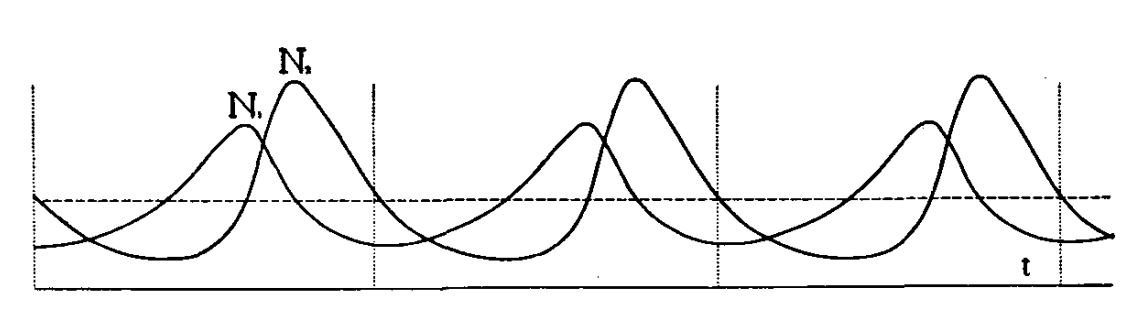
\includegraphics[width=0.9\textwidth]{./Pictures/Graphs/Volterra.JPG}
		\caption{[V.Volterra, 1928] \cite{volterra_variations_1928} Évolution des populations du système mathématique "Proies-Prédateurs", avec $N_2$ écrit en haut et $N_1$ écrit dessous.}
		\label{volterra}
		\end{figure}
		
		avec $N_1$ et $N_2$ les populations des deux espèces en nombre d'individus, respectivement les proies et les prédateurs. $\epsilon_1$ représente le taux de croissance des proies en absence de prédateur, et $\epsilon_2$ le taux de décroissance des prédateurs en l'absence de proie. Ensuite, $\gamma_1$ représente l'efficacité de chasse des prédateurs ainsi que l'efficacité de fuite des proies, là où $\gamma_2$ peut représenter l'efficacité des prédateurs à convertir les proies en descendance, ce qui revient un peu au même. $\frac{dN_1}{dt}$ représente les variations de la population des proies au cours du temps, et $\frac{dN_2}{dt}$ celles des prédateurs. la Figure \ref{volterra} nous viens de ses travaux et illustre ce système d'équations en fonction du temps, pour des paramètres choisi par l'auteur. Nous allons décrire ces équations, en prenant l'exemple très classique d'une population de loups $N_2$ confrontée à une population de moutons $N_1$. Plus les loups sont nombreux ($N2$ est grand) plus les moutons se font chasser : $\gamma_1 N_2$ est élevé, la croissance de $N1$ est alors diminuée car $\epsilon_1$ devient de plus en plus faible par rapport à $\gamma_1 N_2$. La population de moutons commence même à diminuer lorsque $\gamma_1 N_2$ devient supérieur à $\epsilon_1$, car $N1$ est alors multiplié par un nombre négatif (puisque $\epsilon_1 < \gamma_1 N_2$), la variation de population de moutons au cours du temps $\frac{dN_1}{dt}$ est alors négative, ce qui veut mathématiquement dire que la population de moutons diminue. Arrivé à un certain point, il n'y a plus assez de moutons pour la population de loups qui commence alors à s'effondrer : $-\epsilon_2 > \gamma_2 N_1$, donc $\frac{dN_2}{dt}$ est négative. Peu après, la faible population de loups transforme l'environnement en un paradis pour moutons qui voient alors leur population grimper car $\gamma_1 N_2$ étant très faible, le coefficient de $N_1$ est proche de $\epsilon_1$, la variation de population de moutons est alors proche de son maximum. Ce qui transforme peu après l'environnement en un paradis pour loups rempli de moutons, $\gamma_2 N_1$ est alors élevé, $- \epsilon_2 + \gamma_2 N_1$ et du même coup $\frac{dN_2}{dt}$ sont alors proches de leur maximum, la population de loup augmente à toute vitesse. Ensuite, tout recommence de manière cyclique, que nous retrouvons dans la Figure \ref{volterra}.
		
		Certains de ces modèles ont été créés pour simuler les évolutions de populations de colonies d'abeilles \cite{schmickl_hopomo_2007}. Bien qu'efficace, ce genre de simulation présente quelques lacunes \cite{drogoul_multi-agent_1992}. Se focalisant sur les populations, ils ne rendent pas compte des décisions prises par chaque individu, ni de leurs stratégies ou comportements. Il est de ce fait impossible pour ces simulations de prendre en compte l'importance de différents stimulus pour la réalisation de certaines actions. De la même manière, les contacts et petites interactions entre agents ne sont pas simulées. Les populations n'altèrent pas leur environnement, leurs actions sont seulement vues d'une manière probabiliste, et seuls leurs résultats sont pris en compte. De plus, les modélisations mathématiques font apparaitre des paramètres n'ayant pas vraiment de sens du point de vue du système réel, un peu à la manière des $\gamma_1$ et $\gamma_2$ de Volterra, dans son exemple pourtant très simple. Ce sont tous ces points qui nous font nous tourner vers la simulation multi-agents afin de représenter le système complexe qu'est la colonie d'abeilles, fondamentalement dépendant des interactions et contacts entre abeilles, à la plus petite des échelles.
			
			
			
	\section{Modèles existants de répartition des tâches}
	La division du travail se produit lorsque les agents doivent décider quelle tâche exécuter dans un environnement partagé. Les sociétés d'individus (ou d'agents) doivent trouver des moyens de répartir efficacement leur main-d'œuvre entre les tâches nécessaires pour survivre et s'étendre. En informatique, le contrôle décentralisé inspiré par les insectes sociaux a été étudié pendant des années et s'est avéré efficace dans de nombreuses applications. Dans cette section, nous allons passer en revue ce qui a été fait dans le domaine des modèles de répartition des tâches.
	
	
		\subsection{Foraging For Work  \cite{franks_foraging_1994}}
        Dans ce modèle, les différentes tâches que les agents doivent accomplir sont spatialement dispersées en zones. Les agents, en recherche active de travail, tentent d'exécuter la tâche associée à leur zone ou se déplacent de manière aléatoire. Ainsi, les zones surpeuplées "poussent" les agents vers les zones voisines offrant du travail, ce qui entraîne une division du travail. Lorsque de nouveaux agents apparaissent dans une zone spécifique et que les agents les plus âgés meurent à un certain âge, ce modèle assez simple recrée le polyéthisme d'âges : les agents du même âge effectuent globalement les mêmes tâches, que nous retrouvons dans les colonies d'abeilles \cite{seeley_age_1991}. En effet, la zone voyant des agents naitre va contenir plus d'agents qu'elle n'offre de travail, là ou du même temps une zone voyant des agents mourir sera dans le cas inverse. Ainsi, nous obtenons une zone de naissance qui aura tendance à repousser les agents, et la zone de "mort" va les attirer, car elle a besoin de main d'œuvre. Nous obtenons une répartition spatiale liée à l'âge des individus, nous retrouvons donc bien une forme de polyéthisme car les zones sont associées à des tâches. Ce modèle nous intéresse particulièrement pour cette capacité, en effet une des hypothèses sur la migration des nourrices vers le rôle de butineuse est qu'elle est provoquée par l'émergence de nouvelles nourrices au centre de zones de couvain, repoussant ainsi les nourrices plus âgées vers d'autres activités, ce que le \textit{Foraging For Work} est tout à fait à même de recréer.
        
        Ce modèle repose sur deux hypothèses fortes :
        
        1. Les agents doivent avoir la capacité d'évaluer les besoins de chaque tâche, leur priorité en quelque sorte. Ainsi chaque tâche est associé à un niveau de priorité, connu de l'agent.
        
        2. Les tâches sont dispersées en zones géographiques définies.
        
        
		\subsection{Modèles à Seuils}
		\label{subsectionRTM}
		\subsubsection{FTM : "Fixed Threshold Model" \cite{bonabeau_natural_1999}}
        Avec ce modèle, chaque tâche a un score, représentant sa priorité. La probabilité qu'un agent engage une tâche est directement proportionnelle à son score. Le FTM est basé sur quelques hypothèses fondatrices, dont voici la première : chaque tâche est associée à un stimulus. Le score de chaque tâche est calculé à partir de l'intensité du stimulus associé perçu par l'agent, généralement à l'aide d'une fonction sigmoïde. Soit $T$ la tâche évaluée par l'agent, $P(T)$ le score de la tâche $T$ et $S_T$ le stimulus associé (simple ou complexe) perçu par l'agent, ces fonctions prennent alors la forme :
			
\begin{equation}
\label{equationSigmoid}
	P(T) = \frac{S_T^n}{S_T^n + \Theta_T^n} \;\;\; ou \;\;\; P(T) = 1 - \frac{S_T^n}{S_T^n + \Theta_T^n}
\end{equation}	
 avec $n$ un entier pour la non-linéarité de la fonction (généralement $n=2$ \cite{schmickl_taskselsim_2008, gautrais_emergent_2002}) et $\Theta_T$ le seuil de la tâche, aussi appelé biais, de la sigmoïde. La Figure \ref{sigmoids} présente différentes sigmoïdes mettant en valeur l'impact du paramètre $\Theta_T$, propre à chaque agent. Le seuil sert en quelque sorte de point d'ancrage : lorsque le seuil est strictement équivalent au stimulus d'entrée, alors la valeur du résultat est exactement $\frac{1}{2}$. Ce biais est utilisé pour modifier la perception des agents : avec un biais très faible, les agents sont très sensibles au stimulus associé et s'engagent dans la tâche plus tôt que les agents avec un biais plus élevé \cite{dornhaus_task_1998}. 
        
        Largement utilisés pour modéliser et piloter des simulations d'insectes sociaux, les modèles à seuils reposent fortement sur l'association entre tâches et stimulus. Voici les autres hypothèses fondatrices : ils supposent également que l'exécution d'une tâche diminue le stimulus qui lui est associé, et que ne pas exécuter une tâche augmente son stimulus associé. Dans le cas contraire, les agents exécuteraient constamment cette tâche, ou du moins même jusqu'à ce qu'elle ne soit plus prioritaire. Le stimulus doit être une représentation de la priorité de la tâche qui lui est associée, à tout moment. 
        
        Par exemple, Bonabeau et al. \cite{bonabeau_quantitative_1996} utilisèrent un FTM pour modéliser la répartition du travail au sein d'une espèce de fourmi contenant deux types d'individu aux caractéristiques physiques très différentes \cite{wilson_relation_1984}. Appelés "Majors" et "Minors" dans leurs travaux, ces castes correspondent respectivement à ce que nous pourrions voir comme de grands soldats et de petites ouvrières. Dans la nature, il a été observé que les ouvrières travaillent en permanence, alors que les soldats travaillent seulement lorsque la demande est trop forte par rapport au nombre d'ouvrières présentes. Ces deux castes ont alors été modélisées, chacune avec un seuil différent pour une même tâche abstraite. Ainsi, les ouvrières ont reçu un seuil très faible, elles s'engagent donc dans la tâche même lorsque le stimulus déclencheur est relativement faible. À l'inverse, les soldats ont un seuil élevé, elles nécessitent donc un stimulus déclencheur très intense pour engager la tâche. Ainsi, lorsque le nombre d'ouvrières est suffisant pour maintenir le stimulus à un niveau faible (elles sont suffisamment nombreuse par rapport à la demande), les soldats ne travaillent pas car le stimulus n'atteindra jamais une valeur suffisamment élevée. En revanche, lorsque des ouvrières sont retirées de la simulation (ou de la colonie), le peu qui reste ne parvient plus à maintenir le stimulus bas : la demande dépasse l'offre. Le stimulus grimpe donc régulièrement, jusqu'à atteindre la seuil déclencheur pour les soldats, qui se mettent alors au travail. Ce qui est intéressant c'est que lors de la réintroduction des ouvrières, les soldats arrêterons rapidement de travailler, le stimulus déclencheur redevenant trop faible du fait du travail des nouvelles ouvrières. On obtient donc un magnifique exemple d'auto-organisation sans aucun contrôle central, sur une seule tâche et avec deux populations aux seuils fixes, mais différents.
		
		\begin{figure}
		\centering
		\includegraphics[width=0.5\textwidth]{./Pictures/Figures/sigmoids.png}
		\caption{L'influence du paramètre thêta ($\Theta$) sur la forme des sigmoides.}
		\label{sigmoids}
		\end{figure}
		
		Dans ce modèle, chaque tâche a une probabilité d'interruption aléatoire évaluée à chaque pas de temps. Par exemple, un agent peut avoir $0.5\%$ de chances d'interrompre sa tâche en cours, à chaque pas de temps \cite{gautrais_emergent_2002}. Lorsque c'est le cas, l'agent recherche une nouvelle tâche en utilisant les scores de chaque tâche. Cette interruption totalement aléatoire se repose sur les hypothèses fondatrice des modèles à seuils : le score représente directement la priorité de la tâche. Ainsi, en interrompant régulièrement l'agent, on le force à observer ces niveaux de priorité, nous assurant ainsi qu'il exécute toujours la tâche la plus prioritaire.
        
        \subsubsection{RTM : "Response Threshold Model", Renforcement du biais}
        Sur la base du FTM et de l'équation \ref{equationSigmoid}, différents travaux des années 90 \cite{theraulaz_response_1998,carbonell_multi-agent_1994, gautrais_emergent_2002} ont proposé de mettre en place des mécanismes de renforcement de la valeur $\Theta$, en modifiant la sensibilité des agents pendant l'exécution, formant ainsi efficacement des spécialistes. Cette mise à niveau du FTM est plus généralement appelée "Response Threshold Model" (RTM).
        
        Par exemple, Cicirello et Smith \cite{cicirello_wasp-like_2004} utilisèrent un modèle à seuils pour résoudre un problème d'allocation de ressource : une ligne d'assemblage de \textit{General Motors} qui doit peindre des camions tout juste assemblés, de différentes couleurs. Chaque compartiment de peinture est alors vu comme un agent qui possède une tâche par couleur de camion. Ainsi, une tâche consiste à peindre un camion d'une couleur, et changer de couleur signifie changer de tâche. Chaque tâche possède un seuil variable, permettant d'exprimer à la fois la spécialisation d'un compartiment pour une couleur, mais aussi indirectement d'exprimer le coût du changement de couleur. En effet, lors d'un changement de couleur, beaucoup de temps est perdu car il faut purger tout le système du compartiment, gâchant du même coup une bonne quantité de peinture. L'idée est donc de minimiser les coûts en peinture ainsi que le temps pour peindre une grande série de camions de couleurs différentes et inconnues \textit{a priori}. Une file de camions à peindre arrive en entrée et les compartiments doivent en accepter certains pour les peindre. Un compartiment ajuste les seuils de ses tâches à chaque pas de temps. Ainsi, il diminue celui de sa tâche correspondant à sa couleur actuelle, augmentant ses chances d'accepter de peindre un camion de cette couleur, et à l'inverse augmente les seuils de toutes ses autres tâches. Lorsqu'un compartiment n'a aucun camion à peindre, il diminue alors tous ses seuils, de plus en plus vite avec le temps qui passe.
        
        De cette manière, Cicirello et Smith arrivent à grandement limiter le nombre de changement de couleurs nécessaires, tout en conservant un rendement proche des méthodes traditionnellement utilisées pour ce genre de problème.
        
        
        \section{Applications de Modèles de Répartitions des Tâches}
        Nous nous intéressons ici à quelques applications pratiques de modèles théoriques, principalement ceux que nous venons de décrire. 
        
        \paragraph{}
        Drogoul et.al. \cite{drogoul_multi-agent_1992} ont réalisé une simulation multi-agents de colonie de fourmis, ainsi qu'un modèle de tâche et de sélection de tâches. Ils ne parlaient à l'époque (1992) pas encore de systèmes à seuils, mais en étaient déjà très proche. Dans leur modèle, chaque tâche est liée à un stimulus déclencheur, et possède un poids. Pour être sélectionnée, la tâche doit multiplier son poids et son stimulus déclencheur, et la compare à sa valeur de \textbf{seuil}. Lorsque la valeur dépasse le seuil et le niveau d'activation de la tâche courante (le produit poids - stimulus au moment de sa sélection), la tâche devient \textit{activable}. Ensuite, parmi toutes ses tâches activables, l'agent vient sélectionner celle dont le \textit{niveau d'activation} (le produit poids - stimulus) est le plus élevé (aléatoire en cas d'égalité). Une fois choisie, la tâche passe en tâche courante, et son produit poids-stimulus devient son niveau d'activation. Si aucune tâche n'est activable, le niveau d'activation de la tâche courante est réduit légèrement. Les seuils varient en fonction des activités de l'agent : ils arrivent ainsi à créer des spécialistes, des agents qui s'engagent principalement dans les même tâches. Pour ceci, à chaque sélection d'une tâche, le seuil de celle ci est légèrement abaissé, et ceux des autres tâches sont augmentés.
        
        \paragraph{}
        Nous allons désormais décrire la simulation de colonie d'abeilles de Schmickl et Crailsheim \cite{schmickl_analysing_2008}. Leur simulation se concentre principalement sur les flux de nourritures (synthétisés en nectar) au sein de la colonie. 4 Tâches sont modélisées, dont une tâche spéciale "Sans Tâche" servant de transition entre les trois autres : "Butiner", "Stocker" et "Nourrir le couvain". Chacune de ces trois tâches possède une probabilité de sélection et d'interruption. Les probabilités d'interruption sont fixes. Les probabilités de sélection proviennent d'un modèle à seuils, un score est donné par une fonction sigmoïde paramétrée par le seuil de la tâche (comme présenté plus tôt dans ce Chapitre). Un agent doit absolument interrompre sa tâche via l'interruption aléatoire, puis passer un pas de temps avec la tâche "Sans Tâche" avant de pouvoir engager une autre tâche. 
        
        Le butinage est simplifié, les butineuses sortent de la ruche et y retournent un peu plus tard, avec leur réserve de nourriture remplie. Une fois rentrée à la colonie, elles attendent une receveuse pour leur transmettre le nectar. Les butineuses vont ensuite se reposer pour un nombre de pas de temps fixes puis repartent butiner. Selon son temps d'attente $T_{search}$ en pas de temps, si $T_{search} <= 20$ la butineuse effectue une "Waggle Dance", afin de recruter plus de butineuses. Si $T_{search} >= 50$, la butineuse va effectuer une "Tremble Dance", afin de recruter plus de receveuses. Sinon l'abeille ne danse pas. Les \textit{Waggle} et \textit{Tremble Dances} sont respectivement les stimulus déclencheurs des tâches de butinage et de stockage (retrouvée dans les colonies réelles \cite{winston_biology_1991}), permettant à des abeilles sans emplois de choisir une activité. Les receveuses ayant reçu du nectar vont alors aller le stocker dans le haut de la colonie, où il sera récupéré par tous les agents ayant besoin de manger, ainsi que par les nourrices qui s'en serviront pour nourrir les larves. Ces-dernières émettent un stimulus selon leur niveau de faim, servant de stimulus déclencheur à la tâche de nourrice. Dans leurs simulations, les larves ne deviennent pas des adultes et ces-derniers ne meurent pas de vieillesse. En revanche, tous les agents peuvent mourir de faim, le point principal de cette simulation étant la distribution de nectar. Ils ont ensuite pu faire des simulations en altérant l'environnement afin d'observer la réponse de la colonie, dans son organisation. Ils ont par exemple retiré des agents d'une certaine tâche au milieu de la simulation, ou rajouté/enlevé du couvain. Ils ont pu montrer par la suite que leur système s'ajuste à ces changements, faisant apparaitre son auto-organisation. Ils concluent en disant que le stimulus déclencheur de la tâche de butinage est surement complexe, et ne peut dépendre que de stimulus externes.
        
        \paragraph{}
		Nous nous éloignons légèrement des insectes sociaux pour nous diriger vers des essaims de robots. Brutschy et. al. \cite{brutschy_self-organized_2014} proposent un modèle permettant à des robots ne communiquant pas entre eux de se répartir efficacement le travail, entre deux tâches inter connectées. En effet, la première de ces tâches est d'aller récolter une ressource. La deuxième est d'attendre qu'un robot amène une ressource dans un endroit défini, pour aller ranger cette même ressource dans la base. Nous voyons bien ici que ces tâches sont inter-dépendantes (pour utiliser leur vocabulaire) : sans robot effectuant l'une d'elle, les robots de l'autre tâche sont coincés. Afin de correctement décider quelle tâche effectuer, les robots estiment, d'après leurs perceptions, les besoins de chaque tâches. Pour ceci, une fois rendu à "l'interface" entre les deux tâches, chaque robot va maintenir une mémoire de la moyenne des temps d'attente auxquels il est confronté. Si ce temps d'attente dépasse un certain \textbf{seuil}, alors le robot va sélectionner l'autre tâche que celle qu'il effectue. Ainsi, au long de la simulation, chaque robot va affiner sa moyenne des temps d'attentes pour les deux tâches. Même s'ils ne parlent pas directement de modèles à seuils pour décrire leur proposition, il est intéressant de constater qu'ils utilisent seuils et sigmoïdes, avec toutefois une emphase sur les calculs probabilistes. Dans leur modèle, les transitions entre les tâches sont explicites : un agent ne peut sélectionner une des tâches que s'il exécute déjà l'autre. Les modèles à seuils proposent quant à eux des transitions implicites, où chaque tâche est en quelques sortes en concurrence pour être sélectionnée par l'agent. L'utilisation de perception locale afin d'estimer la pertinence de l'exécution d'une tâche par un agent est toutefois très intéressante.
        
        \paragraph{}
        Betti et.al. \cite{betti_bee_2017} proposent une simulation complexe d'une colonie d'abeilles. Avec une emphase certaine sur l'influence de l'environnement sur la vie de la colonie, notamment les pesticides et quelques parasites comme le Varroa dont nous avons parlé au Chapitre précédent, leur répartition des tâches est simplifiée. Elle est en effet dépendante des connaissances des agents ainsi que de leur âge, or tous les agents ont connaissances de la répartition courante des tâches, ainsi que des réserves de nourriture de la colonie. Les agents apparaissent en tant que larve, fécondée ou non, devenant par la suite une mâle (ne servant a rien) ou une femelle. Les ouvrières sont alors "Juvéniles" jusqu'à ce qu'elles atteignent 3 jours, elles deviennent alors nourrices. Si la colonie en a besoin, une ouvrière peut changer de rôle entre nourrice et "maintenance", qui consiste en du nettoyage. Ces ouvrières peuvent aussi devenir butineuses, elles ne reviendront alors plus en arrière. Ensuite, la simulation du butinage est assez poussée, prenant en compte l'exploration, les danses de recrutement, ainsi que l'effet des pesticides sur la précision de vol des butineuses. Il serait particulièrement intéressant de combiner leur simulation poussée du butinage et des effets des pesticides (ainsi que l'effet des autres parasites sur les larves) avec un modèle de répartition des tâches plus poussé.
        
        \paragraph{}
        Enfin, nous allons nous intéresser aux travaux Schmickl et Crailsheim \cite{schmickl_costs_2004} sur le butinage et le processus de prise de décision des agents butineurs. Afin de simuler les différentes danses effectuées par les abeilles rentrant dans la ruche, ils ont mis en place un système à seuils comprenant différentes formes de seuils, afin de s'approcher d'observations réelles de Seeley \cite{seeley_tremble_1992}. Différentes sigmoïdes sont utilisés, avec des paramètres très hétérogènes. Ces travaux nous prouvent l'efficacité des modèles à seuils à simuler des comportements différents, les faisant cohabiter de manière cohérente. Leurs abeilles peuvent alors décider de danser pour recruter d'autres butineuses, en leur communiquant la position de la source dont elles reviennent (avec de légères erreurs sur la communication). Mais elles peuvent aussi danser pour attirer et recruter des receveuses, ou même décider de ne pas danser du tout. Certaines partent après avoir suivi une danse, mais d'autres peuvent décider de partir en tant que "scout" explorer l'environnement, afin de peut être prendre connaissance d'une nouvelle source de nourriture, pour en communiquer ensuite la position avec ses collègues.
        
			
	\section*{Conclusion}
	Le modèle "Foraging For Work" nous intéresse car il permet de simuler un cas intéressant de la colonie, la migration des nourrices vers le butinage. En revanche, il ne nous permettra pas de simuler l'ensemble de la colonie. C'est pour ceci que nous nous tournons vers les modèles à seuils : les "RTM". Ils présentent trois hypothèses fondatrices pour fonctionner : chaque tâche doit être associée à un stimulus déclencheur, l'exécution de la tâche vient réduire l'intensité de son stimulus associé, qui augmente lorsque la tâche n'est pas (ou pas assez) exécutée par les agents.
	D'après nos connaissances sur les abeilles, nous trouvons des tâches qu'elles réalisent qui ne respectent pas ces deux conditions : pas de stimulus directs pour pousser au butinage (sauf quelques cas précis) ou à l'alimentation du couvain. Nous nous intéressons donc ici aux situations dans lesquelles ces hypothèses ne sont pas vraies. Aussi, si certaines tâches, notamment celles liées au couvain, peuvent être séparées en zone définie dans la ruche, ce n'est pas le cas de la majorité : le modèle FFW ne pourra donc pas nous aider à modéliser l'ensemble de la colonie.
	
	De plus, les abeilles montrent très peu de spécialisations individuelles, nous n'aurons donc pas besoin d'intégrer ce mécanisme à nos RTM \cite{kolmes_quantitative_1984}.
	
	 Nous décrivons dans le chapitre suivant notre modèle fondé sur un RTM et agrémenté d'un mécanisme supplémentaire basé sur la motivation interne pour gérer ces tâches ne respectant pas les hypothèses. Nous allons aussi devoir nous passer de l'interruption aléatoire proposée par ces modèles, qui ne fait sens que lorsque les deux hypothèses sont valides.


\clearemptydoublepage
\chapter{Proposition : Prise de Décision et Interruption}
	Dans ce chapitre et à l'aide de ce que nous venons d'apprendre au sujet de la répartition des tâches, nous allons pouvoir construire notre propre mécanisme générique, que nous utilisons ensuite pour notre cas d'application : la colonie d'abeilles (Chapitre 3). Nous allons voir comment modéliser nos tâches et comment les exécuter. Nous verrons ensuite les mécanismes de sélection, puis d'interruption que nous avons mis en place afin que nos agents effectuent toujours une tâche qui a du sens par rapport à l'état actuel de l'environnement et de l'activité des autres agents. Nous terminerons ce chapitre par un exemple possible d'application de ce modèle dans le cadre de la robotique en essaim, où une population de robot devra se partager deux tâches : collecte de ressources et patrouille.
	
	\section{Modélisation des tâches : Exécution du comportement}	
	
		\subsection{Actions, Activités et Tâches}
		\paragraph{}
			Afin de modéliser nos tâches, nous allons utiliser 3 concepts : Actions, Activités et Tâches.
			
			Une Action est définie comme une interaction avec l'environnement extérieur, non interruptible et d'une durée déterminée et courte (pas plus de quelques pas de temps, pour ne pas bloquer l'agent). Elle n'est donc pas forcément élémentaire, mais doit s'en approcher. Chaque Action possède une condition d'activation.
			
			Ensuite, une Activité est un ensemble d'Actions et/ou d'autres Activités. Une Activité possède aussi sa propre condition d'activation. Indirectement, tout ce qu'elle contient partage alors sa condition d'activation, ce qui nous permet de factoriser cette condition et d'alléger notre écriture, et ainsi de modéliser des comportements complexes.
			
			Pour finir, une Tâche est l'ensemble des Activités et Actions. On peut donc voir une Tâche comme l'Activité racine, un peu à la manière d'un système de fichiers : les Activités sont des dossiers et contiennent d'autres dossiers et/ou des fichiers, que sont les Actions.
			
		\subsection{Subsomption Hiérarchique et Exécution}
			
			\begin{figure}
			\centering
			\includegraphics[width=\textwidth]{Pictures/Figures/ModelisationTache.png}
			\caption{Modélisation d'une tâche à l'aide d'une subsomption hiérarchique.}
			\label{ModelisationTache}
			\end{figure}
		\paragraph{}
		
			Une architecture de subsomption permet de hiérarchiser différents comportements entre eux, afin d'obtenir un comportement général cohérent\cite{brooks_robust_1986}. Dans un ordre défini, la subsomption interroge tour à tour la condition d'activation de chacun de ses différents blocs comportements, et exécute le premier dont la condition est valide. Par exemple, modéliser le comportement d'un mouton peut se faire en trois blocs. Un premier bloc "Chercher à manger", toujours valide. Au dessus de celui-ci, donc avec une priorité plus importante, nous plaçons un autre bloc : "Brouter". Ce-dernier s'active lorsque le mouton a trouvé de quoi manger. Enfin, nous plaçons au sommet le bloc "Fuir", s'activant dès que le mouton perçoit un prédateur, et reste activé le temps de le semer. Ainsi, tant qu'aucun grand méchant loup n'est en vue, le mouton va brouter paisiblement. Dès qu'il en verra un, alors il pourra fuir.
			
			Afin de respecter l'aspect quasi-élémentaire des comportements, le bloc "Fuir" sera réalisé une multitude de fois. Ainsi, une seule exécution de Fuir ne fera faire au mouton qu'un pas l'éloignant du prédateur. Il va y faire appel plusieurs fois avant de considérer avoir semé le loup, tant que la condition du bloc "Fuir" sera valide.
			
			Une subsomption hiérarchique ajoute à cette structure simple, le fait que chaque bloc comportement puisse être une autre architecture de subsomption\cite{heckel_representational_2010}. Cette légère modification apporte une grande modularité dans la conception de ces architectures, et permet de modéliser des comportements plus complexes sans la lourdeur des subsomption classiques.
			
			\begin{figure}
			\centering
			\includegraphics[width=.9\textwidth]{Pictures/Figures/ExMouton.png}
			\caption{Modélisation de la tâche "Vie de Mouton" contenant tout le comportement du mouton de notre exemple.}
			\label{TacheMouton}
			\end{figure}
			
			Ce que nous avons appelé "bloc comportement" des subsomptions correspond à nos actions et activités. Les blocs qui contiennent une autre subsomption sont appelés activités, et ceux qui contiennent du comportement sont des actions. Ensuite, la subsomption en elle même est alors une tâche. La Figure \ref{ModelisationTache} présente la notion de subsomption hiérarchique contenant nos concepts définis plus tôt.
			
			Ainsi, pour qu'un agent puisse exécuter une tâche, il interroge l'activité racine puis va récursivement interroger ses composants. Chaque activité ou action interrogée va ainsi vérifier sa condition d'activation. Une activité dont l'activation est valide va alors continuer d'interroger ses composantes. On a donc une recherche en profondeur, par ordre de priorité, qui s'arrête à la première action interrogée avec une condition d'activation valide. Cette action est alors remontée à l'agent, qui pourra alors l'exécuter pendant toute sa durée. Ensuite, une fois l'action terminée, tout ce processus recommence afin de pouvoir déterminer une nouvelle action à exécuter.
			
			\paragraph{}
			Pour reprendre l'exemple du mouton, nous pouvons complexifier son comportement en transformant son Action "Fuir" en une Activité "Fuir" contenant deux Actions. L'Action prioritaire "Esquiver" a pour condition le fait de voir le loup droit devant, et consiste à fuir mais en tournant, afin d'éviter le loup. Ensuite, la deuxième action, "Pleine Puissance" est l'action par défaut, sans condition, qui consiste à courir tout droit tant que ça ne fait pas suffisamment de temps que le loup n'a pas été vu.
			
			La condition d'activation de l'activité "Fuir" définie plus tôt, le fait d'avoir vu un prédateur dans les dernières secondes/minutes, est alors nécessaire à l'activation des deux actions "Esquiver" et "Pleine Puissance" sans que nous ayons à les réécrire explicitement. La Figure \ref{TacheMouton} reprends la structure de la tâche du mouton que nous décrivons dans cette section.
			
	\section{Motivation : État de l'art}

Avant de continuer à construire notre modèle, nous avons besoin d'un mécanisme nous permettant d'améliorer les modèles à seuils dont nous avons discuté dans l'état de l'art. En effet, ceux-ci ne permettent pas de modéliser des tâches n'ayant pas de stimulus déclencheur : par exemple, la faim est un stimulus déclencheur de l'action de manger. En revanche, le stimulus déclencheur de rédiger un état de l'art, ou de ranger sa chambre, est beaucoup plus complexe. Nous proposons donc une solution simple, permettant de prendre en compte ces tâches sans stimulus tout en utilisant un modèle à seuils : en utilisant la motivation interne de l'agent. Avant d'aller plus loin dans notre utilisation de la motivation, voici un rapide état de l'art sur son utilité, et notre positionnement par rapport à celui-ci.

\paragraph{}
Pour les psychologues, la motivation est la source de l'action et guide son exécution. Deux types de motivations existent: extrinsèque (ou externe), lorsqu'une récompense est offerte par le monde extérieur, et intrinsèque (ou interne), qui n'a à voir qu'avec les croyances ou besoins de l'agent, comme l'amusement ou la curiosité. La théorie du Flow\cite{csikszentmihalyi_finding_1997}, de son côté, dit que la motivation interne d'un individu est maximale lorsque la difficulté rencontrée lors de la réalisation d'une tâche est suffisante pour susciter l'intérêt (qu'elle n'est pas ennuyeuse) mais suffisamment faible pour ne pas être décourageante (qu'elle n'est pas impossible à réaliser pour l'agent). 

On note dès lors que la motivation interne présente dans la littérature peut se diviser en deux catégories : d'un côté la motivation source, comme la faim, qui va provoquer un comportement, et de l'autre côté la motivation guide, motivation au sens d'implication, d'intérêt, qui elle sera plutôt un guide de cette action, comme la curiosité. On retrouve ces notions en éthologie, par exemple chez Lorenz\cite{lorenz_les_1984}, pour qui la motivation interne (guide), couplée à un stimulus (source), va déclencher et entretenir un comportement.
        
        
        \paragraph{}
        En intelligence artificielle, la motivation intrinsèque \textit{source} est particulièrement utilisée pour les systèmes d'apprentissage \cite{schmidhuber_formal_2010}, \textit{e.g.} pour aider ou guider des agents apprenants \cite{baldassarre_intrinsically_2013}, notamment en apportant la notion de curiosité à des agents informatiques. Certains travaux  \cite{carbonell_multi-agent_1994, maes_agent_1991} s'attachent à sa définition proche de l'éthologie, dans laquelle la motivation intrinsèque peut venir de nombreux stimulus internes différents et plus primitifs, tels que la faim ou la peur.
        
        D'autres travaux se basent sur la théorie du Flow : Un agent qui ne parvient pas à réaliser sa tâche ressent de l'anxiété et cherche une tâche moins difficile \cite{cornudella_how_2015}. De la même manière, un agent qui accomplit une tâche facile s'ennuie et passe à des tâches plus difficiles. L'idée de compétence apportée par Roohi et al.\cite{roohi_review_2018} rejoint ces notions : la compétence est, pour un agent, le sentiment d'être en contrôle et capable d'accomplir sa tâche actuelle. Ainsi, un agent ayant un niveau de compétence qu'il juge trop faible pour la tâche actuelle cherchera une tâche plus facile, plus adaptée.
        
        \paragraph{}
        Nous distinguons donc bien deux catégories dans la motivation interne. La première, que nous allons continuer à appeler la motivation source, proche de l'éthologie, décrit une motivation comme un stimulus interne servant à déclencher des comportements. Pour reprendre l'exemple de notre mouton, si voir un loup ne déclenche pas de réaction physique directe (au final ce ne sont que des pixels plus sombres sur le fond de sa rétine), son cerveau va pourtant reconnaitre le loup et faire augmenter la soudaine motivation de prendre ses jambes à son coup. On peut le voir comme si c'était la peur qui déclenchait la fuite.
        
        La deuxième, la motivation guide, proche de l'idée du \textit{Flow}, permet à l'agent de se situer par rapport à la difficulté de la tâche qu'il exécute, afin de maximiser son apprentissage, et donc d'optimiser l'usage de son temps. L'exemple de notre mouton sera ici un peu capilo-tracté, mais nous nous y tiendrons : nous souhaitons apprendre à ce mouton comment résoudre un Rubik's cube. Si le casse-tête lui est donné sans introduction, la tâche est insurmontable, décourageante. Le mouton n'apprend rien, il perd son temps et va donc naturellement se déconcentrer et essayer autre chose (peut être essayera-t-il d'apprendre à jongler avec plusieurs cubes ?). En revanche, si la courbe de difficulté est adaptée, en exercices simples et incrémentaux, le mouton apprendra bien mieux et restera concentré : la difficulté sera alors toujours adaptée à ses compétences.
        
        \paragraph{}
        Avec ces deux notions en tête, motivation source et motivation guide, nous pouvons passer à la suite de la description de notre modèle, dont la sélection et l'interruption des tâches se feront grâce à ces motivations.
			
	\section{Sélection : Modèle à Seuil}
		Maintenant que nous avons modélisé le fonctionnement interne de nos tâches, nous allons pouvoir construire le mécanisme permettant à nos agents de sélectionner la plus prioritaire.
		
			Pour cette sélection nous allons utiliser un modèle à seuil, que nous allons légèrement adapter en lui ajoutant un mécanisme d'interruption, décrit dans la section \ref{sectionInterruption}. Dans un modèle a seuil, chaque tâche possède une fonction lui permettant de calculer son score. Un agent peut ainsi sélectionner la tâche qui possède le plus élevé. Très souvent lié à un stimulus déclencheur, le score de la tâche est calculé à l'aide d'une fonction sigmoïde, paramétrée par un seuil, qui prend en entrée le stimulus (ou une combinaison linéaire de plusieurs stimulus), et nous donne en résultat le score de la tâche, comme nous avons pu le constater dans l'état de l'art, sous-section \ref{subsectionRTM}.
			
			Même si plusieurs agents sont en mesure d'effectuer la même tâche, les seuils de ses tâches lui sont propres. Chaque agent possède une instance différente des tâches, et chaque instance de tâche possède son propre seuil. En modélisant nos tâches, il arrive que certaines n'aient pas de stimulus déclencheur. C'est le cas pour les abeilles butineuses : le butinage de nectar semble être leur comportement par défaut, aucun stimulus global n'a encore été identifié. Dans ce cas, nous appliquons la notion de motivation interne \textit{source}, que nous avons décrit juste avant, pour créer un stimulus artificiel, qui sera inséré dans la sigmoïde afin de calculer le score de la tâche. Ainsi, toutes nos tâches, stimulus artificiel ou non, sont capables de produire un score cohérent. Nous pouvons alors dire d'une Tâche qu'elle est "motivée" lorsqu'elle utilise un stimulus déclencheur artificiel.
			
			Nous avons désormais à notre disposition deux mécanismes influant sur le score d'une tâche : nous pouvons jouer sur sa motivation source, et modifier son seuil. Afin de garder une approche cohérente, nous proposons de modifier le seuil pour représenter l'état interne de l'agent (caractéristiques physiques, physiologiques, etc.). De la même manière, modifier la motivation source permet de représenter un changement de perception, ou une décision de la part d'un agent.
			
			\paragraph{}
			Afin de toujours réaliser une tâche utile à la communauté, nos agents doivent très régulièrement interroger leurs perceptions, afin de se "mettre à jour". C'est pour ceci que nous avons introduis la notion d'évaluation systématique : un agent réévalue l'ensemble de ses tâches à chaque fois qu'il termine une action. C'est également pour cette raison que les actions doivent avoir une durée courte, de préférence atomique, pour permettre la mise à jour. Ce rafraichissement des perceptions est essentiel pour que le système puisse réagir face à une urgence. Même si notre mouton est paisiblement en train de brouter, il est intuitif de l'autoriser à fuir à la vue d'un loup avant d'avoir parfaitement terminé de brouter. Il doit aussi pouvoir faire une pause lors de la résolution d'un casse tête afin de se nourrir, pour ne pas mourir de faim.
		
	\section{Interruption : Motivation et Flow}
	\label{sectionInterruption}
		\subsection{Action Démotivante et Tâche Motivée}
		
			La réévaluation systématique nous autorise à ne pas avoir de mécanisme d'interruption : dans le cas général, la fluctuation des stimulus internes et externes suffit à l'agent pour effectuer la bonne tâche. En revanche, la question se pose lorsqu'une tâche possède un stimulus déclencheur artificiel, lié à une motivation source, fixe. Pour décider quand arrêter une telle tâche, nous avons besoin de ce mécanisme d'interruption. Dans ce cas, nos agents vont essayer d'estimer leur apport à la communauté dans leur tâche actuelle. Ainsi, lorsqu'un agent verra qu'il n'arrive pas à réaliser sa tâche, il sera dans l'état de malaise décrit pas le \textit{Flow} et cherchera de plus en plus à changer de tâche. Nous cherchons alors à mesurer l'efficacité de chaque agent dans sa tâche, afin de pouvoir détecter lorsqu'il arrive à la réaliser, mais surtout lorsqu'il n'y arrive pas. Il suffit alors de déterminer, dans le contenu de la tâche, quelles sont les Actions effectuées représentatives de son échec. Par exemple, un robot ayant pour tâche de récolter des ressources aura dans cet algorithme une séquence de déplacement aléatoire lorsqu'aucune ressource n'est en vue. Répéter en boucle ce déplacement aléatoire, cette Action, est un signe que ce robot n'arrive pas a correctement réaliser sa tâche, il devrait donc essayer de faire autre chose.
			
			Nous proposons alors d'ajouter aux Actions définies plus tôt le fait de pouvoir être "Démotivantes" (notées \textbf{M-} dans nos schémas). Lors de l'exécution d'une Action "Démotivante", un agent va baisser sa motivation interne d'un montant défini. Le but est d'augmenter les chances qu'il abandonne cette tâche au profit d'une autre, lors du processus de sélection. L'Action de déplacement aléatoire du robot que nous venons de citer est un bon exemple d'Action démotivante. Une action démotivante doit forcément être dans une tâche motivée : si la motivation interne ne joue aucun rôle dans la sélection de la tâche, il n'y a aucun intérêt à la diminuer.
			
			\paragraph{}
			Le fait de placer une motivation source artificielle brise une des hypothèses de base des modèles à seuil : exécuter une tâche doit faire baisser son stimulus déclencheur. Or ici, ce stimulus déclencheur étant fixe, il n'est pas du tout corrélé à la quantité de fois que son action liée est réalisée. Afin d'intégrer ces motivations au modèle à seuils que nous avons présenté plus tôt, nous modifions légèrement le calcul des scores des tâches motivées : le score d'une tâche motivée est remplacée par la motivation interne de l'agent, si c'est cette tâche que l'agent exécutait au pas de temps précédent. Ainsi, une tâche motivée est bien sélectionnée grâce à son score classique, mais est interrompue par une valeur de motivation plus basse, qui aura tendance à favoriser d'autres tâches. Lorsqu'une nouvelle tâche motivée est sélectionnée (et qu'elle n'était pas la tâche sélectionnée au pas de temps précédent), la motivation interne de l'agent est remontée à sa valeur maximale.
	
	\section{Définir un Agent}
	
	\begin{figure}
	\centering
	\includegraphics[width=\textwidth]{Pictures/Figures/ModelisationExecution.png}
	\caption[Sélection et exécution des tâches par chaque Agent, à chaque pas de temps.]{Sélection et exécution des tâches par chaque Agent, à chaque pas de temps. Si l'action en cours est terminée, l'agent va sélectionner une nouvelle tâche, en extraire l'action à réaliser puis l'exécuter.}
	\label{agentExec}
	\end{figure}		
	
		\paragraph{}
		À l'aide de ces définitions nous pouvons désormais décrire nos agents. Un agent est situé dans l'environnement, possède une série de senseurs internes et externes (comme la faim et l'odorat), et contient aussi une liste de tâches qu'il sera peut-être amené à réaliser au court de sa vie. Lors d'une sélection de tâche, l'agent pourra confronter ses perceptions courantes aux différents seuils et conditions de l'algorithme de sélection de tâche, donnés par son état interne ainsi que son environnement direct, afin de savoir quelles actions effectuer. La Figure \ref{agentExec} reprend ces notions et décrit le comportement et la prise de décision d'un agent à chaque pas de temps: si l'agent n'a pas d'Action en cours, il sélectionne une nouvelle Tâche en fonction de son état interne, de sa motivation interne et de ses perceptions, récupère l'Action à réaliser de sa Tâche nouvellement sélectionnée grâce à son architecture de subsomption hiérarchique, puis l'exécute.
		
		Parmi les perceptions internes de l'agent, nous trouvons une variable de motivation interne, servant aussi à la sélection de tâche. Associer une valeur de motivation à chaque tâche aurait aussi été possible et nous pouvons en trouver des équivalences dans d'autres travaux \cite{agassounon_scalable_2001}, nous avons donc décidé de tenter l'expérience avec une valeur transversale à toutes les tâches, liée à l'agent lui même.
		
		\paragraph{}
		Un agent peut aussi présenter des variations individuelles, un léger \textit{offset} que nous pouvons utiliser pour ajuster légèrement les seuils de ses différentes tâches, en plus des conditions internes et externes, afin de créer une population d'agents plus ou moins homogène. Via ses tâches, un agent possède des seuils variables qui lui sont propres : deux agents avec les mêmes tâches présentent le plus souvent des seuils différents.
		
	\section{Application possible à la Robotique en Essaim}
	
		\paragraph{}
			Les systèmes multi-agents sont souvents utilisés dans la mise en place d'essaims de robots, ce qu'on appelle le domaine des "Swarm Robotics". Ces essaims consistent en une grande quantité (dizaines, voire centaines) de robots simples, amenés à exécuter des tâches complexes en collectivité. L'image de la capacité de fourragement des fourmis est souvent utilisée comme cas d'application, nous avons donc construit notre exemple dans ce contexte. Un ensemble de robots va devoir ramener des ressources à leur base commune. Les ressources sont éparpillées dans l'environnement et doivent être traitées par un robot avant d'être déplacées jusqu'à la base. En plus de cette activité de collecte, les robots vont devoir assurer une surveillance de la base, en patrouillant autour. Ces robots possèdent une mémoire limitée : ils connaissent leur position ainsi que celle de la base, et peuvent se rappeler de la position de gisements de minerai qu'ils ont directement observés.
			
		De plus, nous ajoutons la notion d'outil : un robot devra posséder le bon outil pour exécuter une tâche, par exemple une pioche pour collecter des ressources, et des jumelles pour patrouiller. Les ressources brutes devront être traitées sur place avant de pouvoir être collectées puis amenées à la base.

		\paragraph{}
		Nous pouvons dès lors commencer à construire nos tâches :
		\begin{itemize}
			\item \textbf{Patrouiller} : le robot effectue des cercles larges autour de la base, observant les alentours. Il se démotive légèrement au fil du temps (noté M- sur la Figure \ref{swarmPatrol}), et un peu plus lorsqu'il croise un autre robot (noté M-- sur la Figure \ref{swarmPatrol}). Ceci permet aux robots d'éviter de patrouiller si un grand nombre de robots le fait déjà. Le seuil est élevé, sauf si l'agent est équipé des jumelles.
			\item \textbf{Collecter} : le robot parcours l'environnement aléatoirement à la recherche d'un gisement. Une fois trouvé, il traite le gisement pour collecter des ressources, puis les ramène à la base. Il se démotive légèrement à chaque pas de temps où il exécute un déplacement aléatoire. Le seuil est élevé, sauf si l'agent est équipé d'une pioche.
			\item \textbf{Recharger} : le robot se connecte à la base pour recharger ses batteries.
			\item \textbf{Mémoriser} : lorsque le robot voit un gisement qu'il ne connait pas, il l'ajoute à sa mémoire. A l'inverse, lorsqu'il ne voit pas de gisement (ou qu'il voit un gisement épuisé) là où il en avait retenu un, il l'oublie. Ainsi, un robot qui patrouille peut découvrir de nouveaux gisements, tout autant qu'un robot qui en cherche activement un.
		\end{itemize}
	
	\begin{figure}
	\centering
	\includegraphics[width=\textwidth]{Pictures/Figures/SwarmPatrol.png}
	\caption{Robotique en essaim : modélisation de la tâche de patrouille.}
	\label{swarmPatrol}
	\end{figure}
	
	\begin{figure}	
	\centering
	\includegraphics[width=\textwidth]{Pictures/Figures/SwarmForaging.png}
	\caption{Robotique en essaim : Modélisation de la tâche de collecte de ressources.}
	\label{swarmForaging}
	\end{figure}
		
		Pour \textit{Patrouiller} et \textit{Collecter}, si l'agent active la tâche sans posséder le bon outil, la tâche commencera par le faire retourner à la base pour équiper le bon. Cet outil va alors changer les seuils de ces deux tâches, priorisant celle dont l'outil est le bon. Ainsi, un agent ne changera d'outil que lorsque cela sera nécessaire, les seuils ajoutent ici une notion de coût du changement d'outil. Ensuite, si nous le souhaitons, en ajustant les valeurs des seuils bas (prioritaires) et haut (changement d'outil nécessaire) et/ou la force répulsive des actions démotivantes, nous pouvons ajuster ce coût empiriquement. Les Figures \ref{swarmPatrol} et \ref{swarmForaging} présentent respectivement nos modélisations en subsomption hiérarchique des tâches de patrouille et de collecte de ressources.
		
		Ensuite, si \textit{Recharger} a un stimulus déclencheur évident, le niveau courant de batterie, ce n'est pas le cas pour Patrouiller et Collecter. Nous leur appliquons donc une motivation source. Nous pouvons ensuite modifier ces motivations sources avec des perceptions de l'agent, sans qu'elles soient la majorité du stimulus déclencheur : nous pouvons réduire légèrement cette stimulation pour la tâche \textit{Patrouiller} lorsqu'un robot avec des jumelles est dans le champs de vision. De même, nous pouvons réduire la stimulation de \textit{Collecter} lorsqu'un robot avec une pioche est en vue, et l'augmenter lorsqu'un gisement de minerai est en vue.
			
			
				
	\section*{Conclusion}
		\paragraph{}
		Dans ce chapitre nous avons décrit notre modélisation des tâches en Activités et Actions, ainsi que l'adaptation du modèle à seuils pour notre sélection de tâches. La sélection de tâche se fait via un système à seuil adapté afin de prendre en compte les motivations source (nous venant plutôt de l'éthologie) et interne (ou guide, nous venant de la théorie du \textit{Flow}), afin d'inclure des tâches ne présentant pas de stimulus déclencheurs définis. Un score est calculé par tâche selon les perceptions et l'état interne de l'agent, et ce dernier sélectionne la tâche qui possède le plus grand score. Lorsque la tâche précédemment réalisée est une tâche motivée, le score est remplacé par la motivation guide, interne à l'agent et transversale à toutes les tâches de cet agent. Une fois la tâche sélectionnée, l'agent utilise notre architecture de tâches en subsomption hiérarchique afin d'obtenir le comportement, l'Action qu'il doit réaliser. Nous avons vu ensemble un exemple possible d'application à un essaim de robot, et nous allons désormais pouvoir aborder l'implémentation de l'application principale de ces travaux, la colonie d'abeilles.


\clearemptydoublepage
\chapter{Modélisation et Implémentation pour la Colonie d'Abeilles}

	Nous allons désormais voir ensemble l'implémentation du modèle que nous venons de décrire, appliqué au cas qui nous intéresse ici : la colonie d'abeilles. Pour une première itération, nos abeilles auront pour objectif de correctement se répartir le travail entre deux tâches principales : Nourrir le couvain et Butiner. Nous allons commencer par discuter de notre simulateur et de son architecture logicielle, puis du modèle physiologique de l'abeille adulte et du couvain, tiré de la biologie mais fortement simplifié. Nous verrons ensuite comment nous avons intégré le modèle de répartition des tâches décrit dans le chapitre précédent. Nous finirons par discuter de la calibration de ce système complexe, au plus proche de la biologie, tout en prenant en compte les différentes hypothèses et simplifications de notre modèle.
	
	\section{Description du Simulateur}
		\subsection{Architecture Logicielle}
			Pour réaliser ce simulateur, nous avions en tête quelques points clés. Cette thèse s'inscrit dans un projet plus grand, l'idée était donc de produire un simulateur propre, qui serai simple d'entretien et facile à améliorer et complexifier par la suite. De plus, notre bonne maitrise du langage Java, ainsi qu'un compromis entre confort d'écriture et performances nous a poussé à utiliser ce langage. Pour nous aider à mettre en place ces notions de propreté du code, nous avons utilisé des Interfaces Java, permettant de découpler des grande parties du programme, facilitant l'implémentation de modifications. Nous avons, le plus possible, pensé l'architecture en composants indépendants échangeant le moins d'informations possibles. Nous allons désormais décrire les principaux composants de cette architecture, la Figure \ref{ArchiLogicielle} résume le tout graphiquement.
			
			Le simulateur, en bon projet orienté objet, est pensé en couches d'abstraction successives. Au plus haut niveau, nous trouvons le lanceur, la classe \textit{BeekeeperLauncher}, le célèbre "\textit{main}", qui se charge des simulations. Il Présente deux modes :
	\begin{itemize}
		\item Interactions : mode pour lequel le simulateur est construit. Ce mode permet de lancer une simulation et prends en compte les interactions de l'utilisateur (via le réseau) pour altérer le comportement de la simulation.
		\item Barrage de Simulations : mode permettant de lancer un grand nombre de simulation à la suite, sans interactions possibles. Ce mode sert principalement pour calibrer certains paramètres.
	\end{itemize}				
			
			 Dans le mode "Interactions", le lanceur prépare le composant réseau qui servira à envoyer et recevoir les informations de l'application interactive, composant qui n'est pas instancié dans le mode "Barrage de Simulations". Le lanceur instancie ensuite le \textit{MainController}, le contrôleur principal, et lui partage le composant réseau si besoin. Le \textit{MainController} se charge de gérer une simulation. Désormais nous trouvons deux comportements différents pour les modes : en "Barrage de Simulations", les simulations s'enchainent à pleine vitesse, souvent en variant quelques paramètres. En mode "Interactions", lorsque la simulation est arrêtée, soit le programme s'arrête soit une autre est relancée avec les mêmes paramètres, selon ce qui a été décidé par l'utilisateur.
			 
			\begin{figure}
			\centering
			\includegraphics[width=\textwidth]{./Pictures/Figures/ArchiStart.png}
			\caption{Sequencement de l'initialisation d'une simulation.}{1- Le lanceur \textit{BeekeeperLauncher} instancie et initialise le \textit{MainController} qui se chargera d'une simulation. 1b- Dans le cas où le lanceur est dans le mode Interactions, il instancie un \textit{NetworkManager} et en donne la référence au MainController (Lors d'un changement de simulation, le \textit{MainController} est remplacé mais le \textit{NetworkManager} reste le même). 2- Le \textit{MainController} se charge désormais d'instancier un \textit{CombManager} avec les bons paramètres. 3- Le \textit{CombManager} commence par initialiser les \textit{Cadres}, il instancie en réalité des faces de cadres qu'il va associer par deux pour former les cadres de la simulation. 4- Une fois créés, les \textit{Cadres} sont alors peuplés par le \textit{CombManager} avec des \textit{Agents}. 5- Ensuite, des \textit{StimuliManager} sont instanciés par le \textit{CombManager} et associés à des faces de cadres.}
			\label{ArchiStart}
			\end{figure}
			
			\begin{figure}
			\centering
			\includegraphics[width=\textwidth]{./Pictures/Figures/ArchiLogicielle.png}
			\caption{Diagramme de classe esquissant l'architecture logicielle du simulateur.}
			\label{ArchiLogicielle}
			\end{figure}
			
			Le \textit{MainController} gère une simulation, une colonie d'abeilles. Il se charge d'instancier correctement les différents composants d'une simulation, et du bon déroulement de l'ensemble. Il compte les pas de temps, ce qui lui permet d'envoyer un signal aux agents, via un autre composant, leur ordonnant de vivre un pas de temps, ou lorsqu'il est temps de "logger". Via une interface Java, il offre un grand nombre de services haut niveau à différents composants, notamment au \textit{CombManager}, le manager des cadres, qu'il instancie avec les bons paramètres. Le \textit{CombManager} se charge d'instancier le bon nombre de faces de cadres, qui seront associées par deux en deux pour former les cadres, puis instancie les agents initiaux et les répartis sur ces cadres, via un autre composant, l'\textit{AgentFactory}, qui simplifie et centralise la création d'agents. La Figure \ref{ArchiStart} illustre les différentes interactions entre composants logiciels lors de l'initialisation d'une simulation.
			
			Chaque face de cadre possède une liste de cellules, des \textit{Cell}, qui elles même possèdent quelques attributs : leur numéro et leur position x et y sur le cadre ($numéro = y * largeur + x$), ainsi qu'une place "visite" pour un agent qui serait au dessus de la cellule, et une place "contenu", pour un agent à l'intérieur de la cellule ou de la nourriture, ou même rien, pour une cellule vide. Chaque face de cadre possède une liste contenant tous les agents que contiennent ces cellules. Cette liste agit comme un raccourcis, et permet de ne pas avoir à interroger toutes les cellules à chaque fois qu'on veut accéder aux agents. Le \textit{CombManager} possède aussi une liste d'agents, ceux qui n'appartiennent à aucun cadre, la liste de tous les agents à l'extérieur de la ruche, les butineuses.
			
			Le \textit{CombManager} est aussi responsable de la création, mise à jour, et bonne association des \textit{StimuliManager}, les managers de propagation des différents stimulus dans l'environnement. Chaque cadre a deux faces, et sont placés côte à côte. Ainsi, les faces se faisant face partagent le même \textit{StimuliManager}. 
			
			%POUR LES INTERACTIONS AVEC LE MODELE
			%Lorsque les cadres sont déplacés, de nouveaux \textit{StimuliManager} temporaires doivent être créés pendant le déplacement, puis lorsqu'ils sont reposés dans la ruche, le \textit{CombManager} se charge de refaire les bonnes associations, et combinaisons avec les temporaires.
			
			Un \textit{StimuliManager} est une grille 2D de la même taille qu'un cadre, dont chaque case possède plusieurs flottants, représentant les intensités des différents stimulus présents sur le cadre. Sa mise à jour utilise une méthode de "\textit{double buffering}" : la grille est lue et une deuxième est remplie avec les nouvelles valeurs. Une fois la lecture terminée, la deuxième grille prend la place de la première. La propagation se fait à chaque pas de temps pour chaque stimulus, afin de gagner du temps, l'évaporation se fait en même temps que le calcul de la propagation. Pour propager les stimulus, nous utilisons une fonction proche d'un flou en traitement d'image. Chaque pixel devient une moyenne pondérée de lui même et de tous ses voisins. Pour nous, chaque cellule voit sont intensité devenir la moyenne pondérée de sa propre intensité et de celles de ses voisines, en suivant cette équation :
			
			\begin{figure}
			\centering
			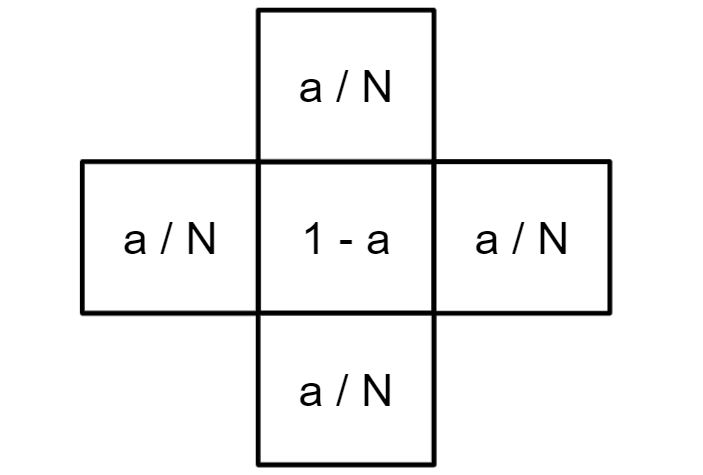
\includegraphics[width=0.4\textwidth]{./Pictures/Figures/flou.JPG}
			\caption{Filtre utilisé pour connaitre la nouvelle valeur de l'intensité du stimulus évalué. Avec $a$ la volatilité du stimulus évalué, et $N$ le nombre de voisin, ici $N=4$. Chaque pixel prend alors comme valeur la combinaison linéaire de sa valeur et de celles de ses voisins avec ce filtre pour coefficient.}
			\label{flou}
			\end{figure}
			
			\begin{equation}
			V0_{t+1} = p * ((1-a) * V0_t + \sum_{n=1}^{N} Vn_t * \frac{a}{N})
			\end{equation}
			
			Avec $V0_t$ la cellule évaluée à l'instant $t$, $Vn$ ses voisines et $N$ le nombre total de voisines. Nous utilisons aussi $a$ et $p$ deux paramètres de stimulus: la propagation dans l'espace $a$ (volatilité) et dans le temps $p$ (évaporation/amortissement). Ces paramètres nous permettent d'obtenir des comportements variés partageant les mêmes mécanismes. La figure \ref{flou} illustre cette équation sous la forme d'un filtre. Les valeurs d'évaporations sont alors utilisées sous la forme "par pas de temps". Pour mieux les contrôler, nous utilisons l'équation suivante pour les exprimer en demie-vie (durée après laquelle le stimulus aura perdu la moitié de son intensité), notion plus courante en biologie, puis les convertir en valeurs "par pas de temps" utilisables par l'algorithme :
			
			\begin{equation}
			k = \exp(\frac{-ln(2) * C}{\lambda})
			\end{equation}
			
			Avec $\lambda$ la demie vie en seconde, $C$ le coefficient appliqué pour convertir des secondes en pas de temps, et $k$ le coefficient à appliquer à chaque pas de temps pour obtenir une demie-vie de $\lambda$.
			
			\subsection{Architecture des Agents}
			Avec les mêmes objectifs en tête, lisibilité et facilité d'ajouts, nos agents ont été pensés en niveaux d'abstraction successifs. Au plus haut niveau nous trouvons la classe abstraite \textit{Agent}, qui regroupe l'âge, la position, l'énergie, la faim, une fonction abstraite \textit{live()}, ainsi que des fonctions de déplacement simples, comme le mouvement aléatoire. Nous définissons ensuite la classe \textit{EmitterAgent}, ou Agent Émetteur, qui hérite d'\textit{Agent} et ajoute les interactions avec un \textit{StimuliManager}, permettant d'émettre, ressentir des stimulus dans l'environnement. Enfin, héritant d'\textit{EmitterAgent}, nous trouvons la classe \textit{WorkingAgent}, ou Agent Travailleur, qui implémente enfin \textit{live()}, avec l'algorithme de sélection de tâches. La figure \ref{ArchiLogicielle} reprends aussi cette architecture. La fonction \textit{live()} se déroule en quelques étapes. D'abord on vérifie si l'agent est toujours en vie, ensuite nous mettons à jours ses perceptions. L'algorithme de sélection et exécution des tâches est alors appliqué, puis une fonction abstraite est appelée, fonction permettant de faire avancer le métabolisme de l'agent, et qui est implémentée différemment par nos différentes implémentations de \textit{WorkingAgent}. Nous avons pour l'instant 3 classes implémentant \textit{WorkingAgent}, les classes d'abeille adulte \textit{AdultBee}, de couvain \textit{BroodBee}, et de reine \textit{QueenBee}. Chacune de ces implémentations ajoute différentes tâches à sa liste de tâches (que nous allons décrire Section \ref{sectionModelColonie}), et implémente la fonction d'avancée du métabolisme.
			
			Ainsi, dans les plus hautes couches d'abstraction, les différents composants ont des références \textit{Agent}, ce qui améliore la modularité du programme, facilitant l'ajout de nouvelles implémentations de \textit{WorkingAgent} à l'avenir. 
			
			\subsection{Pas de temps et Multi-Thread}
			Afin d'accélérer nos simulations pour d'itérer plus confortablement dessus, nous avons mis en place un système de parallélisation, aussi appelé \textit{multi-thread}. Chaque duo de faces de cadres se faisant face, ainsi que le groupe des butineuses, vivent en concurrence, car ces différents ensembles n'interagissent pas entre eux. Pour ceci nous avons créé une classe \textit{WorkDispatcher}, qui s'occupe de gérer un groupe de \textit{thread}, de leur répartir le travail, d'en créer de nouveaux si nécessaire et de surveiller le moment où tous ont terminé leur travail. À chaque pas de temps, sur signal du \textit{MainController}, le \textit{CombManager} récupère et combine si nécessaire les différents groupes d'agents à faire vivre ensemble. Il envoi alors ces ensembles au \textit{WorkDispatcher} qui redirige la liste sur un \textit{thread} disponible. Chaque \textit{thread} va alors appeler la fonction \textit{live()} de chacun des agents. La Figure \ref{ArchiThread} illustre ces échanges.
			
			\begin{figure}
			\centering
			\includegraphics[width=\textwidth]{./Pictures/Figures/ArchiThread.png}
			\caption{Sequencement de la partie d'un pas de temps concernant les agents.}{1- Le \textit{MainController} envoie le signal au \textit{CombManager} de faire vivre les agents d'un pas de temps. 2- Celui-ci va alors récupérer les listes d'agents présents sur les cadres ainsi que celle des butineuses. 3- Il réarrange ensuite ces listes en rassemblant les agents ne pouvant pas vivre en concurrence, puis envoie ces listes aux \textit{WorkDispatcher}. 4- Ce-dernier va ensuite envoyer ces listes à des \textit{ExecutorThread} et en instancier de nouveaux s'il le faut. Ils vont alors, chacun en concurrence, parcourir leur liste d'agents et les faire vivre chacun leur tour. 5- Enfin, lorsque le \textit{WorkDispatcher} détecte que tous les threads ont terminé de faire vivre leurs agents, il le signal au \textit{CombManager} qui rend alors la main au \textit{MainController}.}
			\label{ArchiThread}
			\end{figure}
			
			Pour le cas particulier des butineuses rentrant dans la ruche, ou en sortant, deux listes synchronisées spéciales ont été ajoutées au niveau du \textit{CombManager}. Une liste contenant toutes les abeilles qui sont sorties de la ruche sur ce pas de temps, et une liste contenant celles qui sont rentrées. Les butineuses et les abeilles des cadres ne vivant pas sur les même \textit{threads}, une abeille rentrante ne peux pas être ajoutée directement au cadre. Ce n'est qu'après avoir fait vivre tout le monde, que le \textit{CombManager} se charge de faire les transferts, déplaçant les abeilles sortantes vers la liste des butineuses, et les abeilles entrante vers un cadre libre aléatoire.
			
			\subsection{Architecture des Tâches}
			Nos tâches sont décrites en subsomption hiérarchique dans le modèle, nous les avons donc implémenté de la sorte dans le simulateur. Au sommet de la hiérarchie nous trouvons la classe \textit{Tâche}, associant un seuil, un nom de tâche, différents paramètres et une activité racine. Une \textit{Tâche} est une classe abstraite : toute classe que nous voudrons instancier devra implémenter la fonction qui permet de calculer son score.
			
			La classe \textit{TaskNode}, ou Nœud de Tâche, est une interface très simple contenant deux fonctions : \textit{search} (recherche) et \textit{check} (vérifier). Elles nous permettent de mettre en place le fonctionnement de subsomption. La fonction \textit{check} représente la condition de chacun des blocs de notre subsomption, condition booléenne que chaque Nœud devra implémenter. Ensuite, la fonction \textit{search}, la principale, diffère selon les nœuds. La classe \textit{TaskNode} est implémentée par deux classes, \textit{Activité} et \textit{Action}, respectant notre modèle vu plus tôt. Vous trouverez Figure \ref{ArchiTask} un diagramme de classe de cette architecture. La fonction \textit{search} renvoi toujours une \textit{Action}, et permet d'interroger récursivement toutes la subsomption hiérarchique. La fonction \textit{search} de la classe Action renvoi l'instance d'\textit{Action} sur laquelle elle est appelée. En revanche, une \textit{Activité} est un peu plus complexe. Une \textit{Activité} possède une liste de \textit{TaskNode}, permettant la mise en place de la subsomption hiérarchique. Dans la fonction \textit{search}, l'\textit{Activité} va interroger un par un (dans l'ordre de priorité de la subsomption) la fonction \textit{check} de tous ses nœuds. Si l'un deux valide son \textit{check}, l'\textit{Activité} appelle alors le \textit{search} du nœud validé, mettant ainsi fin à la recherche.
			
			\begin{figure}
			\centering
			\includegraphics[width=0.8\textwidth]{./Pictures/Figures/ArchiTask.png}
			\caption{Diagramme de classe de l'architecture logicielle de Tâche.}
			\label{ArchiTask}
			\end{figure}
			
			Ainsi, pour qu'un agent puisse récupérer l'\textit{Action} à effectuer de sa \textit{Tâche} sélectionnée, il lui suffit d'appeler \textit{search} sur l'\textit{Activité} racine de la \textit{Tâche}. Récursivement, la recherche va descendre dans la subsomption dans les blocs aux conditions validées. Dès qu'une \textit{Action} est trouvée, sa fonction \textit{search} la renvoie et elle est remontée dans toutes les fonctions \textit{search} appelées précédemment, jusqu'à ressortir au niveau du tout premier \textit{search} que nous avons appelé sur l'\textit{Activité} racine de la \textit{Tâche}. L'\textit{Action} est prête à être exécutée par l'agent.
			
			
			\paragraph{}
			Pour conclure, lors d'un pas de temps, le contrôleur principal demande au manager des cadres de faire vivre tous les agents. Ce-dernier parcourt alors toutes ses faces de cadres et récupère tous leurs agents, afin de les envoyer aux gestionnaire de \textit{thread} pour une exécution parallèle. Une fois tous les agents mis à jour, les agents entrant et sortant de la ruche sont transférés. Si le contrôleur principal a demandé à "log" le tour, alors une nouvelle mécanique s'enclenche. Le manageur des cadres récupèrent à nouveau la liste de tous les agents, et leur demande de décrire en une ligne leur état : numéro d'identifiant, tâche, énergie, HJ et EO. À cette ligne est ajoutée au début le numéro du pas de temps transmis par le contrôleur principal. Toutes ces lignes sont alors envoyées au \textit{Logger}, qui les transfère sur un autre \textit{thread} afin d'être écrites dans un fichier, permettant une trace de la simulation, pour utilisations ultérieures en analyse de résultat.

	\section{Modélisation de la Colonie d'Abeilles}
	\label{sectionModelColonie}
		\subsection{Modélisation des Agents "Abeille Adulte"}
		
		Dans notre colonie virtuelle et en bref, les adultes (qui sont désormais des agents) tendent toutes à aller butiner rapidement, grâce à l'Hormone Juvénile (HJ) qu'elles sécrètent, mais sont retenues "nourrices" par l'Ethyle Oléate(EO) émise par le couvain et les butineuses, qui "détruit" une part de leur HJ. Les détails de la biologie de l'abeille, des phéromones en jeu et leurs effets sur l'auto-organisation sont décrits dans la Section \ref(sectionBio), au début de ce manuscrit. Cette rétroaction permet de réguler le nombre de nourrices et de butineuses au sein de la colonie : lorsqu'il y a beaucoup de couvain, très peu d'adultes vont partir butiner, car le couvain va injecter de grande quantité d'EO dans les agents de la colonie, et certaines butineuses peuvent même redevenir des nourrices. Lorsque les butineuses meurent de vieillesse, elles freinent moins le développement des nourrices, et certaines pourront partir butiner. Ces différentes interactions ont été synthétisées Figure \ref{HJEODynamics}. Dans les colonies réelles, les butineuses échangent très régulièrement des phéromones avec les receveuses, qui sont chargées de délester les butineuses de leur cargaison pour aller les stocker dans un endroit adapté dans la ruche. Nous posons une hypothèse ici, qui est que les receveuses sont un vecteur majeur de l'effet rajeunissant des butineuses sur les nourrices. Or, comme nous ne simulons pas de tâches de receveuses dans cette itération du modèle, nous nous attendons à ne presque pas observer ce mécanisme.
		
		L'Hormone Juvénile (HJ) représente directement la physiologie de nos agents abeilles adultes, ce que nous appelons l'âge physiologique en référence au polyéthisme d'âge que nous observons dans les colonies réelles. Un agent avec très peu d'HJ ($HJ < 0.5$), sera capable de nourrir le couvain mais incapable de butiner. À l'inverse, un agent avec un fort taux d'HJ ($HJ > 0.5$), sera capable de butiner mais incapable de nourrir le couvain. On parle donc de nourrices lorsque nous considérons les agents physiologiquement jeune, et de butineuses pour les agents physiologiquement âgées. Nous avons ajouté un paramètre à nos agents, leur développement ovarien, toujours nul sauf la reine pour qui il vaut 1. Cette variable n'est pas utilisée dans cette itération de l'implémentation, mais permettra de simuler les ouvrières pondeuses que nous retrouvons dans la réalité, lorsque les phéromones de la reine ne parviennent plus à certaines ouvrières en périphérie de la colonie et que ces dernières commencent à pondre.
		
		Dans nos lectures, nous avons pu apprendre que les abeilles d'hiver pouvaient vivre jusqu'à une année entière, mais que les butineuses meurent en une trentaine de jours, avec en moyenne les dix derniers jours passés à butiner. Les biologistes pensent que le vol est une activité très épuisante, et qu'il est possible qu'il réduise fortement l'espérance de vie des butineuses. Nous avons donc implémenté ce mécanisme pour les morts de vieillesses de nos agents. Ils meurent en une année, mais subissent une pénalité lorsqu'ils butinent. Ainsi, un agent qui butine voit son âge effectif (celui qui est utilisé pour déterminer la mort de vieillesse) augmenter trente fois plus vite qu'un agent à l'intérieur de la colonie.
		
		Nos agents sont placés sur le cadre, savent que la sortie s'effectue par le bas (et savent aller vers le bas). Le travail de butinage est laissé très simple, le fourragement ne faisant pas partie de nos priorités ici. En effet, ce mécanisme passionnant fait déjà l'objet de grandes quantités de recherches, et nous nous concentrons ici sur l'intérieur de la ruche. À l'avenir, une simulation plus poussée des mécanismes de fourragement, sélection des sources de nectar, recrutement etc. pourront être ajoutés au modèle. Pour l'instant, les butineuses sortent de la ruche, attendent simplement pendant un nombre donné de pas de temps puis rentrent à nouveau dans la ruche, sur un cadre aléatoire possédant une case disponible au niveau de sa ligne la plus basse. La durée de ce butinage est pour l'instant la même systématiquement, pour tous les agents, et correspond à une valeur moyenne des temps de butinages observés pour des butineuses réelles.
		
			
			\begin{figure}
			\centering
			\includegraphics[width=\textwidth]{Pictures/Figures/ImplemDynamics.png}
			\caption[Notre modélisation de la physiologie de l'abeille adulte.]{Modélisation simplifiée des effets physiologiques responsables de l'auto-organisation.}
			\label{HJEODynamics}
			\end{figure}
		
		
		\subsection{Modélisation du Couvain}
		
			Nous avons modélisé les trois étapes majeures de la vie du couvain : œuf, larve et nymphe. Seule la larve requiert de la nourriture, les deux autres étapes n'ont pas besoin de nourrice pour se dérouler correctement. La nymphe n'émet aucune phéromone, la cellule étant fermée et l'EO que nous avons modélisée étant transmise par contact. Un agent larve émet de l'EO en permanence, nous avons aussi fait le choix de faire émettre ces phéromones par les agents œufs. Plusieurs aspects ont motivé ce choix, que nous n'avons pas pu confirmer ou infirmer en biologie : l'œuf est pondu par la reine qui émet des phéromones très puissantes, elle en transmet donc surement à l'œuf pendant la ponte. De plus, n'ayant pas simulé les receveuses, le mécanisme de rajeunissement des nourrices par les butineuses est minoré, l'œuf permet donc de compenser légèrement ce biais. L'œuf ayant une durée de vie très courte, seulement 3 jours sur les 21 totaux, il est tout à fait possible que cette émission n'ait quasiment aucun effet.
			
			Les phéromones émises par les agents du couvain le long de leur vie vont altérer la physiologie des agents adultes. Elles sont échangées lorsqu'un agent adulte passe sur la case d'un agent couvain, et en plus grande quantité lorsqu'un agent effectuant la tâche de nourrisse vient déposer de la nourriture à l'agent larve.
		
	\subsection{Tâches et Auto-Organisation}
		Le but de notre simulation est de retrouver un équilibre dans le partage des tâches entre ces deux tâches clés : Butiner et Nourrir le couvain. Ces deux tâches ne présentent pas de stimulus déclencheur direct comme nous avons pu en discuter dans le chapitre précédent. Nous avons donc recourt à une motivation source pour ces deux tâches, que nous plaçons arbitrairement à $0.5$. Cette motivation source est abaissée à 0 lorsque l'abeille n'est pas physiologiquement apte a réaliser la tâche, ou, pour le butinage, si l'agent n'a pas suffisamment d'énergie pour survivre le vol aller-retour. Ensuite, nous utilisons la HJ de chaque agent pour ajuster le seuil de chacune de ces deux tâches. Moins une abeille a d'HJ, plus elle aura de chance de sélectionner la tâche de nourrice, et plus une abeille aura d'HJ, plus elle aura de chance de sélectionner la tâche de butineuse (vous retrouverez la description des modèles à seuils Section \ref{subsectionRTM} Le débattement des seuils a été ajusté pour empêcher le score de la tâche de dépasser $0.8$ : l'intervalle $[0.8 ; 1]$ est réservé aux tâches prioritaires, que nous allons maintenant décrire. En effet, si nos agents doivent se répartir deux tâches principales, ce ne sont pas les seules, nous avons ajouté des tâches d'entretiens : se reposer, donner à manger, demander à manger. Ces tâches ne sont pas motivées, elles possèdent des stimulus déclencheur, la faim et l'énergie. La tâche de repos est prioritaire, son score est donc autorisé à dépasser $0.8$. En effet, si l'énergie d'un agent devient négative, il meurt\footnote{Dans cette version du modèle nous avons fait le choix de ne représenter la nourriture qu'au plus simple. Ainsi, la mort par sous alimentation ne fait pas partie de cette itération. L'importance des butineuses en est donc fortement réduite : même si 100\% de la colonie s'occupe du couvain, il y aura toujours suffisamment de nourriture. Ajouter la nourriture, détailler ses mécanismes de distribution et introduire son mécanisme de collecte est une des perspectives privilégiées pour la suite.}. Le couvain possède aussi trois tâches très simple, une pour chacune de ses étapes de développement. Ces différentes tâches altèrent seulement leurs émissions de phéromones (en effet, le seul rôle du couvain est de se nourrir). La reine possède une tâche lui permettant de pondre. Vous trouverez Table \ref{tableTasks} un récapitulatif de toutes les tâches implémentées.
		
		\begin{table}
        \centering
        \caption{Les différentes tâches que nos agents peuvent exécuter.}
        \begin{tabular}{|l|l|}
            \hline
            Nom de tâche & Calcul du score\\
            \hline
            \hline
            \multicolumn{2}{|l|}{Tâches d'entretien}\\
            \hline
            Se reposer & 1-Energie [0;1]\\
            Demander à manger & Faim [0;0.8] \\
            Donner à manger & Stimulus de demande détecté [0;0.8] \\
            Déplacement aléatoire & 0.2 (tâche par défaut) \\
            \hline
            \hline
            \multicolumn{2}{|l|}{Tâches Principales (et motivées)}\\
            \hline
            Butiner & 0 si $HJ<0.5$, sinon Sigmoïde seuil : 1-JH déplacé dans [0.3;1] \\
            Nourrir le couvain & 0 si $HJ>0.5$, sinon Sigmoïde seuil : JH déplacé dans [0.3;1] \\
            \hline
            \hline
            \multicolumn{2}{|l|}{Tâches du couvain et de la reine}\\
            \hline
            Tâche d'oeuf & 1 si âge d'oeuf, 0 sinon (le couvain n'a pas besoin de repos)\\
            Tâche de larve & 1 si âge de larve, 0 sinon\\
            Tâche de nymphe & 1 si âge de nymphe, 0 sinon \\
            Pondre & 0.8 si développement ovarien, 0 sinon\\
            \hline
            
        \end{tabular}
        \label{tableTasks}
    \end{table}
    
	\section{Calibration des Phéromones}
	
	La répartition des tâches au sein de la colonie, en particulier le nourrissage et le butinage, dépendent majoritairement de mécanisme d'hormones et de phéromones. Comme nous l'avons vu plus tôt, nous nous intéressons ici au bras de fer entre l'Hormone Juvénile (HJ) et l'Ethyle Oléate (EO), comme décrit Figure \ref{HJEODynamics}.
	
	Paramétrer cette dynamique a été un processus complexe : notre grande simplification du modèle, et surtout des différentes phéromones nous détache, pour cette partie, de la réalité biologique. Nous avons donc émis des hypothèses, fixé des paramètres arbitrairement, dans le but de retrouver d'autres "macro-paramètres" émergents. Les deux points clé de cette paramétrisation sont 1) La quantité relative d'EO émise par rapport à l'HJ, et 2) La force des effets de l'HJ et de l'EO. De plus, la paramétrisation s'articule autour de deux points d'équilibre : l'équilibre en EO ($EO_{Eq}$), qui représente le moment où un agent a suffisamment d'EO pour parfaitement compenser son vieillissement, et donc son émission d'HJ. L'autre point d'équilibre, cette fois a l'HJ ($HJ_{Eq}$), représente le moment où un agent sécrète la bonne quantité d'HJ pour parfaitement compenser l'évaporation d'EO, et donc maintenir le niveau de cette-dernière.
	
	\subsection{Hypothèses et décisions arbitraires}
	Étant loin de la biologie, les quantités absolues des différentes substances ne sont en rien liées à la réalité, nous avons donc pu choisir arbitrairement les quantités et points d'équilibres. Nous avons donc décidé de fixer la quantité d'HJ dans $[0;1]$, et $HJ_{Eq} = 0.8$. De son côté, la quantité d'EO est simplement comprise dans $[0;\infty[$, et avec $EO_{Eq} = 1$. 
	
	Ainsi, un agent abeille adulte avec un taux d'HJ supérieur à $HJ_{Eq}$ va émettre plus d'EO qu'il ne s'en évapore sur lui, et va rajeunir. Un agent avec un taux d'EO inférieur à $EO_{Eq}$ va éliminer moins d'HJ qu'il n'en émet, et va donc vieillir.
	
	\paragraph{}
	Nous faisons ici l'hypothèse que la réduction d'HJ par l'EO se fait seulement avec une fonction prenant en compte la quantité d'EO. De même pour l'émission d'EO en fonction de la quantité d'HJ qui ne se fait que via une fonction dépendante de la quantité d'HJ de l'agent concerné. Nous posons aussi que ces fonctions ont la forme $x^n$, avec $n$ un paramètre fixé expérimentalement (que nous décrirons plus tard) et $x$ la différence entre le taux courant et la valeur d'équilibre donnée plus tôt.
	
	Les deux effets énoncés précédemment sont imbriqués dans une boucle de rétroaction. Les quantités absolues de ces éléments ne sont donc pas pertinentes, en revanche, les écarts entre ces deux produits provoquent la dynamique que nous recherchons. Nous avons ainsi décidé, pour simplifier le paramétrage, d'en fixer un et de chercher le deuxième. Nous avons donc fixé l'émission d'EO en fonction de l'HJ à une fonction linéaire :
	
	\begin{equation}
		EO_{em} = (HJ - HJ_{Eq}) * EO_{Evap}
	\label{eoEM}
	\end{equation}

Avec $EO_{Evap}$ la quantité d'EO qui s'évapore lorsque l'on considère une quantité d'EO égale à $EO_{Eq}$. Nous retrouvons donc la fonction sous la forme $s=x^n$ décrite plus tôt, avec $n = 1$ et $x$ l'écart d'HJ à l'équilibre facteur de $EO_{Evap}$.
	
	
	\subsection{Intensités des effets}	
	Après avoir fixé ces paramètres, nous devons nous atteler à trouver la bonne combinaison d'intensité des effets des substances, ainsi que la quantité à laquelle on veut les émettre. Pour l'HJ, il suffit de prendre le point de transition, nous avons choisi 0.5, et de le diviser par la quantité de pas de temps minimum qu'il faut pour l'atteindre. Nous pouvons décider de la majorer légèrement afin de prendre en compte l'effet de l'EO, ralentissant très légèrement le vieillissement en faible quantité. Ce ralentissement est cependant très faible pour un agent isolé, ainsi nous n'avons pas gardé l'option de la majoration.
	
	Nous avons ainsi la quantité d'HJ émise par chaque agent à chaque pas de temps, que nous appellerons désormais $HJ_{Incr}$. L'EO présente sur chaque agent viendra éliminer une partie de son HJ, combattant ainsi indirectement cet $HJ_{Incr}$, dont nous pouvons désormais nous servir comme référence. Nous voulons qu'à $EO_{Eq}$, la réduction d'HJ $HJ_{red}$ soit égale à $HJ_{Incr}$, pour compenser parfaitement le vieillissement de l'agent. Nous pouvons donc écrire :
	
	\begin{equation}
		 HJ_{red} = (EO - EO_{Eq})^n * HJ_{Incr}
	\label{hjRED}
	\end{equation}
	
	Avec $n$ un coefficient dont nous allons nous servir pour modeler l'intensité de l'effet de réduction d'HJ. Avec $n=1$ (Figure \ref{eoLinear}), notre fonction est linéaire, nous nous servirons de cette fonction comme base de comparaison. Lorsque $n>1$, on obtient une fonction quadratique (Figure \ref{eoSquared}). L'effet rajeunissant de l'EO est diminué avant $EO_{Eq}$ et amplifié après. Nous obtenons donc un vieillissement ainsi qu'un rajeunissement plus rapide. L'effet de l'EO est amplifié lorsque $n$ augmente. Enfin, avec $n < 1$, on obtient une fonction racine (Figure \ref{eoSqrt}). De la même manière, avec une racine, l'intensité des effets de l'EO est réduite.
	
	Pour illustrer, nous pouvons aussi imaginer que l'abeille vieillit naturellement rapidement. Mais, cet état d'équilibre est altéré par l'EO, nous pouvons donc visualiser ceci comme l'abeille étant attachée par un ressort à ce point d'équilibre. La rigidité de ce ressort peut alors être interprétée comme la puissance de l'EO, proportionnelle à n. Plus n est grand, plus l'abeille sera tirée vers ce point d'équilibre, qu'elle soit avant ou après.
	
	Nous n'avons pas trouvé de moyen de fixer mathématiquement n, ni dans la littérature, ni même après mûres réflexions : il a donc été trouvé expérimentalement, nous y viendrons dans la partie suivante, concernant la calibration.
	
	\begin{figure}
	\centering
	
	\begin{subfigure}{\textwidth}
	\centering
	\includegraphics[width=.9\textwidth]{Pictures/Figures/EOEffectsLINEAR.png}
	\caption{Réduction d'HJ \textbf{linéaire} (exposant $= 1$) par l'abeille en fonction de la quantité d'EO qu'elle possède. Lorsque $EO = EO_{Eq}$, la réduction compense parfaitement le vieillissement naturel de l'agent : $HJ_{Red} = HJ_{Incr}$.}
	\label{eoLinear}
	\end{subfigure}
	
	\begin{subfigure}{\textwidth}
	\centering
	\includegraphics[width=.9\textwidth]{Pictures/Figures/EOEffectsSquared.png}
	\caption{Lorsque la fonction de réduction est \textbf{quadratique} (exposant $> 1$) plutôt que linéaire (Fig \ref{eoLinear}), on observe à gauche que l'EO a moins de puissance avant $EO_{Eq}$, et beaucoup plus après. A droite, on voit donc que le vieillissement ainsi que le rajeunissement (quand $EO > EO_{Eq}$) sont plus intenses.}
	\label{eoSquared}
	\end{subfigure}
	
	\begin{subfigure}{\textwidth}
	\centering
	\includegraphics[width=.9\textwidth]{Pictures/Figures/EOEffectsSQRT.png}
	\caption{Lorsque la fonction de réduction est \textbf{une racine} (exposant $< 1$) plutôt que linéaire (Fig \ref{eoLinear}), on observe à gauche que l'EO a plus de puissance avant $EO_{Eq}$, et beaucoup moins après. A droite, on voit donc que le vieillissement ($EO < EO_{Eq}$) ainsi que le rajeunissement ($EO > EO_{Eq}$) sont plus doux.}
	\label{eoSqrt}	
	\end{subfigure}
	
	\caption[Différents degrés de fonctions pour ajuster l'intensité des effets de l'Ethyle Oléate sur les abeilles adultes.]{Différents degrés de fonctions pour ajuster l'intensité des effets de l'Ethyle Oléate sur les abeilles adultes. Pour toutes les figures, à gauche les flèches indiquent la force de réduction de l'EO, à droite elles indiquent la vitesse de vieillissement (en rouge lorsque l'agent vieilli, en bleu lorsqu'il rajeuni).}	
	\label{eoAll}
	\end{figure}
	
	
	
	\subsection{Quantités Émises par les Agents Larves}
	Un autre point clé de ce modèle est la capacité des agents larves à influer directement la physionomie des adultes, en contraignant certain à rester physiologiquement jeunes. Il faut donc  que ces larves en émettent la bonne quantité : trop peu et il n'y aura pas assez de nourrices pour s'occuper du couvain, trop et il n'y aura plus assez de butineuses à la récolte de nourriture.
	
	La quantité d'EO émise par chaque larve est donc importante, car elle est censée permettre à l'abeille de rester jeune, et même de rajeunir. Nous avons donc commencé par placer cette émission à $EO_{Evap}$ (Voir eq. \ref{eoEM}). De plus, les contacts étant assez bref, l'émission d'EO des larves doit permettre à une nourrice sollicitée de rester jeune malgré quelques temps de trajets. Ce dernier point porte une incertitude liée a l'émergence de ce comportement : la répartition des larves sur le cadre, les temps de trajets des nourrices entre les larves qui accepterons de la nourriture, l'aléatoire dans le trajet même que va choisir la nourrice etc. Nous avons donc décidé de placer l'émission des larves à $k * EO_{Evap}$, avec k un coefficient que nous allons trouver expérimentalement, qui sera forcément supérieur à 1. En effet, nous savons qu'en dessous les larves n'auront pas le pouvoir d'empêcher les nourrices de vieillir et de partir butiner par la suite. La question est donc de savoir, à quel point il doit être supérieur à 1.
	
	\subsection{Objectifs de calibration}
	Nous saurons que le coefficient $k$ de l'émission d'EO des larves est juste lorsque, peu importe la quantité de larves, la proportion de nourrice par rapport aux butineuses sera globalement constante. Avec une émission trop importante, augmenter le nombre de larve va drastiquement augmenter le ratio de nourrices. Par exemple lors d'un essai, nous obtenions un ratio de 1 butineuse pour 1 nourrice avec 500 larves, mais presque 100\% de nourrice pour 1000 larves. A l'inverse, lorsque trop peu de nourrices sont captées par le couvain, ce coefficient doit être augmenté.
	
	Ensuite, il arrive qu'il faille diminuer la quantité d'EO émise par les larves, alors qu'elle est déjà trop faible pour un petit nombre de larves (ou vice versa). C'est ici le signal que l'intensité des effets de l'EO sur les adultes est à ajuster, en variant l'exposant de l'équation donnant $HJ_{Red}$ (Eq \ref{hjRED}). Ainsi, lorsque 500 larves maintiennent un ratio nourrices/butineuses correct mais faible, mais que 1000 retiennent trop de nourrice, c'est que l'EO a trop d'effet, il faut alors abaisser l'exposant de $HJ_{Red}$. 
	
	Nous avons gardé un exposant entier lorsqu'il est supérieur à 1, et de la forme $1/x$ (avec $x$ entier) pour un exposant inférieur à 1.
	
	
	Ce mécanisme par échange de phéromones est à la base de ce que nous cherchons à démontrer ici, et est profondément émergent, car dépendant des interactions entre tous nos agents, ce qui explique notre recours ici à un paramétrage expérimental. La méthodologie et les résultats de la calibration seront présentés et discutés dans le chapitre suivant.
			
	\section*{Conclusion}
		Dans ce chapitre nous avons discuté de l'architecture logicielle du simulateur qui fait tourner notre première itération du modèle. Nous agents à l'intérieur de la colonie doivent se répartir deux tâches automatiquement, "Nourrir les larves" et "Butiner". Plusieurs couches d'abstraction nous offrent une grande modularité dans le développement, et l'utilisation de plusieurs \textit{thread} d'exécution permet d'accélérer la simulation, nous permettant d'itérer plus confortablement sur le modèle. Nous avons ensuite décrit l'implémentation concrète du modèle de sélection et d'interruption de tâche, à partir de ce que nous avons pu construire au chapitre précédent : les seuils pour la physiologie de l'agent, modéliser les tâches en Activité ainsi qu'en Action, parfois démotivante etc. Nous avons aussi décrit l'implémentation du modèle physiologique simplifié de l'abeille adultes, ses glandes, hormones, phéromones et leurs influences mutuelles et sur le comportement de nos agents. Après calibration de certains paramètres émergents difficile à pré-calculer ou à estimer, nos agents devraient être capable de se répartir le travail sans contrôle central, et de manière dynamique, en s'adaptant aux changements d'environnement et de populations. Dans le chapitre suivant nous allons pouvoir nous intéresser à cette auto-organisation, comment la mesurer, est-elle satisfaisante ? Nous parlerons aussi de calibration expérimentale, amenée par le caractère émergent de beaucoup de paramètres à retrouver nous venant d'observation de colonies réelles.
		
		
		
		
		
		
		
		
		
		
		
		
		
		
		
		
		
		
		
		
		
		
		
		
	

\clearemptydoublepage
\chapter{Evaluation de l'Implémentation de la Simulation de Colonie d'Abeilles}
\label{ChapitreEvalSMA}
	Après avoir modélisé puis construit notre modèle multi-agents et son simulateur, il est désormais temps d'en observer, interpréter puis valider (ou non) les résultats qu'il nous donne. Nous allons donc définir ce que nous attendons de ce modèle et de sa calibration. Nous discuterons ensuite des résultats obtenus puis les interpréterons, afin d'en sortir notamment des perspectives d'améliorations.
	
	\section{Hypothèses et Calibration}
		\subsection{Hypothèses de Validation}
			Nous avons mis en place deux grandes familles de vérifications, afin de cerner le problème sous plusieurs approches. La première approche vise à vérifier les capacités d'auto-organisation de notre modèle, elle consiste donc en plusieurs simulations aux paramètres identiques mais dont nous avons fait varier la situation initiale. La seconde approche vise à vérifier si notre modèle de la colonie arrive à reproduire le comportement de colonies réelles. Afin de mieux préciser cette deuxième vérification, pour l'instant très large, nous nous sommes concentrés sur un cas particulier de la vie d'une colonie : l'adaptation de la colonie suite à une division. une division est une opération apicole qui consiste à séparer une colonie dont la population a dépassé un certain seuil, afin de créer deux colonies. L'apiculteur doit alors faire de son mieux pour bien répartir les différentes populations sur les deux colonies. Les deux nouvelles colonies ainsi crées doivent alors faire face à un changement rapide d'environnement, et donc s'auto-organiser, afin de survivre à cette épreuve.
			
			Nous avons donc deux hypothèses principales :
			\begin{itemize}
				\item \textbf{H1} : Notre modèle de colonie d'abeilles virtuelle est capable d'auto-organisation.
				\item \textbf{H2} : Notre modèle est capable d'approcher les dynamiques de populations observées dans les colonies d'abeilles réelles.
			\end{itemize}
			
			Afin de valider \textbf{H1} nous avons simplifié le modèle de la colonie, afin d'obtenir un environnement plus stable, mettant mieux en valeur l'adaptation de nos agents. Ainsi, le cycle de vie n'était pas simulé : aucune naissance (et donc, pas de reine pour pondre), aucune émergence (larves devenant adultes), aucune mort de vieillesse. En revanche, les larves manquant de nourritures meurent de faim. Nous pouvions ainsi conserver un nombre d'ouvrières et de larves constant, faisant de ce fait mieux ressortir les différents ratio de population. Dans cette validation, la proximité avec la biologie de l'abeille n'est pas nécessaire, nous avons ainsi largement accéléré les phénomènes physiologiques de nos agents, ainsi que réduit le nombre d'agents pendant les simulations. Ceci nous a permis d'itérer plus confortablement. Valider \textbf{H1} consiste alors à observer un point d'équilibre dans les populations d'ouvrières, entre le nombre de butineuses et de nourrices. Il faut aussi que ce point d'équilibre dépende du nombre de larves présentes dans la colonie. Nous parlons alors de "ratio d'ouvrières par larve". Nous avons donc mis en place 5 scénario :
			\begin{itemize}
				\item \textbf{Scénario 1.1} : Répartition initiale aléatoire des âges avec 150 abeilles adultes et 150 larves.
				\item \textbf{Scénario 1.2} : 150 adultes et 150 larves mais toutes les abeilles adultes commencent très jeunes.
				\item \textbf{Scénario 1.3} : 150 adultes et 150 larves, mais toutes les abeilles adultes commencent âgées.
				\item \textbf{Scénario 1.4} : Répartition initiale aléatoire des âges avec 150 adultes et 50 larves.
				\item \textbf{Scénario 1.5} : Répartition initiale aléatoire des âges avec 150 adultes et 300 larves.
			\end{itemize}
			
			Afin de valider \textbf{H2}, nous avons mis en place une expérimentation dont nous parlerons bien plus tard dans la Section \ref{sectionExpe}, dont une partie est dédiée à cette hypothèse. Nous avons montré des graphiques de populations de nos simulations à des apiculteurs de différents niveaux. Ils ont ensuite été invités à noter les évolutions de populations de 1 à 5, si elles étaient ou non, selon eux, cohérentes avec ce qu'ils auraient attendu d'une colonie réelle. Notre modèle est alors dans sa dernière version, avec cycle de vie et calibration au plus proche de la biologie. Comme énoncé plus tôt, les scénario présentés aux apiculteurs correspondaient à des colonies sortant tout juste de division, sans reine pondeuse\footnote{En réalité la reine est présente dans la simulation, mais n'est autorisée à pondre qu'après avoir attendu un certain temps, correspondant au temps avant ponte d'une reine réelle après une division.} mais avec réserve de couvain. Nous avons ensuite pu faire varier la répartition des âges de la population de la nouvelle colonie. Nous en avons ainsi fait 4 scénario :
				\begin{itemize}
					\item \textbf{Scénario 2.1} : Répartition initiale avec seulement des abeilles adultes très jeunes.
					\item \textbf{Scénario 2.2} : Répartition initiale avec 50\% d'abeilles adultes jeunes, et 50\% d'abeilles adultes âgées.
					\item \textbf{Scénario 2.3} : Répartition initiale avec 100\% d'abeilles adultes âgées.
					\item \textbf{Scénario 2.4} : Répartition initiale avec 50\% d'abeilles adultes jeunes, et 50\% d'abeilles adulte âgées. La reine commence à pondre 30 jours après la division, au lieu de 21.
				\end{itemize}
				
				Tous ces scénario démarrent avec 500 adultes et 500  agents couvains, répartis uniformément en œuf, larves, et nymphes.  Le délai avant la ponte de la nouvelle reine a été choisi pour être dans la tranche basse des âges observés en réalité, afin de rester réaliste tout en proposant un cas favorable, pour aider la survie de la colonie. Pour des raisons de temps de passage seulement les deux premiers ont été intégrés dans l'expérimentation. En effet, ces deux scénario présentent le plus d'intérêts : le troisième est très court et conduit à la perte de la colonie, et le quatrième n'est qu'une légère modification du second mais entrainant lui aussi la perte de la colonie. L'auto-organisation est donc beaucoup moins visible.
				
			De plus, il est classique dans la réalité d'obtenir une colonie avec une immense majorité de très jeunes adultes. En effet, si la nouvelle colonie est déposée proche ( < 1km ) de son ancien placement, alors les butineuses retourneront à leur emplacement initial. Nous nous retrouvons ainsi avec une colonie uniquement composée de nourrices, n'ayant pas encore réalisé leur vol d'orientation. Si la nouvelle ruche est placée loin de sa position initiale avant division, alors les butineuses resteront dans cette nouvelle ruche.
				

		\subsection{Calibration}
		La calibration du modèle pour les expériences visant à valider \textbf{H1} a été plus rapide et plus simple que la calibration du modèle complet, car nous ne cherchions pas à obtenir de résultat proche de la biologie, mais seulement retrouver l'auto-organisation. La méthode a tout de même été plus ou moins la même. En bon système complexe, nous avons à notre disposition une grande quantité de paramètres s'influant mutuellement de manières émergentes. Les deux principaux points de la calibration concernaient les phéromones émises par nos agents, ainsi que leurs effets sur ces mêmes agents. Notre objectif de calibration, comme détaillé plus tôt section \ref{subsectionObjectifCalibration}, est de retrouver un équilibre des proportions entre les populations de couvain et de nourrices, avec le reste de la population se plaçant en butineuses. On remarque alors que l'objectif de la calibration est déjà, au final, de valider \textbf{H1}, le modèle est alors calibré pour répondre à l'hypothèse initiale. La question est en réalité légèrement différente : nous essayons de voir si l'espace offert par l'ensemble des paramètres du modèle nous permet d'atteindre une calibration pour laquelle le modèle réponds à l'hypothèse. Ce qui pose d'ailleurs d'autres soucis d'ordres pratiques : pendant la calibration, si nous n'arrivons pas a obtenir les résultats que nous souhaitons, est-ce parce que le modèle ne permet pas de les atteindre ou n'est-il seulement pas correctement calibré ?
		
		Après une bonne quantité d'itérations sur le modèle complet, nous avons fini par positionner le coefficient $n$ de l'intensité des phéromones à $n = \frac{1}{3}$ (équation \ref{hjRED}), et le coefficient $k$ de la quantité de phéromones émises par les agents du couvain à $k=2$ (section \ref{subsesctionPHLarves}). Ces paramètres ont été ajustés pour une simulation démarrant avec 500 larves, 500 abeilles et une reine, sur deux faces de cadres. Nous avons réalisés quelques essais nous faisant penser que la calibration reste valide en changeant le nombre d'agents en présence ainsi que leur répartition spatiale, mais la question est vaste et pas si facilement répondue, plus de travaux devront donc être réalisés dans ce sens.
		
		Nous allons pouvoir désormais aborder nos résultats, sous la forme de courbes générées à partir de fichiers eux-mêmes générés pendant chaque simulation. 
		
			
			
	\section{Résultats}
	
	\begin{figure}
	\centering
	\includegraphics[width=0.7\textwidth]{Pictures/Graphs/summupClassic.png}
	\caption{Proportions de nourrices pour les 5 scénario visant à valider \textbf{H1}. Chaque scénario a été simulé 5 fois, les écarts-types sont visibles en barres verticales sur chacune des courbes.}
	\label{envConstant}
	\end{figure}
	
	\subsection{Modèle à environnement constant}
	
	Le modèle à environnement constant, réalisé principalement pour vérifier la validité d'\textbf{H1}, comporte cinq scénario détaillés plus tôt. Les résultats de ces scénario sont décrits Figure \ref{envConstant}, chacun ayant été joué cinq fois, ainsi les écarts-types sont aussi présent sur la figure, on y observe :
	
	\begin{itemize}
		\item \textbf{Scénario 1.1 (S1)} : Répartition initiale uniforme des physiologies et ratio adultes/larves de 1. Au lancement de la simulation, 50\% des adultes de la colonie sont des nourrices, du fait de notre initialisation. Nous observons ici une convergence en quelques milliers de pas de temps vers 60\% d'agents effectuant un travail de nourrice, et donc environ 40\% de butineuses.
		
		\item \textbf{Scénario 1.2 (S2)} : Répartition initiale des physiologies avec uniquement de jeunes adultes et ratio adultes/larves de 1. Au lancement de la simulation, 100\% des adultes de la colonie sont des nourrices, du fait de notre initialisation. Nous observons ici la même convergence en quelques milliers de pas de temps vers ce même équilibre, 60\% de nourrices.
		
		\item \textbf{Scénario 1.3 (S3)} : Répartition initiale uniforme des physiologies et ratio adultes/larves de 1. Au lancement de la simulation, 0\% des adultes de la colonie sont des nourrices, toutes sont butineuses, du fait de notre initialisation. Nous observons à nouveau un équilibre à 60\% de nourrices en un peu plus de 2000 pas de temps.
		
		\item \textbf{Scénario 1.4 (S4)} : Répartition initiale uniforme des physiologies et ratio adultes/larves de 1 pour 3. Au lancement de la simulation, 50\% des adultes de la colonie sont des nourrices, du fait de notre initialisation. Nous observons cette fois-ci un équilibre en un peu plus de 2000 pas de temps, mais à environ 20\% de nourrices.
		
		\item \textbf{Scénario 1.5 (S5)} : Répartition initiale uniforme des physiologies et ratio adultes/larves de 2 pour 1. Au lancement de la simulation, 50\% des adultes de la colonie sont des nourrices, du fait de notre initialisation. L'équilibre est atteint un peu avant 2000 pas de temps, mais se situe cette fois aux alentours de 85\% de nourrices.		
	\end{itemize}
	
	Le Tableau \ref{TabEnvConstant} reprend ces différents résultats de manière plus concise. Vous y trouverez, pour chaque scénario, le ratio adultes/larves ainsi que l'équilibre de répartition de travail atteint, donné en proportion de nourrices dans la population d'adultes de la colonie virtuelle.
	
	\begin{table}
		\centering
		\begin{tabular}{l|l|l|l}
    	Scénario & Population Initiale & Ratio Adultes par Larve & Équilibre \\
   		\hline
   		1.1 & uniforme & 1 pour 1 & 60\% \\
   		1.2 & jeune & 1 pour 1 & 60\% \\
   		1.3 & âgée & 1 pour 1 & 60\% \\
   		1.4 & uniforme & 1 pour 3 & 20\% \\
   		1.5 & uniforme & 2 pour 1 & 85\% \\
		\end{tabular}	
		\caption{Récapitulatif des différents scénario, leurs ratio adultes par larves ainsi que leur valeur finale d'équilibre, en proportion de nourrices dans la population d'adultes de la colonie virtuelle.}	
   		\label{TabEnvConstant}
	\end{table}	
	
	Avant d'interpréter ces résultats, nous allons consulter ceux du modèle complet vis à vis d'\textbf{H1}, mais aussi de \textbf{H2}.
	
	\subsection{Modèle Complet, Division et Cycle de vie}
	
	\begin{figure}
	\centering
	\includegraphics[width=\textwidth]{Pictures/Graphs/Scenario1.png}
	\caption{Les différentes populations de la colonie après la division du Scénario 2.1.}
	\label{sc1}
	\end{figure}
	
	\begin{figure}
	\centering
	\includegraphics[width=\textwidth]{Pictures/Graphs/Scenario2.png}
	\caption{Les différentes populations de la colonie après la division du Scénario 2.2.}
	\label{sc2}
	\end{figure}
	
	
	Les Figures \ref{sc1} et \ref{sc2} présentent graphiquement respectivement les résultats des scénario 2.1 et 2.2. Sous la forme de différentes courbes de populations au court du temps, ces figures nous renseignent sur la vie de nos colonies virtuelles juste après une division. Quelques indicateurs de temps ont été placés afin d'en faciliter la lecture : T0 indique le début de la simulation, le moment ou la division vient d'être réalisée. Par exemple, T0+11 indique le 11ème jour après la division. Nous y observons les populations de nourrices, de butineuses, mais aussi de couvain ainsi que la population totale des adultes de la colonie, soit la somme des populations de nourrices et de butineuses. Dans ces simulations, des agents naissent et meurent régulièrement, ce qui rend la validation de \textbf{H1} moins triviale : le ratio adultes par larves n'est pas constant. Voici nos résultats :
		
		\textbf{Scénario 2.1} (Figure \ref{sc1}) : Répartition initiale des physiologies avec uniquement de très jeunes abeilles adultes, départ avec 500 adultes et 500 agents de couvain (1/3 d'œufs, 1/3 de larves et 1/3 de nymphes). Par ordre chronologique, nous observons à T0+11 un important changement dans la répartition du travail, où le nombre de nourrices chute drastiquement au profit du nombre de butineuses. La quantité de couvain n'a de cesse de chuter jusqu'a T0+21 où il atteint zéro. La population totale cesse alors de croitre. À T0+22, la reine commence sa ponte, le couvain repart à la hausse, mais le nombre de nourrices continue de chuter. Nous observons ensuite une chute de la population totale : les butineuses commencent à mourrir de vieillesse. En effet, la reine vient seulement de recommencer à pondre. La population repart à la hausse à T0+43, lorsque les premières pontes de la reine émergent enfin, venant renforcer le faible contingent de nourrices. Enfin, à T0+58, nous observons à nouveau un transfert de répartition du travail : la population de nourrices qui croit alors très rapidement, va voir nombre de ses agents partir butiner. La population de nourrices se stabilise ensuite jusqu'à la fin de la simulation, 80 jours après la division, alors que le couvain augmente en permanence.
		
		\textbf{Scénario 2.2} (Figure \ref{sc2}) : Répartition initiale des physiologies uniforme, départ avec 500 adultes et 500 agents de couvain (1/3 d'œufs, 1/3 de larves et 1/3 de nymphes). Nous observons une population constante de nourrices, aidée par les émergences du couvain, et une population de butineuses croissante. La population de nourrices décrit alors un pic à T0+22, au moment où les dernières nymphes émergent et alors que la reine commence à pondre. À T0+27, les butineuses déjà présentes au début de la simulation meurent déjà de vieillesse. La progression suit ensuite de très près la chronologie du scénario précédent, avec une population globale légèrement plus faible.
	
	
	\begin{table}
	\centering
	\begin{tabular}{l|l|l|lllllllllllllll}
	Scénario & Moyennes & Ecarts-types & \multicolumn{15}{l}{Notes Individuelles (1-5)}\\
	\hline
	2.1 & 3.93 & 0.77 &4&3&3&4&4&2&5&4&4&4&4&5&4&5&4\\
	2.2 & 3.93 & 1.06 &4&4&4&4&5&4&1&4&5&2&4&5&4&5&4\\	
	\end{tabular}
	\caption{Résultats de l'expérimentation auprès de quelques apiculteurs concernant la cohérence des variations de populations de nos simulations par rapports aux colonies réelles.}
	\label{TabResCoherence}
	\end{table}
	
	Nous avons ensuite pu présenter ces deux courbes à des apiculteurs au cours d'une journée d'expérimentations organisée entre l'UBO, l'IMT-Atlantique et le GDSA29. Le Tableau \ref{TabResCoherence} récapitule les réponses qu'ont donnés les participants à la question \textit{" L'évolution de la population de la colonie vous semble-t-elle cohérente avec la façon dont la division a été réalisée ? "}, tour à tour pour les Figures \ref{sc1} et \ref{sc2}. "La façon dont la division a été réalisée" concerne les quantités de populations présentes dans la colonie après la division, et est un exercice auxquels les apiculteurs sont très sensibilisés : il en va de la survie de la colonie. Les deux scénario obtiennent alors la même note moyenne de 3.93 ainsi que la même médiane à 4, mais les écarts-types diffèrent, respectivement 0.77 et 1.06.
	
	
	\section{Interprétations des Résultats}

	Nous allons désormais comparer nos résultats à nos hypothèses, évaluer les écarts ainsi que les biais, et parler d'éventuelles perspectives d'améliorations.
	
		Nous nous intéressons ici à notre première hypothèse, sobrement appelée \textbf{H1}, que nous rappelons : 
		
		\textbf{H1} : Notre modèle de colonie d'abeilles virtuelle est capable d'auto-organisation.
		
		Une première version du modèle, appelée version "à environnement constant" (car elle conserve les niveaux de populations sur toute la durée de la simulation) nous sert principalement à vérifier cette hypothèse. Ces cinq scénario, manipulant les conditions initiales ainsi que les rapports de populations, permettent de faire ressortir les capacités d'adaptation de notre modèle. Ainsi, comme récapitulé dans le Tableau \ref{TabEnvConstant}, on note que la répartition initiale de la physiologie de nos agents n'influe pas sur l'équilibre de la répartition des tâches entre eux. Le ratio adultes / larves en revanche semble être le facteur directeur de l'équilibre. Plus il y a de larves par agents adultes, plus ces derniers seront nombreux à effectuer un travail de nourrice. Ainsi, nous pouvons dire que notre modèle valide \textbf{H1} : nos agents se répartissent correctement les tâches selon les besoins de l'environnement, ici plus ou moins de larves.
		
		\paragraph{}
		Nous pouvons nous intéresser à ce qu'apporte les scénario 2.1 et 2.2 en ce qui concerne cette première hypothèse. En effet, la calibration "temps réel", sans les accélérations physiologiques présentent dans le modèle environnement constant, ainsi que le cycle de vie apportent des nouveautés. La répartition du travail est toujours visible, mais le cycle de décision des agents est plus long. En effet, une abeille nourrice décidant de devenir butineuse va devoir attendre quelques jours que ses glandes soient en état (attendre que son niveau d'HJ soit assez élevé). Ce délai influe sur la réactivité des agents, mais représente plus fidèlement la réalité. Les scénario 2.1 et 2.2 dans leurs figures respectives \ref{sc1} et \ref{sc2}, présentent tout deux à T0+22 des répartitions de populations identiques, avec environ 350 nourrices et 600 butineuses, alors que les conditions initiales sont différentes. Ceci est un pas vers la vérification d'\textbf{H1} sur le modèle complet. Les suites de ces deux scénario diffèrent car la reine ajuste sa vitesse de ponte en fonction de la population de la colonie, et que dans le scénario 2.2, les butineuses meurent beaucoup plus tôt, ralentissant plus rapidement la vitesse de ponte.
		
		Il est toutefois étonnant de constater que les nourrices continuent de devenir butineuses entre T0+22 et T0+43, alors que la population du couvain augmente. Les premières larves ont besoin de soins aux alentours de T0+25 (après 3 jours en tant qu'œuf), il est donc très étonnant que la population de nourrices ne se stabilise pas. Une des raisons à laquelle nous pensons, et que nous avons déjà évoquée à plusieurs reprises dans ce manuscrit, est l'absence des receveuses. Les receveuses agissent comme un intermédiaire systématique entre les butineuses et les nourrices, permettant ainsi aux butineuses, plus âgées, de mieux ralentir la production d'HJ de leurs jeunes compatriotes. Sans cet effet, la proportion de nourrice par rapport aux butineuses peut être très faible, alors qu'en réalité, il n'est jamais observé de colonie avec si peu de nourrices.
		

		Nous allons désormais pouvoir nous intéresser à notre deuxième hypothèse, \textbf{H2}, qui énonce : 
		
		 \textbf{H2} : Notre modèle est capable d'approcher les dynamiques de populations observés dans les colonies d'abeilles réelles.
		 
		 D'après les retours donnés par les apiculteurs, avec une médiane à 4 sur 5 lorsque nous leur avons demandé de juger de la cohérence des évolutions de populations comparés à leurs connaissances pratiques, nous pouvons dire qu'\textbf{H2} est validée. Pas parfaite, pour les quelques raisons que nous avons évoquées juste au dessus. Il nous a aussi été pointé que si les dynamiques semblent bonnes, les quantités ne sont pas du tout respectées. En effet, les colonies d'abeilles comptent régulièrement jusqu'à 50 000 individus, ce qui est bien loin de nos 1000 individus. Il sera donc intéressant, à l'avenir et maintenant que la dynamique est validée, d'essayer d'augmenter drastiquement le nombre d'individus, afin d'observer si la calibration ainsi que ses propriétés sont toujours valides ou si elles ne passent pas à l'échelle. La calibration ne fonctionne peut être qu'avec un nombre réduit d'agents. En effet, la répartition spatiale peut avoir un impact très important sur l'émergence des propriétés d'auto-organisation.
		 
		 Lors de nos premiers essais préliminaires sur de très grand nombre d'agents, nous observions dans nos simulations un "embouteillage" d'abeilles, où les agents se bloquent tellement entre eux que leur navigation devient impossible. Il est peut être possible de régler ce soucis en gérant différemment les déplacements, mais il sera peut être nécessaire de changer d'approche quant à la spatialisation des agents dans la ruche et sur les cadres.
	
	
	\section{Perspectives d'Améliorations}
	\label{sectionPerspectivesSMA}
	
	\subsection{Perspectives du Modèle de prise de décisions}
	Après ces travaux sur le modèle de prise de décision présenté Chapitre 2, nous avons en tête quelques améliorations pour d'éventuelles nouvelles implémentations de celui-ci. La Figure \ref{ModelNow} illustre le modèle de prise de décision tel qu'il est décrit dans ce manuscrit : un stimulus, qu'il soit perçu ou artificiel (représentant la Motivation Source), sert à calculer un score pour sa Tâche par le biais d'une fonction sigmoïde et de son seuil. Ce dernier représente alors l'état physiologique/physique de l'agent. Enfin, la sélection se fait soit en prenant en compte le score de la tâche, soit, pour une Tâche Motivée précédemment exécutée, c'est le mécanisme d'interruption, représentant la Motivation Guide transversale à l'agent, qui est pris en compte. Ainsi la Tâche ayant le score final, score ou motivation, le plus élevé sera sélectionnée.
	
	Ce que nous proposons pour une version améliorée est de se passer de ce mécanisme d'interruption tel qu'il est présenté, en fusionnant les deux types de motivations au niveau du stimulus artificiel. La Figure \ref{ModelNext} décrit ce nouveau fonctionnement : le calcul du score se fait soit via le stimulus perçu, soit, dans le cas de Tâche Motivée, via le produit des Motivations Source et Guide de la Tâche. L'agent perd alors sa motivation interne transversale à toutes les tâches, et voit ses Motivations Guides être liées à chaque Tâche Motivée. Ainsi, le score d'une tâche représente les deux motivations, et contient déjà l'information que notre mécanisme d'interruption apportait, car le stimulus est alors une image des deux motivations que nous avons décrites. Il est alors nécessaire d'intégrer le concept d'Actions Motivantes, qui, à l'inverse d'Actions Démotivantes, remontent la Motivation Guide d'une tâche à chaque exécution. Agissant un peu à la manière d'une récompense, les Actions Motivantes seront sélectionnées afin de concerner les Actions qu'un agent réalise lorsqu'il réussi sa Tâche. La Motivation Guide devra aussi remonter lentement au fil du temps même si la Tâche n'est pas sélectionnée, propriété que nous retrouvons classiquement dans les modèles à seuils, à propos de seuils s'ajustant au fil de la simulation. Il sera alors intéressant d'observer l'importance des paramètres de baisses et de hausses de la motivation dans la répartition du travail, et d'en modifier les dynamiques en utilisant par exemple des incréments constants ou pourquoi pas une fonction exponentielle accélérant la baisse ou la hausse selon la fréquence d'appel de ces changements. Nous pensons qu'avec la Motivation Guide liée à chaque tâche, chaque agent aura un comportement plus cohérent, en évitant d'osciller entre deux tâches, ce qui devrait par la même occasion augmenter son efficacité. Cette nouvelle itération du modèle permet une intégration plus naturelle des concepts de motivations dans les modèles à seuils : en ne jouant que sur un stimulus artificiel nous n'avons pas besoin de modifier le fonctionnement du modèle à seuils, là où la version actuelle nous demande d'y intégrer un nouveau mécanisme.
	
	\begin{figure}
	\centering
	
	\begin{subfigure}{\textwidth}
	\centering
	\includegraphics[width=\textwidth]{Pictures/Figures/ModelNow.png}
	\caption{Notre modèle de prise de décision tel qu'implémenté. La Motivation Source nous permet de créer un stimulus artificiel pour les Tâches n'ayant pas de stimulus déclencheurs évidents. La Motivation Guide permet d'interrompre la réalisation de cette tâche lorsque l'agent n'arrive pas à la réaliser correctement, via les Actions Démotivantes.}
	\label{ModelNow}	
	\end{subfigure}
	
	\begin{subfigure}{\textwidth}
	\centering
	\includegraphics[width=\textwidth]{Pictures/Figures/ModelNext.png}
	\caption{Proposition pour une amélioration du modèle de prise de décision. Le mécanisme d'interruption disparait, et le stimulus artificiel pour les Tâches Motivées devient le produit des Motivations Source et Guide. Ainsi, le score devient l'image de la combinaison de ces deux motivations sans avoir recours à un mécanisme d'interruption tout en produisant les mêmes effets.}
	\label{ModelNext}
	\end{subfigure}
	
	\caption{Schéma du modèle de prise de décision tel que décrit dans ce manuscrit (a), sous lequel nous présentons une version améliorée (b).}	
	\label{ModelsBeforeAfter}
	\end{figure}
	
	\subsection{Perspectives de la Simulation Multi-Agents}
	Il est possible d'enrichir le modèle de la colonie d'abeilles de beaucoup de manières différentes, afin de rapprocher nos résultats d'observations faites sur de réelles colonies. L'amélioration la plus prioritaire selon nous serait d'enrichir la simulation de la nourriture dans le modèle. La nourriture est pour l'instant ramenée par les butineuses, mais est aussi présente à l'intérieur de la colonie, dans quelques cellules de cadres agissant comme des sources infinies. Ainsi, nous avons pu nous intéresser pour l'instant à l'importance de sa distribution, plutôt qu'à sa collecte. Pour ceci, il sera nécessaire d'échelonner plus en détail les quantités de nourritures consommées par les larves et les adultes, mais aussi les quantités rapportées par les butineuses. Il sera aussi nécessaire d'ajouter les tâches de "receveuses" que nous avons décrit dans le Chapitre de Contexte, au début de ce manuscrit. De plus, ces tâches de receveuses recoupent une hypothèse que nous avons déjà énoncé dans ce manuscrit, qui est qu'elles sont les principales responsables de l'impact rajeunissant des abeilles plus âgées sur les jeunes adultes. Elles jouent en effet un rôle très important dans la propagation de phéromones dans la colonie, en faisant le pont entre les âges. De la même manière il serait intéressant d'intégrer un module gérant le butinage de manière plus poussée que la version minimaliste de cette itération. Nous pourrions alors observer les impacts qu'ont les changements de l'environnement extérieur de la ruche sur la répartition du travail à l'intérieur de celle-ci.
	
	Il serait aussi possible d'intégrer la gestion de la température, au fil des journées mais aussi des saisons, qui est un point clé de la colonie, dont nous avons aussi parlé dans le chapitre de Contexte. Nous pourrions alors intégrer la récolte d'eau par les butineuses, qui sert à la régulation de la température. De plus, les abeilles d'hiver présentent des caractéristiques très intéressantes qu'il serait intéressant de retrouver par la simulation. 
	
	Autre point qu'il serait intéressant d'aborder est l'ajout du parasite Varroa Destructor dans la simulation. Varroa est un acarien parasite qui s'attaque aux larves et nymphes et provoquent des malformations lorsque ces abeilles deviennent adultes, mettant ainsi en danger toute la colonie \cite{le_conte_varroa_2010}. Il serait donc particulièrement intéressant d'utiliser la simulation pour essayer de reproduire les attaques Varroa, pour éventuellement essayer de détecter des points clés dans les procédés, et en sortir des propositions pour aider les apiculteurs et biologistes dans leur lutte contre ce parasite particulièrement vorace.
	
	Couplé à un butinage plus poussé, nous pourrions de la même manière et pour les mêmes raisons ajouter dans l'environnement extérieur des facteurs de stress : variations brutales de température limitant le butinage, monocultures limitant la disponibilité de nectar et pollen, pesticides et bien d'autres.
	
	\paragraph{}
	Dans tous les cas, étoffer la simulation pourra nous permettre de simuler plus de scénario différents, nous permettant de réitérer l'expérimentation où nous demandons l'avis d'apiculteurs sur des scénario plus variés, amenant donc à des résultats plus précis. Nous pourrions de la même manière proposer ces interprétations de résultats de simulation à des biologistes de l'abeille, dont l'attention se portera naturellement sur d'autres aspects de la colonie, apportant un regard complémentaire à celui des apiculteurs.
	
	
			
	\section*{Conclusion}
	Dans ce chapitre nous avons abordé les enjeux et méthodes de calibration des paramètres du modèle multi-agents. Nous avons ensuite observé les résultats qu'il a pu produire dans différentes conditions, et différentes itérations du modèle. Nous avons alors pu valider nos deux hypothèses : notre modèle multi-agent est capable d'auto-organisation et il produit des résultats cohérents avec les observations de colonies d'abeilles réelles. Forts de ces résultats, nous avons pu clore en énonçant quelques perspectives pour la suite de ces travaux, tant au niveau du modèle multi-agents qu'au niveau du modèle de prise de décision. Voici qui conclut la première partie de ce manuscrit, orienté vers la simulation multi-agents, nous allons désormais aborder la partie concernant la visualisation, les interactions et les environnements immersifs. De cette manière le chapitre suivant réalise un état de l'art de ces domaines, mais toujours à travers le prisme des systèmes complexes.

\clearemptydoublepage
\chapter{Etat de l'art: Simulation Multi-Agents et Environnements Immersifs}

	Dans ce chapitre nous présentons différentes approches utilisées afin d'interagir avec des systèmes multi-agents, ainsi que différentes approches pour les en visualiser différentes propriétés. Nous étendons ensuite nos observations à l'interaction et la visualisation en ce qui concerne les environnement immersifs, où l'utilisateur est plongé au cœur de l'application, souvent grâce à un casque de réalité virtuelle.

	\section{Visualiser et Interagir avec une Simulation Multi-Agents}
		\subsection{Simuler un Système pour Améliorer notre Compréhension}
		
		Simuler un système permet de mieux en comprendre les différentes propriétés. Tel un dessinateur qui se voit obligé d'analyser la moindre forme de son modèle, la simulation (et/ou la modélisation) force l'auteur à se pencher sur le moindre de ses mécanismes. Le modèle, une fois mis en place, peut alors être confronté à la réalité, souvent bien plus complexe, plus subtile. Ensuite, cette modélisation est un excellent outil pour vulgariser les concepts qui ont du être assimilés, voire créés, pour la concevoir. La modélisation peut aussi permettre d'en manipuler les paramètres, afin d'anticiper le comportement de son homologue réel.
		
	\boitemagique{Jacques Tisseau, HDR 2001 \cite{tisseau_realite_2001}}{"\textit{Les fonctions d'un modèle sont multiples. Pour le modélisateur, le modèle permet d'imaginer, de concevoir, de prévoir et d’améliorer sa représentation du phénomène ou de l'idée qu'il cherche à modéliser. Le modèle devient un support de communication pour représenter, sensibiliser, expliquer ou enseigner les concepts concernés. A l'autre bout de la chaîne, le modèle aide l'utilisateur dans sa compréhension du phénomène (ou de l'idée) représenté(e); il peut également l'évaluer et l'expérimenter par simulation.}"}
	
	Le projet \textit{SIMBACA} s'inscrit dans l'ensemble de cette démarche, de la construction du modèle de la colonie à la vulgarisation aux apiculteurs, en passant par la production d'un outil pour les biologistes de l'abeille.
		
		
		\subsection{Visualisation de Systèmes Multi-Agents}
		
		Louloudi et. al. \cite{louloudi_new_2012} ont proposé dans leurs travaux de séparer la partie simulation multi-agents de la partie visualisation de leur programme. Cette séparation offre de pouvoir faire tourner le modèle sans les contraintes de la visualisation (souvent le respect du temps réel) lorsque la visualisation n'est pas nécessaire. Ils proposent un composant logiciel "relai" entre la simulation et la visualisation agissant comme un convertisseur universel. Or, les granularité de temps et d'espaces peuvent varier fortement d'un modèle multi-agents à un autre, ainsi que le type même de données à transmettre, ce qui, couplé à un besoin de transmettre en retour des informations depuis l'application de visualisation vers le simulateur rendent cette notion de relai \textit{universel} bien difficile à mettre en place.
		
		
		\subsection{Interactions avec des Systèmes Multi-Agents}
		Systèmes en général non immersif, on s'arrête à la RA, et [de ce que j'ai vu], sans utilisation d'interacteurs tangibles.
	Comment mieux comprendre un système complexe : Environnement immersif et interacteurs tangibles. Ruche, cadre et connaissances apicoles.
	
	\subsubsection{Le Modèle Voyelles et Interactions Bas Niveau}
		Ce modèle proposé par Y. Demazeau \cite{demazeau_interactions_1995} analyse les modèles multi-agents sous 4 points de vues : "\textbf{A}gents", "\textbf{E}nvironnement", "\textbf{I}nteractions" et "\textbf{O}rganisations" (AEIO). Là où ce modèle nous intéresse dans ce chapitre, c'est lorsque J.Tisseau propose d'y ajouter le "U" d'"\textbf{U}tilisateur" \cite{tisseau_realite_2001}, pour former "AEIOU". Dans cette définition, l'utilisateur intervient à souhait dans la simulation, en prenant le contrôle d'un agent, utilisant ses capacités motrices et surchargeant son module de décision. Les autres agents de la simulation réagissent alors à l'utilisateur comme s'il était toujours un agent tout à fait normal. 
		L'utilisateur possède ainsi, à volonté, un "avatar" dans la simulation, interagissant tel un émissaire virtuel avec l'environnement, avec l'ensemble des autres agents et autres systèmes modélisés. Il interagit alors avec les agents de la simulation de manière "horizontale".
		
		
	\subsubsection{Jeux Vidéo et Interactions Haut Niveau}		
		À un autre niveau, certain jeux vidéo de gestion proposent à leur manière un mode d'interaction avec un système multi-agents. Tel "\textit{Populous}", "\textit{Dwarf Fortress}" ou "\textit{Banished}", les "\textit{god games}" et certains jeux de gestions proposent des simulations complexes dont les agents et l'environnement ne sont pas directement contrôlables. L'utilisateur (ici le joueur) interagit avec la simulation à travers des ordres de hauts niveaux, que les agents vont interpréter puis réaliser en suivant leurs propres règles (d'où la dénomination "god game", le joueur agit comme le "dieu" de la simulation). Par exemple, le joueur peut demander la construction d'un certain bâtiment à un endroit précis. Les agents disponibles, s'il y en a, se mettront à la tâche, s'interrompant s'ils en ont besoin sans que le joueur ne puisse intervenir. L'utilisateur n'est alors pas \textit{dans} la simulation, il n'agit qu'en "guidant" les agents, plaçant des tâches dans une "pile", que les agents exécuterons à leur rythme. L'utilisateur interagit ainsi avec les agents de manières "verticales", il dirige, donne un but.
		
		\subsubsection{Modification hors run}
	
	
	\section{Visualisation et Interactions en Environnements Immersifs}	
	
	Nous élargissons désormais nos recherches aux environnements immersifs en général, sans applications directes aux systèmes multi-agents. Ces travaux serviront de base à notre réflexion, couplée à ce que nous avons déjà vu concernant les interactions et visualisations avec des modèles multi-agents.
	
	\subsection{Visualisation en Environnements Immersifs}
	
	Les trois dimensions offertes par les environnements immersifs font de la position dans l'espace la manière principale d'afficher des données. Placées par rapport à un autre objet, comme des unités représentées sur une carte \cite{durbin_battlefield_1998} ou des pathologie sur un corps \cite{coffey_interactive_2012}, la position des données permet une lecture rapide et efficace. Ces données sont alors représentées elles même par un modèle 3D, qui lui peut lui aussi ajouter un niveau d'information sur leur nature. Certains auteurs utilisent même du son pour représenter l'intensité d'un paramètre, comme la métaphore du compteur Geiger \cite{frohlich_exploring_1999}.
	
	
		
		Les travaux connexes sur la visualisation des colonies d'abeilles visent principalement à aider les apiculteurs à prendre des décisions, en leur fournissant des informations sur les populations d'abeilles \cite{engelke_visual_2016, engelke_melissar_2016, nguyen_augmented_2017}. Par exemple, Engelke et. al. \cite{engelke_visual_2016} utilisent la réalité augmentée pour afficher des données provenant de plusieurs capteurs dans une série de ruches réelles et permettre à l'utilisateur de parcourir toutes les données de manière intuitive et immersive. Ces données sont collectées au niveau de la ruche (macro), comme la température et le poids. Ils sont ainsi capables de savoir dans quelle ruche se trouvent certaines abeilles et d'étudier la "dérive des abeilles" : lorsque les abeilles d'une colonie partent et rejoignent une autre colonie. Nous, en revanche, travaillons sur une colonie d'abeilles simulée et nous concentrons sur le "micro" monde, au niveau de l'abeille. Notre objectif n'est pas d'aider (directement) les apiculteurs à prendre des décisions, mais de leur permettre de visualiser et de comprendre les effets de leurs actions sur l'organisation de la colonie (virtuelle), à l'intérieur de la ruche.
	
	\subsubsection{Visualiser une Grande Quantité de Données}
	
	Les nuages de points sont souvent utilisés afin de visualiser une grande quantité de donnée. En plus des 3 axes que nous offrent les trois dimensions de l'environnement immersif, la forme de nos points, leur taille, leur couleur et transparence, permettent de rendre compte d'un grand nombre de variables. De cette manière, Donalek et al. \cite{donalek_immersive_2014} parviennent à afficher 8 dimensions de leurs données. Ces visualisations ont pour but de permettre à l'utilisateur d'observer des relations entre différents éléments, d'observer des schémas et/ou de détecter des données inhabituelles. Plus globalement, elles permettent d'aider l'utilisateur à extraire d'un gros volume de données une information pertinente sur un sous-ensemble de ces données. Un nouvel axe peut permettre de réaliser des animations, permettant d'observer la répartition et les relations entre points changer, en fonction du temps par exemple.
	
	Il est toujours possible de traiter les données avant visualisation : lisser du bruit, agréger des données qui sont peu pertinentes seules, réaliser des opérations pour rendre des écarts plus visibles et bien d'autres.
	
	\subsection{Interactions en Environnements Immersifs}			
	\section*{Conclusion}

\clearemptydoublepage
\chapter{Propositions : Visualisation et Interactions avec la Colonie d'Abeilles Virtuelle}
		Nous souhaitons permettre à un utilisateur de pouvoir interagir avec notre simulation multi-agents de la colonie d'abeilles. De manière générale, les apiculteurs manipulent leurs ruches en ne manipulant que les cadres. Ils effectuent parfois certaines actions directement sur les reines, comme la placer dans une petite cage pour limiter ses mouvements, ou tout simplement la retirer et/ou en insérer une nouvelle. Nous ne nous sommes pas pour l'instant intéressés à ces cas particuliers, et avons décidé de permettre à l'utilisateur de manipuler les cadres de la ruche. En effet, déplacer des cadres ou en remplacer par d'autres altère fortement l'environnement de la colonie. Les individus la constituant doivent alors faire preuve d'auto-organisation afin de s'adapter à ces nouvelle conditions. En plus de provoquer cette réaction d'auto-organisation, nous souhaitons l'observer, et visualiser en détail les mécanismes qui la provoquent.
		
		Nous nous sommes ainsi intéressé en particulier au cas de la division. La division est un geste apicole séparant une colonie, dont la population est trop importante, en deux colonies. Une colonie trop populeuse laissée en autonomie va "essaimer" : les ouvrières vont élever une nouvelle reine, puis une bonne partie va la suivre lors de son envol pour former une nouvelle colonie, ailleurs. La division permet à l'apiculteur de prévenir un éventuel essaimage et de garder le contrôle sur les deux nouvelles colonies, au lieu d'en perdre une dans la nature. Pour réaliser une division, les apiculteurs collectent différents cadres et les abeilles présentes dessus, et essayent de diviser au mieux la colonie en deux. Une nouvelle ruche est alors remplie de quelques cadres, en essayant d'y intégrer des abeilles de tout âge, du couvain de tout âge ainsi que différentes ressources. Les proportions doivent être à peu près les mêmes pour la colonie source et la nouvelle colonie, afin de ne pas en condamner une. Les espaces vides laissés par les cadres déplacés de chaque ruche sont comblés par de nouveaux cadres vides.
		
		Dans les quelques jours suivants la division, les ouvrières vont adapter leur physiologie pour compenser un potentiel déséquilibre dans la répartition des tâches. Les nourrices commencent à élever une nouvelle reine, à partir d'une très jeune larve. Tant que la nouvelle reine ne commencera pas à pondre, la colonie est en danger. Le couvain apporté par la division grandi et émerge peu à peu. Une vingtaine de jours après la division, la reine commence à pondre alors qu'il ne reste quasiment plus de couvain datant d'avant la division. Une fois la ponte démarée, la colonie reprend une vie normale, sans que la division ne laisse de trace sur son organisation.
		
		

	\section{Commandes de l'Utilisateur}
	
	Pour permettre à un utilisateur d'effectuer une division, voici la liste des actions qu'il doit pouvoir effectuer (construite en collaboration avec un apiculteur du \textit{GDSA29}), et dont l'implémentation est décrite dans la section suivante :
		\begin{itemize}
			\item Attraper un cadre
			\item Frapper le cadre manipulé : cette action permet d'en faire tomber les abeilles, afin de pouvoir observer le contenu du cadre. Cette action est presque systématique pour l'apiculteur.
			\item Lâcher le cadre manipulé : soit dans la ruche sur un emplacement de cadre vide, soit à l'extérieur, permettant ainsi de laisser un emplacement vide. Un cadre peut aussi être lâché dans une deuxième ruche, permettant de simuler la division.
			\item Valider la division : cette action importante isole l'une des deux ruches (au choix de l'utilisateur). Les cadres et abeilles alors présents dans l'autre ruche sont retirés de la simulation.
			\item Accélérer le temps : l'utilisateur demande au simulateur de ne plus respecter le temps réel pour un temps donné. Le simulateur alors débridé calcule plus rapidement. Une fois la durée donnée par l'utilisateur atteinte, le simulateur repasse en mode temps réel. L'utilisateur indique un temps en seconde, c'est l'application interactive qui se charge de faire la conversion en pas de temps.
			\item Redémarrer la simulation
			\item Arrêter la simulation, fermer l'application.		
		\end{itemize}	
		
		D'une autre part, l'utilisateur doit pouvoir visualiser certaines informations au sujet de la colonie en général ou de chaque individu. Nous remontons pour l'instant les informations suivantes à l'utilisateur, en vue d'une visualisation adaptée :
		\begin{itemize}
			\item Position dans la ruche de chaque agent (incluant les agents hors de la ruche, en butinage)
			\item Le contenu des différents cadres
			\item L'état de chaque agent : sa tâche en cours, son âge réel, son âge physiologique ainsi que la quantité de phéromones qu'il a échangé.
		\end{itemize}		

	\section{Architecture Logicielle}
	
	Nous décrivons dans cette section l'architecture logicielle permettant la mise en place des interactions et visualisation que nous venons de décrire.
	
	\subsection{Communications}

	\begin{figure}
	\centering
	\includegraphics[width=\textwidth]{Pictures/Figures/Distrib.png}
	\caption{Architecture du simulateur et de l'application interactive.}
	\label{archi}
	\end{figure}
	
	
	Nous proposons de séparer la simulation et sa visualisation, suivant les conseils de Louloudi et. al. \cite{louloudi_new_2012}, en utilisant un serveur Java pour exécuter la simulation, et un client \textit{Unity3D} pour la visualisation et les interactions. Comme nous pouvons le voir sur la Figure \ref{archi}, le simulateur et l'application interactive sont totalement séparés et communiquent via le réseau, en utilisant des requêtes UDP ou TCP selon les besoins. Nous n'utilisons toutefois pas de composant "relai" universel permettant le lien entre les deux parties, comme proposé par l'équipe de Louloudi. Ce rôle est tenu à la fois par le protocole de communication UDP/TCP que nous avons élaboré, et par un composant dédié aux communications dans les deux parties du système. Le simulateur et l'application interactive possèdent chacun une section réseau indépendante, permettant d'envoyer et recevoir des requêtes réseau.
	
	En plus des bénéfices cités par Louloudi et al. \cite{louloudi_new_2012}, cette séparation permet de limiter l'impact des contraintes d'un support sur l'autre : la simulation est conçue libre des contraintes de l'application du visualisation et d'interaction, et \textit{vice versa}. 	
	
	\begin{table}
		\begin{tabularx}{\textwidth}{|l|l|l|p{2cm}|X|}
		\hline
		\textbf{Fréq} & \textbf{Mot Clé} & \textbf{Param} & \textbf{Donnée(s)} & \textbf{Effets}\\
		\hline
		\multicolumn{5}{|l|}{\textbf{TCP}} \\
		\hline
		- & STARTUDP & - & \{combId\} & La liste des identifiants des cadres de la simulation, en réponse aux STARTUDP et RESTART du client.\\
		\hline
		- & DEATHS & nb & \{agentId\} & La liste des identifiants des agents morts depuis la dernière requête "DEATHS", liste de longueur "nb".\\
		\hline
		\multicolumn{5}{|l|}{\textbf{UDP}} \\
		\hline
		1/2 & AGENTS & combId & \{agentId,\newline X, Y\} & La liste des agents présents sur la face de cadr numérotée "combId". Ensuite, pour chaque agent, son numéro d'identification "agentId" ainsi que sa position "(X,Y)" sur le cadre.\\
		\hline
		1/4 & FORAGERS & - & \{agentId\} & La liste des identifiants "agentId" de tous les agents à l'extérieur de la ruche.\\
		\hline
		1/20 & CONTENT & combId & \{Nb,\newline contentId,\newline fill\} & Le contenu de la face de cadre numérotée "combId". Les données contiennent ensuite pour chaque cellule du cadre, son numéro "Nb" (lié à sa position), un identifiant "contentId" indiquant le type de contenu et son taux de remplissage "fill".\\
		\hline
		1/4 & STATES & timeStep & \{agentId,\newline age,\newline HJ,\newline phEx\} & Les états courant de tous les agents adultes. À la suite et pour chaque agent la liste contient son identifiant "agentId", son age, son taux d'HJ ainsi que la quantité de phéromones "phEx" que l'agent a échangé.\\		
		\hline
		\end{tabularx}
	\caption{Tableau récapitulant les messages du serveur vers le client, leurs types et leurs sens.}
	\label{tabServClient}
	\end{table}
	
	Les communications du serveur vers le client se font majoritairement via UDP. Ce protocole simple permet l'envoi de grandes quantités de données, mais ne garantit pas la bonne réception de ces dernières. Ainsi, nous nous en servons pour transmettre sous la forme d'un flux les différente données de la simulation à l'application interactive. En cas de mauvaise réception, la prochaine réception du flux écrasera les erreurs avec les données correctes. Ainsi, les positions des agents, leur âge etc. passent par un flux UDP, formaté sous la forme :	
	\begin{center}
		[Mot Clé] [Paramètre] \{Données\}
	\end{center}
	Cette forme unique nous permet de faciliter le décodage de ces informations à la réception. Le mot clé permet d'orienter rapidement l'application client vers la bonne manière de traiter la suite des données. La Table \ref{tabServClient} présente les commandes que nous utilisons, nous pouvons par exemple voir que la première commande décrit par ce tableau a pour mot clé "STARTUDP". Ensuite, le paramètre permet de transmettre une information importante, qui n'a pas sa place dans le gros des données, comme par exemple le numéro d'identifiant de la face de cadre dans la commande indiquant la position de chaque agent sur cette face. Lorsqu'il n'est pas utilisé, ce paramètre est placé à -1, afin d'éviter que la première donnée soit comptée comme le paramètre. Ensuite les données consistent en une suite de caractères, séparés par des espaces. 
	Le serveur utilise le protocole TCP pour communiquer des accusés de réception au client. Dans deux cas la réponse TCP du serveur est un peu plus complexe. Le premier cas, lors du démarrage ou du redémarrage d'une simulation, le serveur envoie via TCP les identifiants ordonnés des cadres présents, permettant au client d'en connaitre le nombre et leurs positions les uns par rapport aux autres. Le second concerne la mort des agents. C'est en effet une information importante, nous ne voulons pas que le client la rate, car elle ne sera pas renvoyée. Ainsi, les identifiants des agents morts sont communiqués au client via TCP, sur une demande du client. 
	Le Tableau \ref{tabServClient} récapitule les principales communications du serveur vers le client, en omettant les accusés de réceptions simples.
	
	Le tableau nous informe aussi de la fréquence des envoi UDP, sur sa colonne "Fréq". En effet, afin de ne pas surcharger le client et le réseau, ces informations ne sont pas envoyées systématiquement. Le serveur fonctionne de manière autonome par rapport à la simulation, et possède ses propres pas de temps définis. Ce découplage permet de ne pas envoyer de données à chaque pas de temps du simulateur, ce qui pourrait poser problème lorsque ce-dernier est débridé. Le volume de donnée transitant par le réseau est alors relativement constant, peut importe si la simulation est en avance rapide ou non. En effet, lors d'une avance rapide, le serveur cesse d'envoyer les positions des agents, les agents en butinage ainsi que le contenu des cadres. Ne sont envoyés que les activités des agents, la commande ayant "\textit{STATES}". En effet, en avance rapide, ces informations concernant chaque abeille changent extrêmement rapidement et ne sont alors pas pertinentes pour l'utilisateur et surchargeraient l'outil de visualisation. Ces envois reprennent normalement à la fin de l'avance rapide.
	Les fréquences sont données dans le tableau en pas de temps réseau. Par exemple, la commande "CONTENT" n'est envoyé qu'un pas de temps réseau sur 20, lorsque le simulateur est en mode temps réel. 
	
 	Le serveur est aussi bridé afin de ne pas pouvoir être plus rapide que la simulation. Si le pas de temps du simulateur est plus lent que celui du serveur, alors celui-ci sera bloqué jusqu'au pas de temps suivant de la simulation. Ceci évite d'envoyer des données inutiles, car strictement équivalente.
	
	Le client n'utilise que le protocole TCP pour communiquer avec le serveur. En effet, ne communiquant que très peu, et pour des informations importantes qui ne seront pas répétées, l'UDP n'est pas adapté. Le Tableau \ref{tabClientServ} récapitule les formats et effets des différentes requêtes du client vers le serveur. Ces requêtes permettent de contrôler la simulation ainsi que d'influer sur le modèle multi-agents en fonction des actions de l'utilisateur.
	
	
	\begin{table}
		\begin{tabularx}{\textwidth}{|l|l|X|}
		\hline
		\textbf{Mot Clé }& \textbf{Donnée(s)} & \textbf{Effets}\\
		\hline
		STARTUDP & - & Demande au serveur de démarrer le flux de données.\\
		\hline
		RESTART & - & Demande au serveur de redémarrer la simulation.\\
		\hline
		CLOSE & - & Demande au serveur d'interrompre le flux de données, ainsi que la connexion.\\
		\hline
		FFWD & x & Demande à débrider le serveur pour "x" pas de temps.\\
		\hline
		FrUP & Id & Signale au serveur que l'utilisateur vient de saisir le cadre numéroté "Id".\\
		\hline
		FrDOWN & Id, pos, sens & Signale au serveur que l'utilisateur vient de replacer dans la ruche le cadre numéroté "Id", à la position "pos". La commande indique aussi si le cadre a été retourné, avec le booléen "sens".\\
		\hline
		FrHIT & Id & Signale au serveur que l'utilisateur vient de frapper le cadre numéroté "Id".\\
		\hline
		REBASE & target, {combIds} & Demande au serveur de prendre en compte la division réalisée par l'utilisateur, en gardant la colonie source ou destination selon "target", ainsi que la liste des identifiants des cadres "combId" à conserver.\\
		\hline
		Deaths & - & Demande au serveur la liste des agents morts depuis la dernière requète "Deaths".\\
		\hline
		\end{tabularx}
	\caption{Tableau récapitulant les messages TCP du client vers le serveur, et leurs effets.}
	\label{tabClientServ}
	\end{table}
	
	\subsection{Traitement}
	Le serveur gère ses envois grâce à un composant logiciel réseau communiquant avec le contrôleur principal de la simulation. Le composant réseau récupère ainsi régulièrement les différents états de la simulation, et les envoie. Lors de la réception d'une requête client, la réponse est construite et immédiatement envoyée.
	
	L'application interactive possède de son côté un autre composant réseau permettant d'interpréter les commandes et les rediriger vers les composants logiciels concernés. Tous ces échanges réseaux amènent une grande part d'asynchronie, nous imposant de travailler sur différent \textit{threads}. Les messages sont reçus sur un \textit{thread} dédié, ce qui permet de ne pas bloquer l'ensemble de l'application interactive dans l'attente d'une commande. Ce \textit{thread} se charge ensuite d'interpréter le mot clé ainsi que le paramètre, afin de mettre en forme les données, qui sont jusque là des chaines de caractères. Une fois remises en forme, elles sont redirigées vers le \textit{thread} principal en utilisant une liste synchronisée dédié à chaque type de commande. Ces listes sont remplies par le \textit{thread} réseau, mais sont lues par le \textit{thread} principal, à intervalles réguliers. Ces files sont alors vidées par le \textit{thread} principal. Un système de verrou a été mis en place afin d'éviter que le \textit{thread} principal n'accède à une liste alors qu'elle est en train d'être mise à jour. Dans ce cas le \textit{thread} principal n'a pas accès à la liste, elle sera lue lors du prochain passage.
	
	Ainsi nos messages asynchrones sont reçus, mis en forme, et transférés au \textit{thread} principal, afin d'être traités de manière synchrone. Les messages envoyés par le client vers le serveur le sont sur le \textit{thread} principal.
	
	\subsection{Modélisation et Visualisation 3D de la Colonie}		
	
	
		Un composant logiciel de l'application interactive, appelé "Ruche", collecte et rassemble toutes les informations provenant du simulateur. Les agents sont rangés dans une liste et possèdent quelques attributs, comme leur dernière tâche en cours ou leur âge. Ils sont bien moins complexes que leurs homologues du simulateur. La ruche possède un autre composant logiciel, un gestionnaire de cadres, permettant l'affichage des agents, via la gestion des différents cadres. Chaque cadre est ainsi représenté par un modèle 3D, et possède un nuage de points représentant les agents qu'il héberge. Lorsqu'un agent change de cadre dans la simulation, il doit être retiré du nuage de points du cadre d'où il vient dans la visualisation, et ajouté au nouveau. Ceci est possible grâce à l'utilisation de dictionnaires "clé-valeur", où chaque agent est rangé en tant que valeur et a pour clé son numéro d'identifiant. 
		Chaque nuage de points possède d'autres identifiants pour référencer ses différents points, c'est pourquoi nous avons dû créer un dictionnaire supplémentaire servant de transition entre les identifiants d'abeilles et les identifiants de points. Ainsi nous savons quel point supprimer afin de supprimer un agent précis.
		
		Ces nuages de points sont des polygones difformes possédant un sommet à chaque emplacement d'abeille. Le nuage de points est rendu possible par l'utilisation d'un "\textit{Shader}" spécial, indiquant au moteur graphique de ne pas l'afficher comme une polygone normal. Au lieu de chercher à dessiner des triangles reliant ces différents sommets, nous indiquons via ce nouveau \textit{Shader} au moteur de créer de nouvelle forme autour de chacun de ces sommets. Ainsi, pour chaque sommet, nous dessinons un cube dont le centre correspond au sommet en question. Il est en plus possible de commander la couleur de ces cubes, pour chacun des points, ce dont nous nous servons pour un premier niveau de visualisation augmentée. 
		
		Afin d'aider l'utilisateur à y voir un peu plus clair dans tous ces points répartis dans différents nuages, les agents sont colorés selon leur taux d'Hormone Juvénile (HJ). Un agent avec un taux d'HJ inférieur à 0.5 (une nourrice) est dessiné en rouge, et un agent avec un taux d'HJ supérieur à 0.5 (une butineuse) sera dessiné en jaune (ce seuil correspond à celui du simulateur, dans celui-ci, un agent sous le seuil ne peut pas butiner, et un agent au dessus ne peut pas nourrir le couvain). La reine quant à elle est dessinée en blanc. La reine n'est pas détectée par la simulation tant qu'elle n'a pas pondu. Dès qu'une abeille, dans une mise à jours de statut, est noté comme étant en train de pondre, elle est classée en tant que reine et sera dessinée en blanc pour le reste de l'exécution de l'application interactive. Seule la reine peut pondre dans cette itération du simulateur, cette méthode sera donc à revoir lorsque dans une future version du modèle les ouvrières seront capables de pondre, comme dans de rare cas dans la réalité.
		
		\paragraph{}
		Nous obtenons ainsi autant de nuages de points que nous avons de cadres, et autant de points qu'il y a d'agents. Lors de la réception des positions des agents dans la simulation, une nouvelle position est générée, conservant les coordonnées X et Y, mais plaçant l'identifiant du cadre à l'axe Z. Ainsi nous pouvons retrouver où afficher un agent, et détecter un changement de cadre lorsque la coordonnée en Z change d'une mise à jour à l'autre. Les agents en butinage sont placés de la même manière, avec un identifiant de cadre égal à -1, tout comme leurs coordonnées X et Y. Les agents sur le cadre -1 sont alors affichés sur un nouveau nuage de points, lié à aucun cadre, volants aléatoirement autour de la ruche. De la même manière, lorsqu'un changement de cadre est détecté, les points sont ajoutés et supprimés des nuages correspondants. Afin de lisser le déplacement des agents, la position de chaque point est interpolée de manière linéaire entre sa position précédente et la nouvelle position reçue sur le réseau. Ainsi la visualisation, du fait de l'interpolation, est légèrement en retard par rapport à la simulation : un agent venant d'atteindre la case (X, Y) dans la simulation ne fera que commencer son trajet vers cette case (X, Y) dans la visualisation. La durée de l'interpolation est calibrée sur les pas de temps du serveur, de manière à ce qu'un agent arrive à son point de destination au moment où sa position suivante arrive par le réseau.
	
	\begin{figure}
		\centering
		\includegraphics[width=.5\textwidth]{Pictures/ScreenShots/Frame.JPG}
		\caption{Modélisation d'un cadre, et visualisation d'une de ses faces, avec ses cellules et les agents présents.}
		\label{PicFrame}
	\end{figure}
		
		\paragraph{}
		Les cadres sont chacun représentés par un modèle 3D, mais les cellules sont plaquées sur chacune de leurs faces sous la forme d'une texture, visible sur la Figure \ref{PicFrame}. Cette texture est modifiée régulièrement, seulement aux endroits qui ont été modifiés, afin de suivre l'état de la simulation. Un nuage de points était utilisé auparavant, mais ce dernier n'étaient pas encore optimisés et il a donc été décidé de changer de méthode. Les nuages de points ont par la suite été optimisés, nous ne savons donc pas si la méthode de la texture apporte un avantage par rapport à cette nouvelle version des nuages de points, utilisée pour les agents. La texture est dessinée en fonction de l'identifiant de contenu reçu par le réseau. Un 0 signifie que la cellule est remplie de nourriture, un 1 indique un œuf, une larve ou une nymphe, et -1 indique une cellule vide. De cette manière différents contenus peuvent être ajoutés par la suite. Le code reçu donne sa couleur à la cellule, et son opacité dépend de la quantité présente dans la cellule. Assez explicite pour de la nourriture, cette quantité nous permet aussi de transmettre l'age de l'agent infantile. La texture est ensuite dessinée en peignant des disques de ces couleurs au centre des cellules. Nous n'avons donc pas d'hexagones, pourtant emblématiques de la ruche, mais la quantité de cercles présents permet d'obtenir un effet similaire pour une complexité algorithmique moindre.
	
	
	\section{Interactions Clavier Souris}
		La première étape d'interactions avec la ruche a été réalisée avec les interfaces classiques, clavier, souris et écran, même si ces interfaces ne sont pas le cas d'utilisation final que nous souhaitons. En effet, une version clavier/souris de l'application interactive permet de toucher un public plus large qu'en nécessitant un équipement plus avancé.
		
		Nous avons donc opté pour une interaction classique que nous retrouvons régulièrement, surtout dans les jeux vidéo. L'utilisateur contrôle un avatar à l'aide de son clavier, qu'il déplace dans l'environnement virtuel. L'avatar ne possède pas de modèle 3D, l'utilisateur voit comme "à la première personne", à travers les yeux virtuels de son avatar. Un viseur se trouve au centre de l'écran, et permet d'interagir avec l'environnement au clic de la souris. Lorsque l'utilisateur effectue un clic gauche, le moteur 3D trace alors une ligne partant de la caméra passant par ce viseur afin de retrouver avec quoi l'utilisateur souhaite interagir. Lorsque rien n'est trouvé, rien ne se passe. Quand un objet permettant l'interaction est détecté, alors l'interaction est lancée. Ici, ce sont les cadres de la ruche avec lesquels nous pouvons interagir.
		
		Lorsque l'utilisateur interagit avec un cadre, la requête "\textit{FrUP}" est envoyée au serveur (que nous retrouvons dans la Table \ref{tabClientServ}) et le cadre est détaché de la ruche et placé dans "les mains" de l'utilisateur. Ce cadre va désormais suivre tous ses mouvements. Une touche est associé avec la commande pour "frapper" le cadre, permettant d'en faire tomber les agents. Dans la réalité il est important de réaliser cette action avec le cadre au dessus de la ruche, sinon les abeilles ne sachant par encore voler sont perdues. Nous n'avons pour l'instant pas mis en place ce mécanisme dans le simulateur. Les agents qui chutent sont replacés aléatoirement sur les autres cadres présents dans la ruche.
		L'utilisateur peut éloigner ou rapprocher le cadre de sa caméra grâce à la molette de sa souris. Il peut aussi le faire pivoter sur ses 3 axes à l'aide de 6 touches de clavier, deux touches par axe, une négative et une positive. Par exemple, "a" permet de faire pivoter le cadre autour de son axe vertical vers la gauche, et "e" sur le même axe mais vers la droite. De cette manière l'utilisateur peut observer avec attention le contenu du cadre.
		
		Pour replacer le cadre dans la ruche, l'utilisateur doit l'approcher de l'emplacement auquel il souhaite le mettre, puis faire un clic gauche. Une fois assez proche, l'application placera un cadre "fantôme" rouge, permettant à l'utilisateur de savoir qu'en lâchant le cadre, ce-dernier ira prendre la place du cadre fantôme. En effet, il est assez compliqué de replacer le cadre correctement une fois l'avoir fait pivoter dans les 3 directions, c'est pourquoi nous avons mis en place cette aide. Il est ainsi possible de replacer un cadre précisément à l'emplacement que l'on souhaite. Lâcher le cadre alors que le cadre fantôme n'est pas apparu le laissera flotter là où il a été lâché. La commande signalant au serveur la pose du cadre ne se fait que lorsque celui-ci est replacé dans la ruche.
		
		 Le Tableau \ref{tabTotalInterClient} récapitule l'ensemble des messages réseaux que le client envoi au serveur, et y décrit comment chaque message est déclenché par l'utilisateur. La colonne "Clavier-Souris" concerne les interactions que nous avons décrits ici. La colonne "Tangible et Manette" concerne la Section \ref{InterTangible}.
	
	\begin{table}
		\begin{tabularx}{\textwidth}{|l|p{4.5cm}|X|}
		\hline
		 & \multicolumn{2}{c|}{\textbf{Interaction Source}}\\
		 \hline
		 \textbf{Commande} & \textbf{Clavier-Souris} & \textbf{Tangible et Manette}\\
		 \hline
		 STARTUDP & \multicolumn{2}{c|}{Démarrage de l'application}\\
		 \hline
		 RESTART & Clic du bouton "Redémarrer" & Non-Implémenté.\\
		 \hline
		 CLOSE & \multicolumn{2}{c|}{Fermeture de l'application}\\
		 \hline
		 FFWD & Clic d'un des boutons d'accélération. & Appui sur un des boutons virtuels d'accélération du bouton principal.\\
		 \hline
		 FrUp & Clic gauche en visant un cadre lorsqu'aucun cadre n'est déjà manipulé. & Pression du bouton secondaire de la manette dans le mode "cadre" lorsque le cadre physique se superpose à un cadre virtuel et ne "contient" pas déjà un cadre virtuel.\\
		 \hline
		 FrDOWN & Clic gauche lorsqu'un cadre est manipulé, et qu'il est suffisament proche d'un emplacement libre de la ruche. & Pression du bouton secondaire de la manette dans le mode "Cadre" lorsque le cadre physique "contient" un cadre virtuel et qu'il se superpose à un emplacement libre de la ruche.\\
		 \hline
		 FrHit & Pression de la touche "F" lorsqu'un cadre est manipulé. & Non-Implémenté.\\
		 \hline
		 REBASE & Clic du bouton correspondant. & Pression sur un des deux cadrans correspondants du bouton principal de la manette en mode "Cadre".\\
		 \hline
		 Deaths & \multicolumn{2}{c|}{Message indépendant des actions de l'utilisateur.}\\
		 \hline 
		\end{tabularx}
	\caption{Tableau récapitulant les messages TCP du client vers le serveur, et les interactions que réalise l'utilisateur déclencher leur envoi.}
	\label{tabTotalInterClient}
	\end{table}
		
		
		
	\section{Interaction Immersive}
	\label{immersionSansTangibles}
		Nous avons ensuite travaillé sur un autre mode d'interactions, prenant place dans un environnement immersif. L'utilisateur utilise alors un casque de réalité virtuelle \textit{Occulus Quest 2} et les manettes associées, afin de visualiser et d'interagir avec l'environnement 3D.
		
		 L'utilisateur se déplace dans l'application interactive en se déplaçant physiquement. L'interaction avec les cadres se fait via les manettes. L'utilisateur va placer ses mains (et donc ses manettes), de manière à ce que les représentations de ses manettes dans l'environnement se superposent à la partie supérieure du cadre. Il peut alors maintenir appuyé un bouton par manette afin de saisir le cadre, qui suivra désormais les mouvements de ses mains. Replacer un cadre dans la ruche est assez proche de la version Clavier Souris. L'utilisateur doit placer le cadre suffisamment proche de l'emplacement où il souhaite l'insérer, et le lâcher. Le cadre ira alors se placer automatiquement à l'emplacement libre le plus proche. Les autres fonctionnalités d'interactions sont obtenues via différents boutons sur les manettes.
		
		Les communications réseaux de cette version ont été coupées, l'application lit directement des \textit{logs} de simulation déjà générés. L'utilisateur interagit avec son environnement, mais les interactions ne sont pas envoyées au simulateur. La manipulation des cadres se fait à des fins purement pédagogiques et la lecture des \textit{logs} permet la visualisation de données de la simulation. Cette version de l'application interactive a été développée dans le cadre d'un stage de M2 dans le but de servir de support à une évaluation, dont nous parlerons dans le \textit{Chapitre 7}.
		
		
	\section{Interaction Naturelle et Immersive}
	\label{InterTangible}
	
	Ce mode d'interaction est une des contributions principales de ces travaux. Afin de proposer des moyens d'interactions naturels avec la simulation multi-agents, nous proposons ici d'utiliser des interacteurs tangibles, dont nous avons décrit les avantages dans le Chapitre 5. L'utilisateur porte un casque de réalité virtuelle, l'immergeant dans l'environnement 3D.

		\subsection{Le Cadre et la Ruche Traqués}
		Nous plaçons dans l'environnement physique de l'utilisateur une ruche bien réelle, contenant un unique cadre spécial. Ce cadre et la ruche sont "traqués" : via quelques cibles infrarouges placées dessus (et une série de caméras \textit{OptiTrack} réparties dans la salle, dont les données sont traitées par un autre PC et communiquée à l'application via le réseau), leurs positions et rotations sont en permanence connues de l'ordinateur. Nous pouvons ainsi superposer la ruche virtuelle présente dans l'application interactive à la ruche physique, après de rapides calibrations. De la même manière, le cadre traqué possède une représentation virtuelle superposée, ce qui permet à l'utilisateur de saisir le cadre physique en ne voyant que le cadre virtuel. Ce cadre physique est facilement différentiable des cadres virtuels de la simulation dans l'environnement 3D : il est creux et blanc, là où les autres présentent des alvéoles et sont couleur bois. L'utilisateur a tout de même besoin d'une manette pour réaliser ses interactions, s'en passer fait partie de nos principales perspectives.
		
		\subsection{La Manette}		
		Afin de ne pas trop gêner l'utilisateur lors de ses manipulations, les différentes interactions se trouvent toutes sur une seule manette, permettant de tenir le cadre physique de l'autre main. Le nombre limité de boutons que propose la manette nous a poussé à mettre en place un système de modes, permettant de varier les effets des boutons. Cette méthode permet d'ajouter de nouveaux modes par la suite au besoin. 		
		Le bouton principal de la manette que nous utilisons, la manette du \textit{HTC Vive}, est aussi une surface tactile. Ainsi, nous pouvons détecter la position du doigt de l'utilisateur sur le bouton lors de l'appui. Ceci nous permet de diviser ce bouton en différents cadrans (ou sections), et ainsi plusieurs boutons virtuels. Nous pouvons ainsi utiliser un nombre très limité de boutons de la manette, permettant aux utilisateurs de se familiariser rapidement avec la manette et ses fonctionnalités. 
		
		Trois modes ont été implémentés pour cette itération :		
		\begin{enumerate}
			\item Mode Cadre : le bouton principal permet de réaliser une division. Le bouton secondaire permet de saisir et de lâcher les cadres virtuels à l'aide du cadre physique.
			\item Mode Temps : le bouton principal divisé en plusieurs cadrans permet d'accélérer la simulation pour différents temps définis.
			\item Mode Visualisation : nous parlerons de ce mode dans la Section \ref{Manip3D}.
		\end{enumerate}
		
		La Figure \ref{ManetteVR} illustre la vision de la manette par l'utilisateur dans chacun de ces trois modes. On y observe notamment le bouton principal divisé en quatre cadrans, différenciés par des couleurs tranchées. Un autre bouton de la manette, au dessus du bouton principal, permet de faire défiler les modes les uns à la suite des autres. Un texte flottant au dessus de la manette permet à l'utilisateur de rapidement identifier le mode courant. De plus, des textes et couleurs sont plaqués sur la manette, s'adaptant aux différents modes afin de toujours refléter la fonction du bouton. Le bouton principal ainsi que le bouton de mode sont utilisés avec le pouce, le bouton secondaire est une gâchette généralement actionnée avec l'index.
		
		\begin{figure}
		\centering
		\includegraphics[height=.23\textheight]{Pictures/ScreenShots/ManetteVR.JPG}
		\includegraphics[height=.23\textheight]{Pictures/ScreenShots/ManetteVRFrame.JPG}
		\includegraphics[height=.23\textheight]{Pictures/ScreenShots/ManetteVRGraph.JPG}
		\caption[Manette vue par l'utilisateur, respectivement en mode Temps, Cadre et Visualisation.]{Manettes vue par l'utilisateur, respectivement en modes Temps, Cadre et Visualisation. On observe le bouton principal divisé en quatre cadrans, transformant ce bouton unique en quatre boutons "virtuels".}
		\label{ManetteVR}
		\end{figure}
		
		\subsection{Manipulation des Cadres}		
		Afin de saisir un cadre, l'utilisateur vient superposer le cadre physique avec un des cadres virtuels présents dans la ruche. Ensuite, appuyer sur le bouton secondaire de la manette va venir plaquer le cadre virtuel ainsi sélectionné sur le cadre réel. L'utilisateur manipule désormais directement le cadre virtuel tiré de la simulation via son cadre physique. Il peut donc l'orienter facilement et l'observer de toute part de manière naturelle, comme nous le ferions avec n'importe quel objet bien réel. Un nouvel appui du bouton secondaire fera lâcher le cadre virtuel qui restera à flotter dans l'air. Si le cadre virtuel est lâché alors que le cadre manette est superposé à un emplacement vide dans la ruche, alors le cadre virtuel y est inséré et le serveur est prévenu.
		
		Pour réaliser une division, l'utilisateur a deux possibilités, matérialisées sur deux des quatre cadrans du bouton principal. La division consiste à séparer la ruche en deux, et se concentrer ensuite sur l'une de ces deux nouvelles colonies. Une fois que l'utilisateur à sorti une certaine quantité de cadres, il peut choisir de réaliser la division. Les cadres à l'intérieur de la ruche formeront une nouvelle colonie, ainsi que tous ceux qui sont à l'extérieur. L'utilisateur doit donc choisir quelle ruche il désire suivre, l'ancienne ou la nouvelle. La manette propose ainsi de "Jeter" les cadres présents dans la ruche initiale, ou de les "Garder" et de jeter les autres, comme illustré dans la Figure \ref{ManetteVR}. Le tableau \ref{tabTotalInterClient} récapitule les différents messages que le client envoi au serveur. Sa colonne "Tangible et Manette" décrit comment l'utilisateur déclenche ces envois dans le cas que nous décrivons ici.

		\paragraph{}		
		Pour une itération future de ce moyen d'interaction, nous avons pensé équiper le cadre physique d'un bouton, afin de pouvoir saisir et lâcher les cadres virtuels sans avoir besoin de la manette. Ce bouton remplacerait alors le bouton secondaire de la manette, la gâchette. Ceci permet de manipuler les cadres à deux mains, comme le font les apiculteurs. En effet, si les cadres vides et sans cire sont légers, les cadres bâtis (constitués d'alvéoles de cire) et remplis de miel peuvent facilement peser jusque 4 kilogrammes.
		
		Une autre possibilité d'amélioration pour cette interaction est de diminuer la taille des cibles infra-rouge. En effet, leur taille nous empêche de traquer plusieurs cadres sans que ceux-ci ne se gênent pour ensuite rentrer dans la ruche. De plus petits capteurs permettraient de traquer l'ensemble des cadres de la ruche, rendant la manipulation encore plus naturelle. Il sera alors nécessaire de détecter lorsque l'utilisateur saisit et lâche un cadre via les mouvements et positions des cadres, puisque des pressions de boutons ne seront plus nécessaires.
		
		Quelques prototypes ont été réalisés de ces deux propositions, mais beaucoup de travail reste à faire.
		
		Frapper un cadre se fait par l'appui d'un autre bouton sur la manette. En effet, nos premiers essais de détection de frappe sur le cadre via le \textit{tracking} (changements brusques de vitesses) nous donnait des comportements trop imprévisibles. En effet, les données sont bruitées et le coup sec que les apiculteurs donnent au cadre pour en faire tomber les abeilles est difficile à isoler. Nous pensons intégrer une centrale inertielle au cadre afin de ne pas détecter le choc via les caméras, mais directement depuis le cadre. Il serait peut être possible d'utiliser les données du \textit{tracking} en y appliquant un traitement adapté.
		
		\subsection{Manipulation du Temps}
		
		Pour manipuler le temps, le bouton principal est divisé en quatre cadrans. Trois de ceux-ci présentent différents temps d'accélération prédéfinis : 7 jours, 1 jour et 5 heures, visibles sur la Figure \ref{ManetteVR} à gauche. L'intervalle de 7 jours correspond en général à la fréquence des visites de ruches de la part d'apiculteurs, les autres ont été choisit arbitrairement. Le troisième cadran "Stop" permet à l'utilisateur d'interrompre l'avance rapide, demandant au serveur de repasser en temps réel sans attendre d'avoir fini la précédente requête d'accélération. Envoyer une nouvelle requête efface/remplace la précédente, les durées d'accélération ne s'additionnent donc pas. Par exemple, le bouton Stop demande en réalité au serveur une avance rapide de zéro pas de temps, ce qui a pour effet de stopper toute avance rapide alors engagée. En effet, peut importe le nombre de pas de temps restant à l'avance rapide précédemment engagée, ce nombre sera remplacé par zéro, mettant instantanément fin à l'avance rapide.
		
	\section{Proposition d'un Graphique 3D pour Visualiser et Comprendre l'Auto-Organisation}
	\label{Manip3D}
		Dans le but d'offrir une visualisation mettant en valeur les mécanismes de l'auto-organisation au sein de la colonie d'abeilles, nous proposons d'utiliser un graphique en 3 dimensions (sur 3 axes), sobrement surnommé le "\textit{Graph3D}".
		
		\subsection{Fonctionnement du Graph3D}
		
		Pour reprendre simplement ce que nous avons vu dans le \textit{Chapitre Contexte} ainsi que dans le \textit{Chapitre 3}, les abeilles, via leurs phéromones, altèrent leur âge physiologique. Cette altération devient visible car cet âge physiologique se décorrèle de leur âge réel. Nous proposons donc de placer chacun de ces indicateurs sur un axe, et de positionner ensuite chaque agent de la simulation en un point du volume ainsi formé. Les agents sont positionnés dans le Graph3D en utilisant un nuage de points semblable à ceux utilisés pour les placer sur les cadres. Nous y retrouvons, pour faciliter la lecture, la redondance de l'information de l'âge physiologique sous la forme de la couleur des points. Tous les agents au delà de $\frac{1}{2}$ sur l'axe de l'âge physiologique seront visualisés en jaune, les autres en rouge.
		La Figure \ref{Graph3D} illustre le Graph3D dans le cas d'une colonie classique respectant le polyéthisme d'âge (\ref{Graph3DStd}), et dans le cas théorique d'une colonie peu après une division (\ref{Graph3DDiv}). Dans le premier cas l'âge physiologique et l'âge réel sont proches, les agents âgées butinent (en jaune en haut à droite) et les jeunes s'occupent du couvain (en rouge en bas à gauche). Dans le cas de la division, l'interruption de la ponte liée à la perte de la reine provoque un grand déséquilibre dans les répartitions des âges de la colonie. Nous nous attendons ainsi à observer de jeunes agents partir butiner plus tôt, c'est pour ceci que nous observons sur la Figure \ref{Graph3DDiv} des cubes jaunes (physiologie de butineuse) dans la moitié gauche du Graph3D, contenant les jeunes agents.
		
		Le troisième axe, celui dédié aux échanges de phéromones, permet comparativement de comprendre pourquoi certains agents partent butiner plus tôt que d'autres. Les agents partant butiner plus tôt sont ceux ayant le moins échangé de phéromones, censées les faire rester physiologiquement jeunes. Ainsi, plus un agent est loin sur l'axe des phéromones échangées (plus il est petit sur la figure), plus il aura échangé de phéromones, plus il aura donc un âge physiologique faible. Cette donnée est obtenue en additionnant l'ensemble des échanges de chaque agent avec les autres, en valeur absolue. Ainsi, donner une certaine quantité de phéromones, ou recevoir cette même quantité aura le même impact sur cette valeur. Pour mieux représenter la réalité, cette somme est multipliée à chaque pas de temps par un coefficient légèrement inférieur à 1, afin de minimiser progressivement l'impact d'échanges passés.
		
	\begin{figure}
	\centering
	
	\begin{subfigure}{\textwidth}
	\centering
	\includegraphics[width=.8\textwidth]{Pictures/Graphs/Graph3DStd.png}
	\caption{}
	\label{Graph3DStd}	
	\end{subfigure}
	
	\begin{subfigure}{\textwidth}
	\centering
	\includegraphics[width=.8\textwidth]{Pictures/Graphs/Graph3DDiv.png}
	\caption{}
	\label{Graph3DDiv}
	\end{subfigure}
	
	\caption[Notre \textit{Graph3D} et ses trois axes.]{Notre \textit{Graph3D} et ses trois axes. Chaque cube représente un agent. La couleur du cube est une redondance de l'âge physiologique, rouge lorsqu'il est inférieur à $\frac{1}{2}$, jaune sinon. Une cube plus petit représente un cube plus loin sur l'axe de la profondeur, donc ici une agent qui aurai échangé plus de phéromones. Dans le cas d'une colonie standard, nous nous attendons à trouver le Graph3D sous la forme (a), dans le cas d'une division nous nous attendons plutôt à la forme (b).}	
	\label{Graph3D}
	\end{figure}
	
	\subsection{Manipulation du Graph3D}
	
		\subsubsection{Clavier Souris}
		Dans la version Clavier Souris, le Graph3D est manipulé en utilisant trois positions prédéfinies. Les touches "1", "2" et "3" sont chacune associées à une rotation du Graph3D, qui viendra à l'appui se placer devant l'utilisateur dans la rotation souhaitée. Ensuite l'utilisateur peut naviguer autour du graphique afin de mieux en saisir la profondeur. Toutefois, sur un écran le Graph3D est relativement difficile à lire, du fait de la projection en deux dimensions. Le Graph3D a été pensé pour fonctionner en environnement immersif.
		
		\subsubsection{Environnement Immersif et Manette}
		Équipé d'une casque de réalité virtuelle, l'utilisateur peut manipuler le graphique à l'aide d'une manette. De la même manière que la version Clavier Souris, le Graph3D possède des ancres de rotation, et appuyer sur un des quatre cadrans du bouton principal sélectionne l'une de ses rotations. Lors de la sélection, le Graph3D vient se placer juste au dessus de la manette, dans la rotation souhaitée. L'utilisateur peut aussi appuyer sur le bouton secondaire de la manette afin de "saisir" le graphique. Une fois saisi, le graphique est "fixé" sur la manette, ainsi les mouvements de poignets de l'utilisateur déplaceront le graphique, en position comme en rotation. Cette méthode de manipulation, aidée par le casque de réalité virtuelle, permet de mieux ressentir les trois axes du Graph3D. De plus, cette dernière méthode de manipulation permet une interaction plus naturelle avec l'objet de visualisation [?????], en effet, la manipulation du graphique s'effectuede la même façon que la manipulation d'objets réels.
		
	
	
			
	\section*{Conclusion}
	Dans ce chapitre nous avons présenté notre architecture logicielle. La séparation complète du simulateur et de l'application de visualisation interactive nous offre souplesse et modularité. Nous avons décrit les échanges réseaux de ces deux parties, ainsi que les traitements qu'ils déclenchent. Nous avons passé en revue les différentes modélisations et représentations 3D de l'application, dont l'utilisation de nuages de points pour représenter les agents. Nous avons ensuite décrit les différents moyens d'interactions avec la simulation, depuis l'application interactive, dans différentes versions, pour différents supports, dont notre proposition de l'utilisation d'interacteurs tangibles pour des interactions naturelles.
	Nous avons ensuite présenté notre proposition de visualisation des mécanismes régissant la répartition des tâches au sein de la colonie, sous la forme d'un graphique en trois dimension, présentant l'état interne de chaque agent de la simulation, dans un nuage de points.
	
	 Nous allons dans le chapitre suivant évaluer le Graph3D ainsi que l'application d'interaction immersives avec manettes, en décrivant l'expérimentation que nous avons mise en place, puis discuter des résultats obtenus et des perspectives qu'ils offrent.
	

\clearemptydoublepage
\backmatter
\chapter*{Conclusion et Perspectives}
\addcontentsline{toc}{chapter}{Conclusion et Perspectives}
\chaptermark{Conclusion et Perspectives}

Il est désormais temps de synthétiser les différents travaux et notions abordés pendant cette thèse, fortement marquée par la pluridisciplinarité. Nous parlons en effet aussi bien de la biologie de l'abeille domestique que d'interactions tangibles en environnement immersifs, en passant par les algorithmes de prises de décisions pour des systèmes multi-agents.

Dans ces travaux nous proposons une simulation de colonie d'abeilles interactive, permettant à l'utilisateur de réaliser quelques actions apicoles classiques en environnement immersif et à l'aide d'un interacteur tangible.

%Ch1
Nous avons commencé par présenter les notions de systèmes complexes, émergence, chaos, auto-organisation et boucles de rétroactions. Nous avons ensuite présenté un état de l'art sur les connaissances biologiques actuelles de l'abeille domestique, et les nombreuses hypothèses toujours présentes autour de leur comportement.

%Ch2
Ensuite, nous avons présenté un état de l'art concernant la prise de décisions d'agents réactifs dans des simulations à base d'agents, afin de trouver un modèle nous permettant de modéliser une colonie d'abeilles. Les modèles à seuils semblent adaptés, mais ne permettent pas en l'état d'inclure un type de tâche dont nous avons besoin. Les tâches ne présentant pas de stimulus déclencheur évident. Nous proposons alors de construire un modèle à base de seuil adapté, utilisant différentes notions de motivation interne.

%Ch3
La motivation interne que nous appelons motivation "guide" permet ainsi à nos agents d'avoir une notion de leur efficacité dans leur tâche actuelle. Ainsi, en couplant la motivation source, servant de stimulus artificiel, avec cette motivation guide pour calculer un score cohérent à une tâche sans stimulus déclencheur évident, nous pouvons utiliser un modèle à base de seuil.

%Ch4
Nous présentons ensuite notre modèle informatique tiré de la biologie de la colonie d'abeilles virtuelle. L'implémentation du simulateur est détaillée par la suite, de son architecture logicielle à son comportement dynamique, notamment l'utilisation de nombreux \textit{threads} afin de réduire les temps de simulations. Nous décrivons ensuite le processus de calibration du modèle de la colonie, concernant majoritairment les quantités et effets des phéromones et hormones régissant la physiologie et les décisions de nos abeilles virtuelles. Nous y présentons aussi nos deux versions du modèle de la colonie, importantes dans notre démarche incrémentale de la mise en place de ce système complexe.

%Ch5
Ces modèles et leur simulateur sont ensuite évalués suivant deux hypothèses, auto-organisation et cohérence biologique. La première version du modèle parvient à reproduire l'auto-organisation mais pas de manière fidèle à la biologie, les processus étant nettement accélérés afin de valider le modèle. La deuxième version quant à elle parvient à valider nos deux hypothèses, avec toutefois quelques points à améliorer. La littérature biologique va nous guider pour la suite de ces travaux, dans les nouvelles versions du modèle de la colonie.

\paragraph{}

%Ch6
Changement de domaine, le système multi-agents et son simulateur désormais validés, nous nous attaquons aux questions de visualisations et d'interactions avec de tels systèmes dans la littérature. Rapidement, nos recherche s'élargissent dans le domaine de la visualisation et de l'interaction avec des systèmes complexes, qui présentent de nombreux défis. En effet, les différences d'échelles, de niveaux, de granularité temporelle et spatiale rendent ces systèmes difficiles à représenter, et à expliquer. Nous effectuons ensuite un tour d'horizon concernant les visualisations et interactions en environnement immersifs, plongeant l'utilisateur au centre de la simulation. Nous nous intéressons particulièrement aux interactions tangibles, n'ayant plus à prouver leurs intérêts didactiques.

%Ch7
Cet état de l'art terminé, nous décrivons nos différentes propositions en matière de visualisation et d'interaction. Un modèle 3D de la ruche et de ses cadres permettent à l'utilisateur d'avoir une vision "réaliste" de la colonie. Un interacteur tangible, sous la forme d'un cadre réel (mais vide), permet à l'utilisateur d'intéragir naturellement avec les cadres de la simulation, les déplaçant directement avec le cadre physique. Ensuite, une nuage de points répartis sur trois axes, le "Graph3D", permet de rendre compte de manière plus abstraite de l'état interne de la colonie. Présentant la corrélation entre l'âge réel, l'âge physiologique et les échanges de phéromones de chaque agents, il permet d'observer directement l'état interne de la colonie.

%Ch8
Une fois décrites, ces propositions ont été évaluées lors d'une expérimentation réalisée avec quinze apiculteurs du \textit{GDSA29}. Pour des raisons matérielles, sanitaires et des contraintes de temps, l'interacteur tangible ne faisait pas partie de cette expérimentation. Nous avons pu confronter le Graph3D et l'environnement immersif à la réalité des apiculteurs, et avons obtenus de précieux retours. Ils ont en effet confirmés l'intérêt pédagogique d'une interaction avec une simulation de colonie d'abeilles en environnement immersif. Le Graph3D quant à lui n'a pas rempli son rôle. En effet, nous l'avons créer dans le but d'obtenir une visualisation des mécanismes régissant la répartition des tâches au sein de la colonie, mais aussi pour qu'il \textit{enseigne} ces mécanismes. Or, montrer et enseigner sont des actions bien différentes.
	
	 La pluridisciplinarité de nos travaux nous a permis de travailler beaucoup d'aspects différents de nos propositions, mais la contrainte de temps nous a ainsi empêché de tous les développer comme nous le souhaitions. C'est donc naturellement que de nombreuses perspectives s'offrent à nous, dans de nombreux domaines.
	
\section*{Perspectives}
	Nous proposons ici de présenter les différentes perspectives énoncées le long de ce document en trois catégories, des plus court-termes au plus long-termes.
	
	\subsection{Perspectives Court-Termes}	
	Nous avons présenté dans les perspectives du \textit{Chapitre \ref{ChapitreEvalSMA}} une nouvelle version du modèle de prise de décision pour nos agents réactifs à base de seuils et de motivations internes. L'implémentation de cet algorithme pourra être appliqué à des problèmes classiques du domaines. Sa relative simplicité et son intégration plus douce dans les modèles à seuils plus classiques promettent des résultats intéressants. Son intégration au modèle multi-agents de la colonie pourrait quant à elle nécessiter plus de temps, sans qu'il soit simple de dire combien.
	
	Une nouvelle version du Graph3D, en tant qu'outil de visualisation et non plus de vulgarisation, présentée dans le chapitre précédent, pourrait aussi être réalisée dans un temps relativement court. L'ajout du "couloir" représentant les trajectoires classiques des agents respectant le polyéthisme d'âge dans la visualisation aiderai à détecter les instances où l'auto-organisation provoque de profonds changement dans la démographie de la colonie.
	\subsection{Perspectives Moyen-Termes}	
	Difficile de dire si cette perspective tient du moyen ou du long terme, mais le développement d'un outil pédagogique à base du Graph3D, visant à vulgariser, mettre en valeur et expliquer les différents mécanismes à l'œuvre dans l'auto-organisation de la colonie serait tout à fait intéressant. Tenant plus du scénario didactique, cette application, immersive ou non, pourrait aussi utiliser les interactions tangibles que nous avons explorer pour améliorer l'expérience pédagogique.
	\subsection{Perspectives Long-Termes}
	Le modèle multi-agents de la colonie présente à l'heure actuelle de nombreuses simplifications. Comme énoncé dans le \textit{Chapitre \ref{ChapitreEvalSMA}}, la nourriture y est au plus simple. Intégrer une simulation plus poussées des flux de nourriture serait un immense atout pour la simulation et les possibilités alors offertes. Cependant, ce simple ajout a des répercussions sur l'ensemble du système et nécessite alors un travail beaucoup plus poussé. Il sera alors nécessaire d'ajouter dans la simulation le rôle des "receveuses", clé dans l'auto-organisation de la colonie. Le butinage ainsi que les quantités de nourritures rapportées, consommées et entreposées devront être tirées de la biologie. Le comportement des butineuses, des receveuses et des nourrices devront alors être revu afin d'intégrer ces changements. Il sera sûrement nécessaire d'introduire une nouvelle phéromone émise par le couvain, l'Ocimène, guidant les nourrices vers les larves ayant besoin de nourriture (elle se déplace pour l'instant aléatoirement). Le butinage plus poussé nous offrira l'opportunité d'intégrer un module pour l'environnement extérieur, nous permettant alors de simuler différentes floraisons et conditions climatiques, impactant la collecte de ressource de la colonie. De plus, une fois cette chaine de la nourriture mise en place, nous pourrions alors simuler des attaques du parasite "Nosema". Il sera aussi possible de simuler des attaques de l'acarien "Varroa", et son impact sur la colonie. Si les flux de nourritures n'ont pas l'air nécessaire à son intégration, ce parasite affaibli les butineuses, et c'est en ça que ce flux doit être présent pour obtenir des résutlats intéressants.
	
	Tout est lié, cette simple propriété des systèmes complexes rend difficile l'ajout de "petites" modifications. Toutes ces "petites" modifications nécessitent la plupart du temps de nombreux autres "petits" ajouts, rendant rapidement la mise à jour conséquente.
	

% Chapitre pour la bibliographie
% Bibliography chapter
\clearemptydoublepage
\phantomsection % To have a correct link in the table of contents
\addcontentsline{toc}{chapter}{Bibliography}

% nocite: Pour citer la totalit\'{e} des r\'{e}f\'{e}rences contenues dans le fichier biblio
% nocite: In order to cite all the references included biblio
%\nocite{*}
\printbibliography
%\printbibliography[heading=primary,keyword=primary]
%\newpage
%\nocite{*}
%\printbibliography[heading=secondary,keyword=secondary]

\clearemptydoublepage
% Pour avoir la quatrième de couverture sur une page paire
% To have the back cover on an even page
\cleartoevenpage[\thispagestyle{empty}]
\markboth{}{}
% Plus petite marge du bas pour la quatrième de couverture
% Shorter bottom margin for the back cover
\newgeometry{inner=30mm,outer=20mm,top=40mm,bottom=20mm}

%insertion de l'image de fond du dos (resume)
%background image for resume (back)
\backcoverheader

% Switch font style to back cover style
\selectfontbackcover{ % Font style change is limited to this page using braces, just in case

\titleFR{Visualisation et Interactions avec une Colonie d'Abeilles Virtuelle : Simulation, Pédagogie et Complexité.}

\keywordsFR{Système multi-agents, Auto-organisation, Colonie d'abeilles, Visualisation et interactions immersives}

\abstractFR{Nous décrivons dans cette thèse une simulation de colonie d'abeilles. Nous proposons un modèle de répartition des tâches à base de seuils agrémenté de concepts de motivations internes permettant d'élargir le champs d'actions de ces modèles. Un agent réactif peut ainsi décider d'interrompre une action en cours en fonction de ses performances. Notre première version de colonie d'abeilles virtuelle demande à nos agents de se répartir automatiquement entre deux activités principales, le soin au couvain et le butinage, adaptant leurs physiologies à l'aide d'hormones et de phéromones. 
Différents moyens de visualisations et d'interactions avec cette simulation sont proposés par une application interactive découplée du simulateur, échangeant tous deux des informations via le réseau. Un graphique en 3 dimensions permet de rendre compte de l'état physiologique de chacun des agents, rendant visibles les mécanismes complexes régissant l'auto-organisation de notre colonie virtuelle. Une expérimentation réalisée en coopération avec le \textit{GDSA29} nous encourage à poursuivre nos efforts tant au niveau simulation qu'au niveau visualisations et interactions.}



\titleEN{Visualisation and Interactions with a Virtual Honey Bee Colony : Simulation, Pedagogy and Complexity.}

\keywordsEN{Agent based simulation, Self-organisation, Honey bee colony, Immersive Visualisation and Interactions}

\abstractEN{In this thesis we describe a simulation of a honey bee colony. We propose a threshold based task allocation model, enhanced by internal motivation concepts, which allow to widen the scope of actions of these models. A reactive agent can thus decide to interrupt an action in progress depending on its performance. Our first version of a virtual honey bee colony asks our agents to automatically divide themselves between two main activities, brood care and foraging, adapting their physiology with the help of hormones and pheromones. 
Different means of visualisation and interaction with this simulation are proposed by an interactive application decoupled from the simulator, both exchanging information via the network. A 3-dimensional graph shows the physiological state of each agent, making visible the complex mechanisms governing the self-organisation of our virtual colony. An experiment carried out in cooperation with the \textit{GDSA29} encourages us to continue our efforts at the simulation level as well as at the visualisation and interaction level.}

}

% Rétablit les marges d'origines
% Restore original margin settings
\restoregeometry


\end{document}
